%% The following is a directive for TeXShop to indicate the main file
%%!TEX root = report.tex

\chapter{Results}
\label{ch:Results}

\section{Test Hardware}

The primary system for testing was provided by Intel Research; this was physical hardware
and I had console level access to the system --- in fact, I reinstalled Fedora on the
system at one point.  My own test runs collected data on the system configuration.  I
capture that information here.

The Linux version (notably the kernel) was a current version at the time of testing:

\begin{verbatim}
# uname -a
  Linux intelsdp1044 4.17.12-200.fc28.x86_64 #1 \
  SMP Fri Aug 3 15:01:13 UTC 2018 x86_64 x86_64 \
  x86_64 GNU/Linux
\end{verbatim}

It included support for NVM as part of the base release package --- this was \textit{not}
a custom build.

The CPU information for the system is described in Tables \ref{table:results:hardware} \& \ref{table:results:hardware:2}.

\begin{table}
    \caption{Hardware Configuration Information (\textbf{lscpu}) Part 1}\label{table:results:hardware}
    \begin{tabular}{@{}cl@{}}
        Characteristic & Value  \\ \toprule
        Architecture &  x86\_64 \\
        CPU op-mode(s)&      32-bit, 64-bit \\
        Byte Order&          Little Endian \\
        CPU(s)&              96 \\
        On-line CPU(s) list& 0-95 \\
        Thread(s) per core&  2 \\
        Core(s) per socket&  24 \\
        Socket(s)&           2 \\
        NUMA node(s)&        2 \\
        Vendor ID&           GenuineIntel \\
        CPU family&          6 \\ 
        Model&               85 \\ 
        Model name&          Genuine Intel(R) CPU 0000\%@ \\
        Stepping&            5 \\
        CPU MHz&             2899.999 \\
        CPU max MHz&         3700.0000 \\
        CPU min MHz&         1000.0000 \\
        BogoMIPS&            4400.00 \\
        Virtualization&      VT-x \\
        L1d cache&           32K \\
        L1i cache&           32K \\
        L2 cache&            1024K \\
        L3 cache&            33792K \\
        NUMA node0 CPU(s)&   0-23,48-71 \\
        NUMA node1 CPU(s)&   24-47,72-95 \\
        \bottomrule
    \end{tabular}%
\end{table}

\begin{table}
        \caption{Hardware Configuration Information (\textbf{lscpu}) Part 2}\label{table:results:hardware:2}
        \begin{tabular}{@{}cl@{}}
        Flags & fpu vme de pse tsc msr pae mce cx8 apic sep \\
        & mtrr pge mca cmov pat pse36 clflush dts acpi \\
        & mmx fxsr sse sse2 ss ht tm pbe syscall nx pdpe1gb \\
        & rdtscp lm constant\_tsc art arch\_perfmon pebs \\
        & bts rep\_good nopl xtopology nonstop\_tsc cpuid \\
        & aperfmperf pni pclmulqdq dtes64 monitor ds\_cpl vmx \\
        & smx est tm2 ssse3 sdbg fma cx16 xtpr pdcm pcid dca \\
        & sse4\_1 sse4\_2 x2apic movbe popcnt aes xsave avx \\
        & f16c rdrand lahf\_lm abm 3dnowprefetch cpuid\_fault \\
        & epb cat\_l3 cdp\_l3 invpcid\_single pti intel\_ppin \\
        & mba ibrs ibpb stibp tpr\_shadow vnmi flexpriority \\
        & ept vpid fsgsbase tsc\_adjust bmi1 hle avx2 smep \\
        & bmi2 erms invpcid rtm cqm mpx rdt\_a avx512f \\ 
        & avx512dq rdseed adx smap clflushopt clwb intel\_pt \\
        & avx512cd avx512bw avx512vl xsaveopt xsavec xgetbv1 \\
        & xsaves cqm\_llc cqm\_occup\_llc cqm\_mbm\_total \\
        & cqm\_mbm\_local dtherm ida arat pln pts hwp \\
        & hwp\_act\_window hwp\_epp hwp\_pkg\_req pku ospke \\
        \bottomrule
    \end{tabular}%
\end{table}

Memory in the system consisted of 12 32GB DRAM modules and 12 249GB NVM modules.  This information
was displayed using the \verb+dmidecode --type 17+ to display information specific to the memory
modules installed on the machine.

DRAM modules appeared like:

\begin{verbatim}
    Handle 0x0026, DMI type 17, 40 bytes
Memory Device
	Array Handle: 0x0024
	Error Information Handle: Not Provided
	Total Width: 72 bits
	Data Width: 64 bits
	Size: 32 GB
	Form Factor: DIMM
	Set: None
	Locator: CPU1_DIMM_A1
	Bank Locator: NODE 1
	Type: DDR4
	Type Detail: Synchronous
	Speed: 2666 MT/s
	Manufacturer: Micron
	Serial Number: 18B132B8
	Asset Tag:  
	Part Number: 36ASF4G72PZ-2G6H1   
	Rank: 2
	Configured Clock Speed: 2666 MT/s
	Minimum Voltage: 1.2 V
	Maximum Voltage: 1.2 V
	Configured Voltage: 1.2 V
\end{verbatim}

NVM modules appeared like:

\begin{verbatim}
    Handle 0x0028, DMI type 17, 40 bytes
Memory Device
	Array Handle: 0x0024
	Error Information Handle: Not Provided
	Total Width: 72 bits
	Data Width: 64 bits
	Size: 255680 MB
	Form Factor: DIMM
	Set: None
	Locator: CPU1_DIMM_A2
	Bank Locator: NODE 1
	Type: DDR4
	Type Detail: Synchronous Non-Volatile
	Speed: 2666 MT/s
	Manufacturer: Intel
	Serial Number: 00000310
	Asset Tag:  
	Part Number: 8089A2173800000310  
	Rank: 1
	Configured Clock Speed: 2666 MT/s
	Minimum Voltage: 1.2 V
	Maximum Voltage: 1.2 V
	Configured Voltage: 1.2 V
\end{verbatim}

I have omitted all but the first instance of each for the sake of brevity; full logs are
available.

Similarly, using the \verb+lshw+ command in Linux, I captured detailed information about 
the system.  The following is the summary information about all memory installed in the
system:

\begin{verbatim}
    *-memory
    description: System Memory
    physical id: 24
    slot: System board or motherboard
    size: 3380GiB
    capabilities: ecc
    configuration: errordetection=ecc
\end{verbatim}

Similarly, this is the information about the first DIMM module:

\begin{verbatim}
  *-bank:0
       description: DIMM DDR4 Synchronous 2666 MHz (0.4 ns)
       product: 36ASF4G72PZ-2G6H1
       vendor: Micron
       physical id: 0
       serial: 18B132B8
       slot: CPU1_DIMM_A1
       size: 32GiB
       width: 64 bits
       clock: 2666MHz (0.4ns)
\end{verbatim}

Note that this provides different, but consistent information.  For example, the
serial numbers match between the two commands.

The NVM information:

\begin{verbatim}
  *-bank:1
       description: DIMM DDR4 Synchronous Non-volatile 2666 MHz (0.4 ns)
       product: 8089A2173800000310
       vendor: Intel
       physical id: 1
       serial: 00000310
       slot: CPU1_DIMM_A2
       size: 249GiB
       width: 64 bits
       clock: 2666MHz (0.4ns)
\end{verbatim}

Again, further information has been omitted but is available.

Only three of the NVM modules were provisioned: two for node 0, one for node 1.  These were
\acs{DAX} enabled, with xfs formatted for two of them, and ext4 for one of them.

\begin{verbatim}
# mount
/dev/pmem0 on /mnt/pmem0p1 type xfs (rw,relatime,seclabel,attr2,dax,inode64,noquota)
/dev/pmem2 on /mnt/pmem2 type ext4 (rw,relatime,seclabel,dax)
/dev/pmem10 on /mnt/pmem10 type xfs (rw,relatime,seclabel,attr2,dax,inode64,noquota)
\end{verbatim}

\textit{Note: I have omitted the non-\acs{DAX} volumes here.}  All three were mounted in \acs{DAX}
mode, ensuring that memory mapped files within those file systems were directly accessed by the
test application.

The \verb+ndctl+ command was used to capture information about the NVM provisioning as well:

\begin{verbatim}
    ndctl list --namespaces  --human
    [
      {
        "dev":"namespace0.0",
        "mode":"fsdax",
        "map":"dev",
        "size":"245.11 GiB (263.18 GB)",
        "uuid":"f05281b4-dfa7-4f48-ab8b-41d1f54205aa",
        "raw_uuid":"c6c12d35-853d-418a-8602-846d3fd6091c",
        "sector_size":512,
        "blockdev":"pmem0",
        "numa_node":0
      },
      {
        "dev":"namespace2.0",
        "mode":"fsdax",
        "map":"dev",
        "size":"245.11 GiB (263.18 GB)",
        "uuid":"44071681-9ffa-4df4-bd51-7c51092a83e4",
        "raw_uuid":"ee045c93-52e0-4d5e-9670-7bc82ce691d6",
        "sector_size":512,
        "blockdev":"pmem2",
        "numa_node":0
      },
      {
        "dev":"namespace10.0",
        "mode":"fsdax",
        "map":"dev",
        "size":"245.11 GiB (263.18 GB)",
        "uuid":"a755e8a2-c6ad-426f-8841-cf393bc2b4f9",
        "raw_uuid":"2f6e6311-7a52-4fc3-ac97-763454d18370",
        "sector_size":512,
        "blockdev":"pmem10",
        "numa_node":1
      }
    ]
\end{verbatim}

None of the NVM modules are striped (a potential configuration done via a software striping driver in Linux)
and the sizes correspond to NVM in a single DIMM location.

Finally, I used the \verb+ipmctl+ utility, which is available as part of the various Linux releases (including
Fedora 28, which I used).  It is the \textit{Intel persistent memory control} application.

\begin{verbatim}
# ipmctl show -topology
DimmID	MemoryType	Capacity	PhysicalID	DeviceLocator
0x0001	DCPMEM		249.6 GiB	0x0028		CPU1_DIMM_A2
0x0011	DCPMEM		249.6 GiB	0x002c		CPU1_DIMM_B2
0x0021	DCPMEM		249.6 GiB	0x0030		CPU1_DIMM_C2
0x0101	DCPMEM		249.6 GiB	0x0036		CPU1_DIMM_D2
0x0111	DCPMEM		249.6 GiB	0x003a		CPU1_DIMM_E2
0x0121	DCPMEM		249.6 GiB	0x003e		CPU1_DIMM_F2
0x1011	DCPMEM		249.6 GiB	0x0048		CPU2_DIMM_B2
0x1021	DCPMEM		249.6 GiB	0x004c		CPU2_DIMM_C2
0x1001	DCPMEM		249.6 GiB	0x0044		CPU2_DIMM_A2
0x1111	DCPMEM		249.6 GiB	0x0056		CPU2_DIMM_E2
0x1121	DCPMEM		249.6 GiB	0x005a		CPU2_DIMM_F2
0x1101	DCPMEM		249.6 GiB	0x0052		CPU2_DIMM_D2
N/A	DDR4		32.0 GiB	0x0026		CPU1_DIMM_A1
N/A	DDR4		32.0 GiB	0x002a		CPU1_DIMM_B1
N/A	DDR4		32.0 GiB	0x002e		CPU1_DIMM_C1
N/A	DDR4		32.0 GiB	0x0034		CPU1_DIMM_D1
N/A	DDR4		32.0 GiB	0x0038		CPU1_DIMM_E1
N/A	DDR4		32.0 GiB	0x003c		CPU1_DIMM_F1
N/A	DDR4		32.0 GiB	0x0042		CPU2_DIMM_A1
N/A	DDR4		32.0 GiB	0x0046		CPU2_DIMM_B1
N/A	DDR4		32.0 GiB	0x004a		CPU2_DIMM_C1
N/A	DDR4		32.0 GiB	0x0050		CPU2_DIMM_D1
N/A	DDR4		32.0 GiB	0x0054		CPU2_DIMM_E1
N/A	DDR4		32.0 GiB	0x0058		CPU2_DIMM_F1
\end{verbatim}

This captures the system configuration in a compact form, demonstrating the full amount of memory on
the test system.


\section{Intel Memory Latency Checker}\label{section:results:mlc}

The measurements in this section were collected using the Intel Memory Latency Checker, a tool
developed by Intel to evaluate memory bandwidth and latency.  Version 3.5 includes explicit
support for evaluating DRAM and NVM.  It is NUMA aware and can be used for evaluating both
node-local as well as node-remote memories.~\cite{IntelMLC35}

I note that the provided documentation for this tool does not describe some modes of
this tool that are, in fact, used in this evaluation.  Further, actually enabling the
correct testing mode for NVM is not easy to reproduce from the information available.
Thus, when reporting specific results I have included the command line switches used
as part of the testing. 

The tests considered in this section all used a zero injection latency (\texttt{-d0},)
as this represents the highest workload against the given memory --- latency injection
provides a simple mechanism for evaluating performance on workloads that are not
pushing the bandwidth boundary.  While I did perform evaluations with higher
injection rates, I have chosen to omit that additional data from this report.

Each specific test run uses various flags to control the behavior.  Unless
otherwise noted, all tests used the \verb+--loaded_latency+ option, which
means that the test utility is measuring the latency of the memory with
some load imposed.

Note that for all tests, \textbf{core 0} is used for measurements.  Thus, when
we report 3 cores in use, two of them are generating load and one is performing
the latency measurements.

For the various tests I use the switches as shown in Table \ref{mlc:switches}.

\begin{table}
    \caption{MLC switches used during testing}\label{mlc:switches}
    \begin{tabular}{@{}clc@{}}
        Switch & Effect & See Section \\ \toprule
        \verb+-d+ & Latency injection (seconds) &  \\
        \verb+-t+ & Test time (seconds) &  \\
        \verb+-l+ & Stride size (bytes) & \\
        \verb+-R+ & Read-only workload & \ref{baseline:dram}, \ref{baseline:nvm} \\
        \verb+-W2+ & Read-Write 2:1 Workload & \ref{chart:sequential:W2} \ref{chart:random:W2} \\ 
        \verb+-W3+ & Read-Write 3:1 Workload & \ref{chart:sequential:w3} \\
        \verb+-W5+ & Read-Write 1:1 Workload & \ref{chart:random:W5} \ref{chart:sequential:W5} \\
        \verb+-W6+ & Non-Temporal Write Workload & \ref{chart:random:W6} \ref{chart:sequential:W6} \\
        \verb+-W7+ & Read-Non-Temporal-Write 2:1 Workload & \ref{chart:random:W7} \ref{chart:sequential:W7} \\
        \verb+-W8+ & Read-Non-Temporal-Write 1:1 Workload  & \ref{chart:random:W8} \\
        \verb+-W10+ & Read-Non-Temporal-Write 3:1 (Streaming Triad) & \ref{chart:sequential:W10} \\ \bottomrule
    \end{tabular}%
\end{table}

Note that reported stride sizes were 16, 32, 64, 128, 256, 512, 1024, and 2048 in all cases.
In a few cases I report 4096, but for many tests that stride size failed to work properly
with the given test.  Similarly, I tested sizes below 16 bytes but found that it frequently
failed.

\subsection{Sanity Check}

\begin{figure}
    \centering
    \caption{Bandwidth Evaluation of Test System against Intel Reference}\label{chart:aep:bw}
    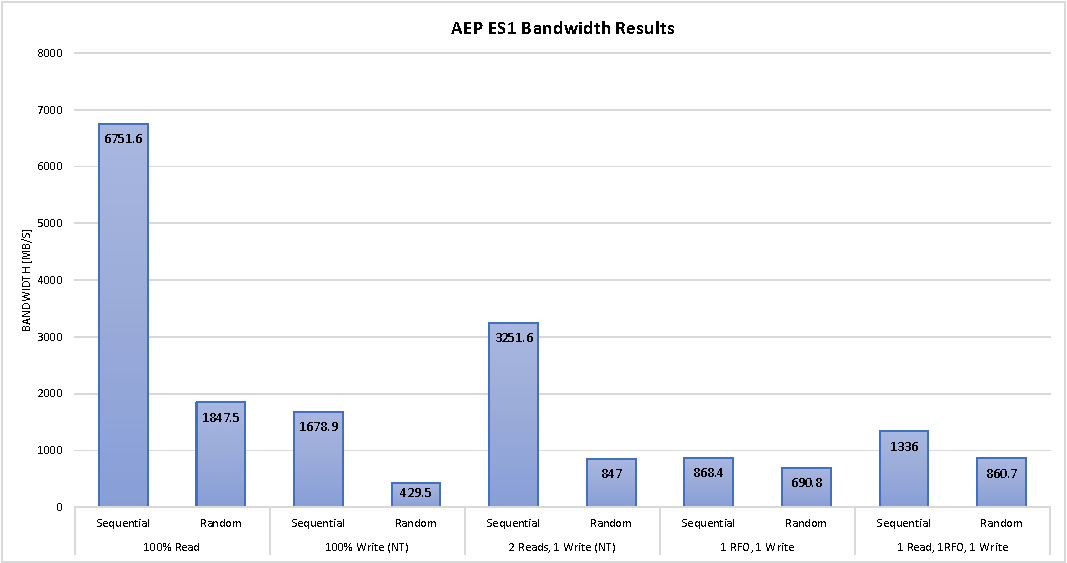
\includegraphics[scale=0.5]{charts/aep_eval_bandwidth-crop.pdf}
\end{figure}

\begin{figure}
    \centering
    \caption{Idle Latency Evaluation of Test System against Intel Reference}\label{chart:aep:idle}
    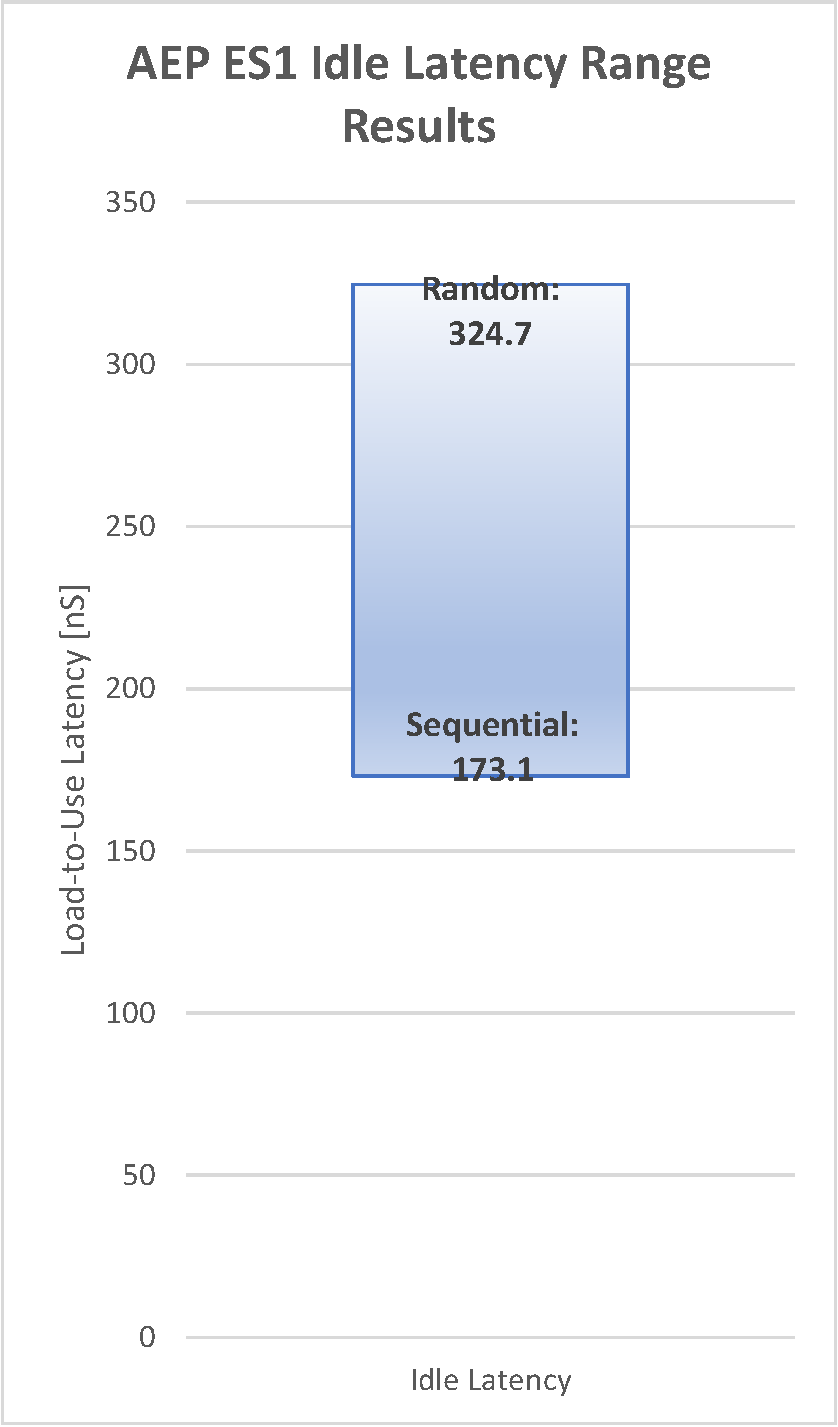
\includegraphics[scale=0.5]{charts/aep_eval_idle_latency-crop.pdf}
\end{figure}

\begin{figure}
    \centering
    \caption{Random Read Load Latency Evaluation of Test System against Intel Reference}\label{chart:aep:read}
    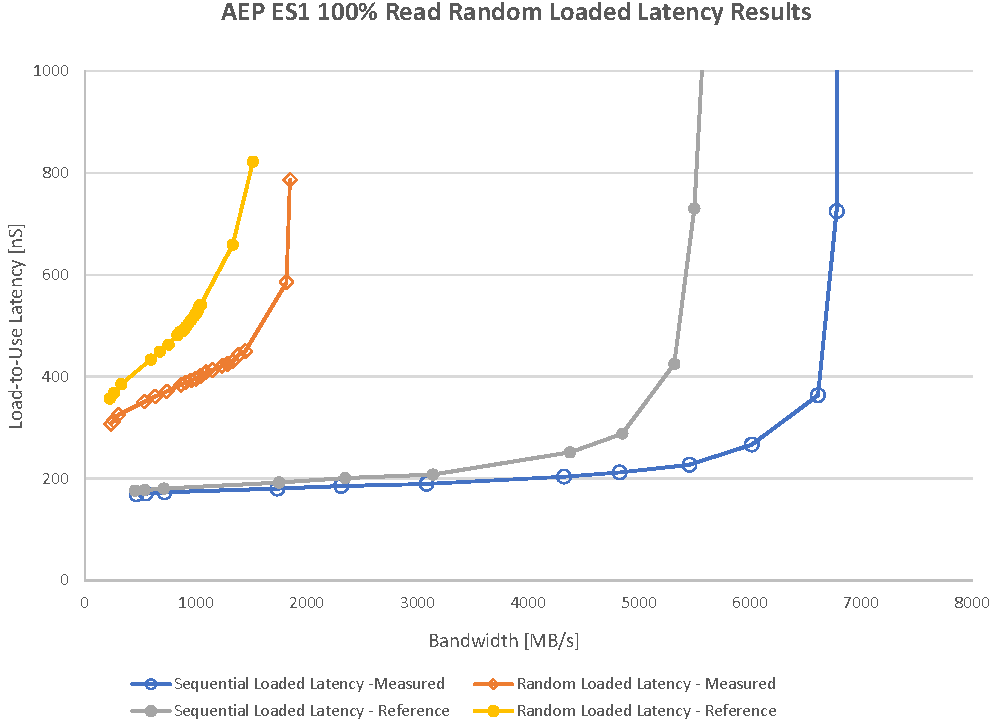
\includegraphics[scale=0.5]{charts/aep_eval_random_read_load_latency-crop.pdf}
\end{figure}

\begin{table}
    \centering
    \caption{Test System versus Intel Reference}\label{mlc:reference}
    \begin{tabular}{@{}cl@{}}
        Test Description & Figure \\ \toprule
        Idle Memory Latency & \ref{chart:aep:idle} \\
        Loaded Memory Bandwidth & \ref{chart:aep:bw} \\
        Random Read Latency & \ref{chart:aep:read} \\ \bottomrule
    \end{tabular}%
\end{table}


Because the early results I was observing were surprising, I spent time to verify that I was
using the tools properly by reproducing the original Intel results.  This exercise was
useful because it allowed me to identify undocumented options being used by Intel in
their own evaluation, understanding how to enable their ``persistent memory'' mode in
the tests, and validate that I was able to obtain comparable results, suggesting that
I was indeed testing the hardware appropriately.  Ultimately, I did adjust my own data
collection techniques to ensure that I was enabling persistent memory mode.

Intel provided benchmark numbers for three tests and the scripts to repeat their tests
on the actual test system. These tests, and the results, are shown in Table \ref{mlc:reference}.
The results were slightly faster, as I was using a newer system, but within 20\% of the original
Intel reference numbers.

Figure \ref{chart:aep:bw} shows the bandwidth evaluation; the test system has somewhat better bandwidth than the Intel reference system.

Figure \ref{chart:aep:idle} shows the idle latency evaluation; the test system has somewhat better idle latency than the Intel reference system.

Figure \ref{chart:aep:read} shows the random read evaluation for the
test system.  Again, it is somewhat better than the Intel reference
system results.

These better measurements are indicative of the fact that the system
under test was more recent hardware than the original Intel reference
system.  The improvements are modest (approximately 10\%) and seem
to be consistent across the various tests.  Thus, I concluded that my
experimental setup was correct.

Evaluating how Intel was performing these tests provided me with
insight into how Intel was using the \acs{MLC} test program.  Notably
they were using undocumented switches and generated specific
configurations for testing that indicated specific optimization for
their target benchmarks.  For example, Intel allocates \textbf{two}
cores (``threads'') per NVM DIMM module for performing their load
generation.  As a result, in my own testing I used a varied number of
threads to evaluate this area further.

\subsection{Non-Temporal Baseline Measurements}

This section describes the information for \textbf{non-temporal move}
operations on the same node. Because these are done as non-temporal
move operations, they bypass the cache and write directly to the actual
memory.  Note that I discuss the failure domain in greater detail in 
\S \ref{section:model:failure}.
The transfer involved here is sufficiently large that the impact of 
the memory controller caching does not impact behavior.


\subsubsection{DRAM}\label{baseline:dram}

\begin{figure}
    \centering
    \caption{Baseline Measurement of DRAM Non-Temporal Write on the same NUMA Node}\label{chart:baseline:dram}
    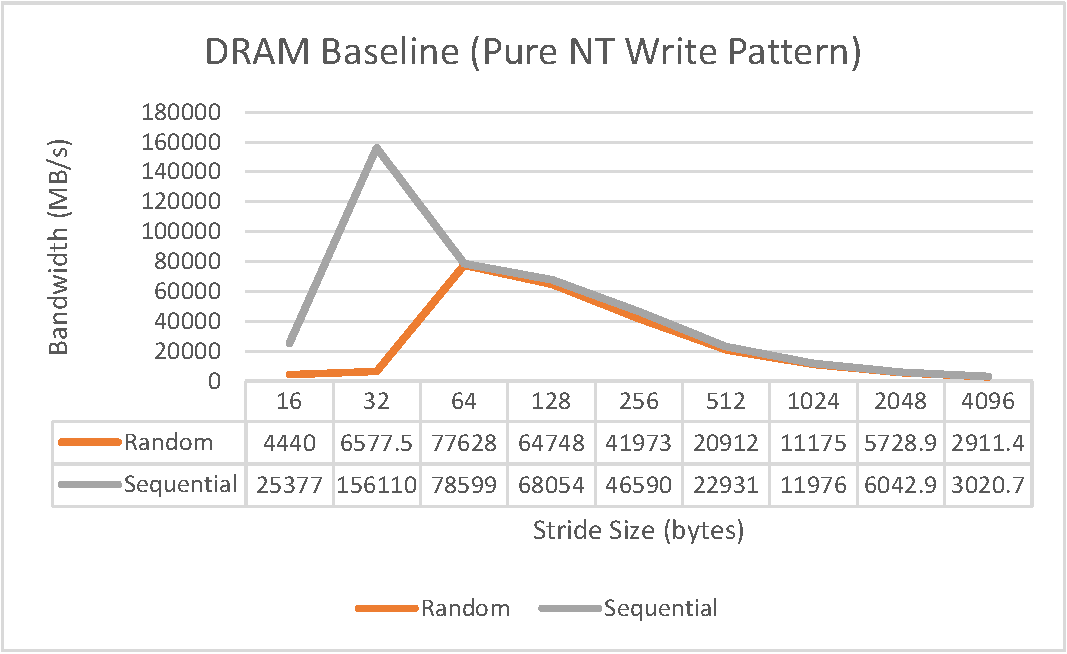
\includegraphics[width=1\textwidth]{charts/dram-baseline-nt-write-same-node-crop.pdf}
\end{figure}

Baseline testing was done using the switches:

\begin{verbatim}
    --loaded_latency -d0 -t10 -W6 -l1024 -T 
        -odata/bw_ctl_pmem0p1_seq_W6-0_23_400000_dram.dat
\end{verbatim}

The file \verb+data/bw_ctl_pmem0p1_seq_W6-0_23_400000_dram.dat+ contained the confirmation information
for the specific test layout:

\begin{verbatim}
0       W6 seq 400000 dram 0
1-23    W6 seq 400000 dram 0
\end{verbatim}

This drives the test to use core 0 for latency measurements, and cores 1-23 for load generation.

Note that the \verb+-l+ option was varied depending upon the ``stride'' size (unit of data handling).
The control file specified the disposition of the individual CPUs

I do not report results for any other DRAM tests.

Figure \ref{chart:baseline:dram} shows a baseline test for
non-temporal read operations with various stride sizes.  This
establishes the ``optimal'' performance using dynamic memory. One core
is used to measure the loaded bandwidth, the other 23 cores are used
to generate load.  It is interesting to note that a 32 byte stride
size provides the best bandwidth measurement (1600000 MB/s 
sequential).  I suspect this is due to prefetching and caching 
behavior, though I
did not validate this theory.  The 64 byte stride size (one cache line)
provides half this (80000 MB/s). 

\subsubsection{NVM}\label{baseline:nvm}

\begin{figure}[b]
\centering
    \caption{Baseline Measurement of NVM Non-Temporal Write on the same NUMA Node}\label{chart:baseline:nvm}
    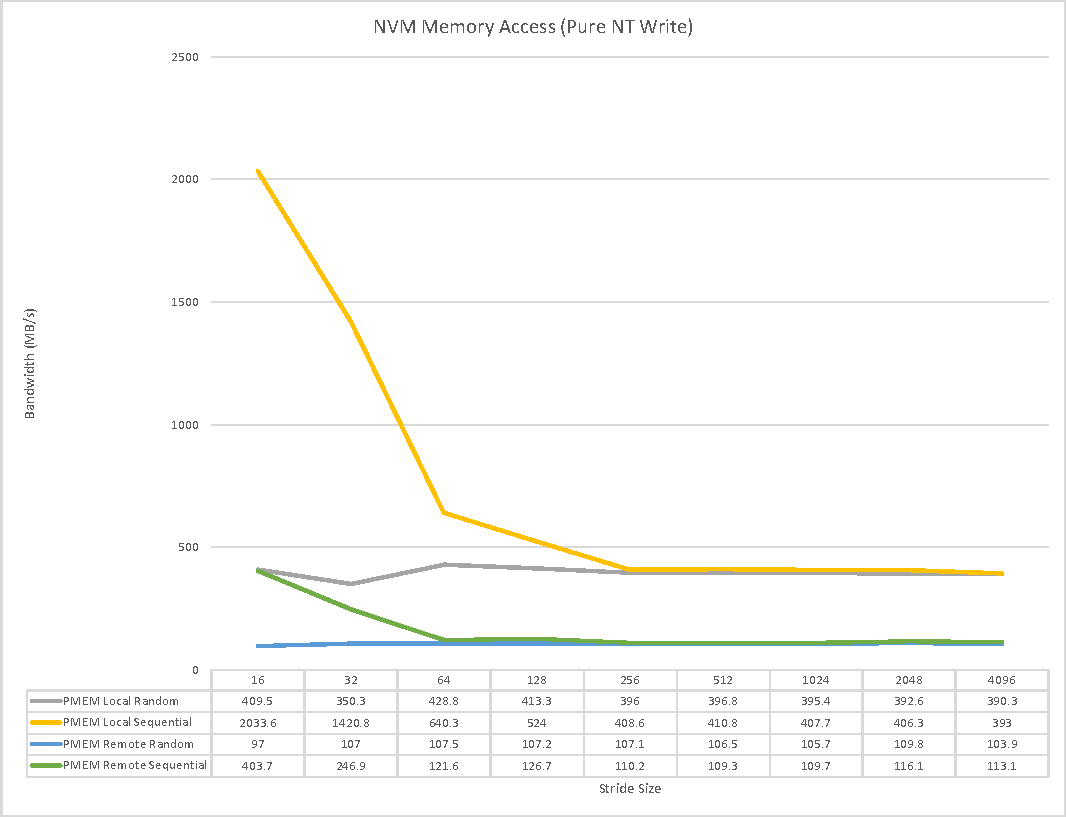
\includegraphics[width=1\textwidth]{charts/nt-write-both-nodes-crop.pdf}
\end{figure}

Baseline testing was done using the switches:

\begin{verbatim}
    --loaded_latency -d0 -t10 -W6 -l64 \
      -odata/bw_ctl_pmem0p1_seq_W6-0_23_400000_pmem.dat}
\end{verbatim}

The file \verb+data/bw_ctl_pmem0p1_seq_W6-0_23_400000_dram.dat+ contained the confirmation information
for the specific test layout:

\begin{verbatim}
0    W6 seq 400000 pmem /mnt/pmem0p1
1-23 W6 seq 400000 pmem /mnt/pmem0p1
\end{verbatim}

The \verb+pmem+ directive is used to put the test utility into ``persistent memory'' testing mode.
The final value is the name of the directory to use.  It \textbf{must} be a persistent memory
to run this test.  Otherwise the test will refuse to run.

Figure \ref{chart:baseline:nvm} shows a baseline test for non-temporal
read operations.  In this case the measurements show both NUMA local
as well as cross-NUMA node persistent memory values.  Note that
these values are substantialy below the DRAM values by more than an
order of magnitude.  The cross-node performance was surprising to
me, as I would have expected the memory bandwidth to be the rate
limiting issue, but apparently there is some consideration in the NUMA
memory management that imposes a substantial performance restriction.

Equally surprising is that the cost of random versus sequential
operations converge fairly quickly

\subsection{Read}\label{mlc:r}

I tested specific configurations for random read and those are
reported in this section in more detail than likely anyone will read.
Note that these are cached reads.

\subsubsection{Random}\label{mlc:r:rand}
\begin{figure}
    \centering
    \caption{Random Read (R)}\label{chart:random:read}
    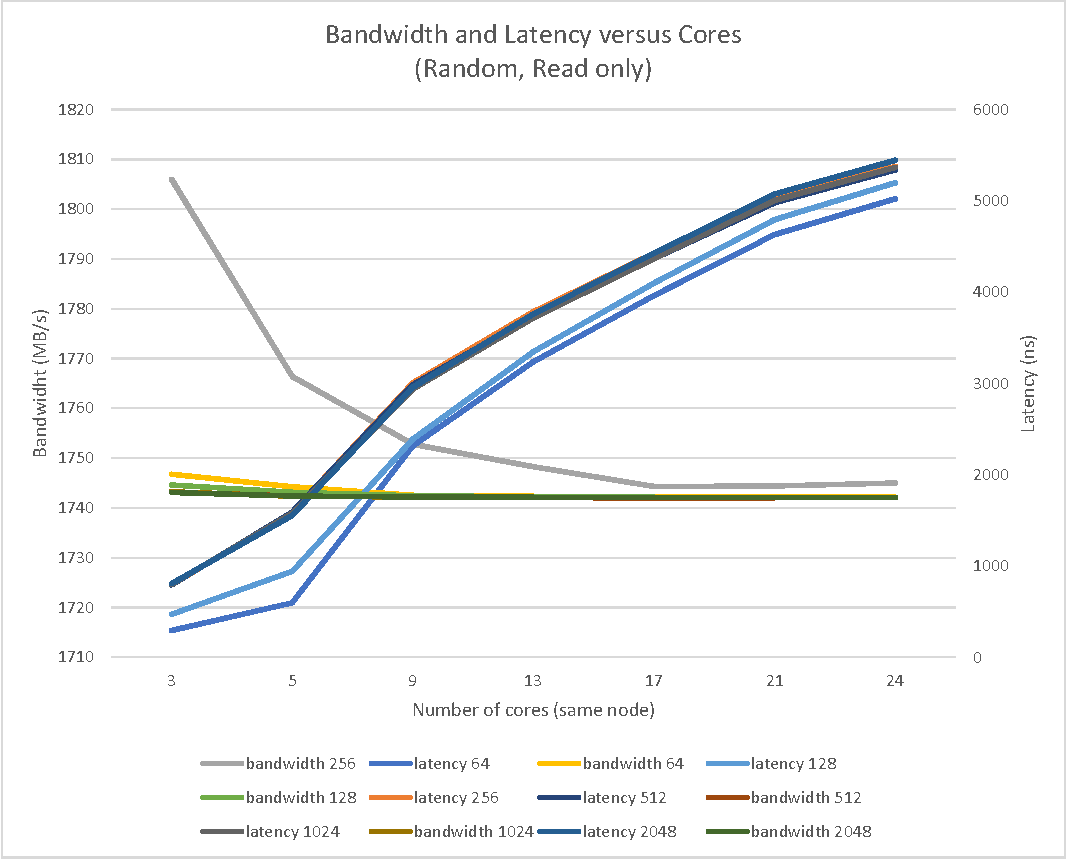
\includegraphics[scale=0.5]{charts/random-r-crop.pdf}
\end{figure}

Random read testing was done using the switches:

\begin{verbatim}
    --loaded_latency -d0 -t10 -R -l64 \
     -odata/bw_ctl_pmem0p1_rand_R-0_12_400000_pmem.dat
\end{verbatim}

Note that the \verb+-l+ parameter was varied for different
stride sizes, and the configuration file was varied to control
the number of cores being used in the test.

The file \verb+data/bw_ctl_pmem0p1_rand_R-0_23_400000_dram.dat+ contained the confirmation information
for the specific test layout:

\begin{verbatim}
0	R rand 400000 pmem /mnt/pmem0p1
1-12	R rand 400000 pmem /mnt/pmem0p1
\end{verbatim}

The results from this test are shown in Figure \ref{chart:random:read}.
Note that the chart shows both bandwidth and latency in a single
chart; bandwidth is along the left y-axis and latency is along the
right x-axis.

Random read performance shows quite well at two cores, which suggests
that may be why Intel performance figures have been computed using two
cores for loading with 256 byte stride sizes.

These figures help better observe the nature of concurrency costs when
accessing non-volatile memory.

\subsubsection{Sequential}\label{mlc:r:seq}

\begin{figure}
    \centering
    \caption{Sequential Read (R)}\label{chart:sequential:read}
    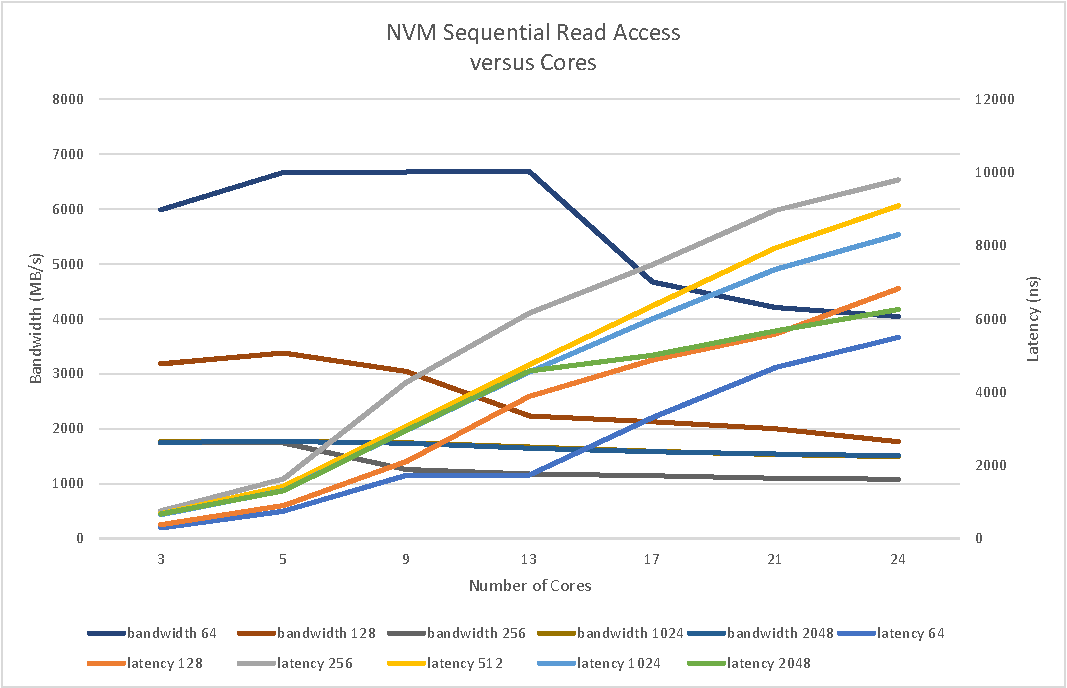
\includegraphics[scale=0.5]{charts/sequential-r-crop.pdf}
\end{figure}

Sequential read is a common operation; it is also one that I would
expect is an optimal case, benefitting from caches and prefetch
logic.

Sequential read testing was done using the switches:

\begin{verbatim}
    --loaded_latency -d0 -t10 -R -l64 \
    -odata/bw_ctl_pmem0p1_seq_R-0_20_400000_pmem.dat
\end{verbatim}

Note that the \verb+-l+ parameter was varied for different
stride sizes, and the configuration file was varied to control
the number of cores being used in the test.

The file \verb+data/bw_ctl_pmem0p1_seq_R-0_20_400000_pmem.dat+ contained the confirmation information
for the specific test layout:

\begin{verbatim}
0	R seq 400000 pmem /mnt/pmem0p1
1-20	R seq 400000 pmem /mnt/pmem0p1
\end{verbatim}

Figure \ref{chart:sequential:read} shows the results from this test.
The performance for sequential read is substantially better than
random read (see \S \ref{mlc:r:rand}), both in terms of bandwidth
and latency.

\subsection{Mixed Read/Write 2:1}

This workload consists of a mixed read/write at two-to-one ratio and
is considered for both random and sequential access patterns.

\subsubsection{Random}

\begin{figure}
    \centering
    \caption{Random 2:1 Read/Write (W2)}\label{chart:random:W2}
    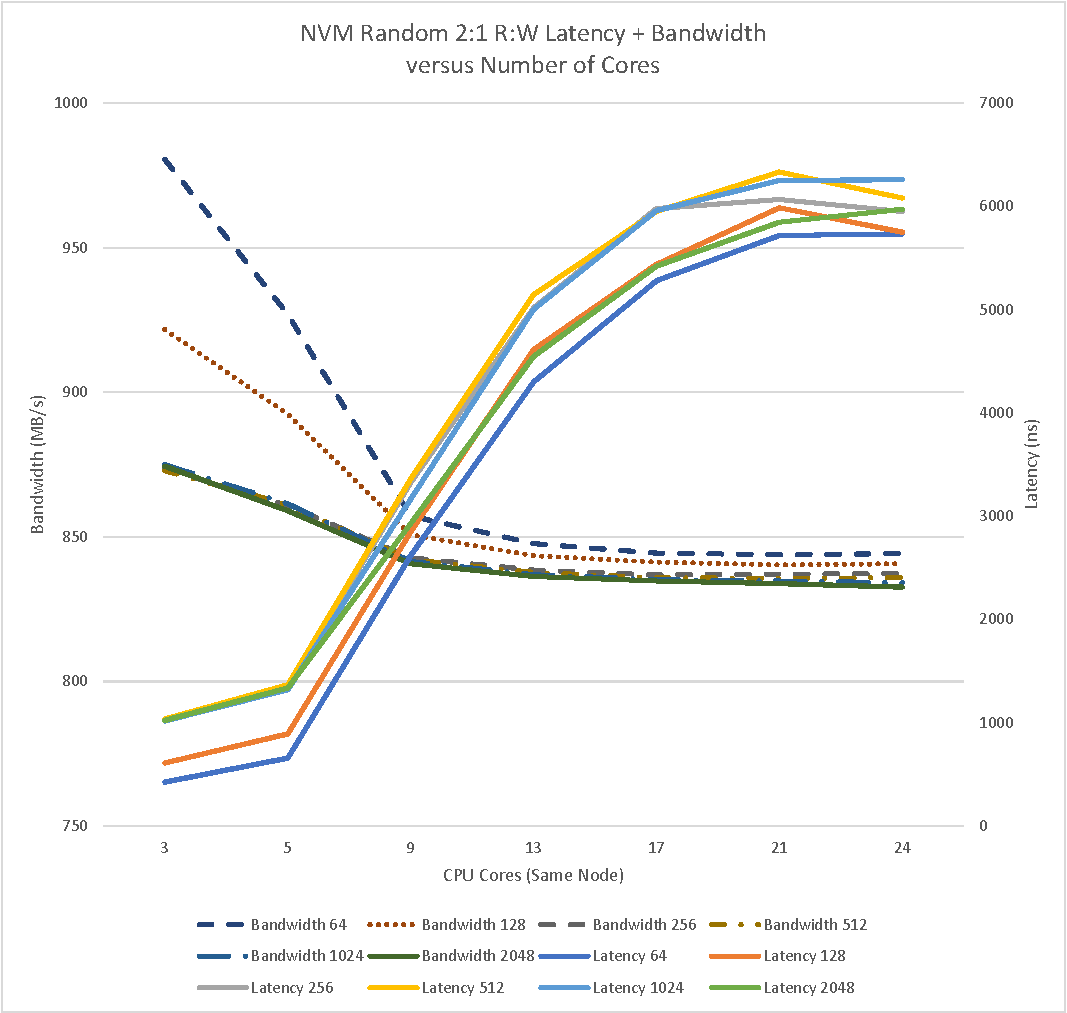
\includegraphics[scale=0.5]{charts/random-w2-crop.pdf}
\end{figure}

Random read testing was done using the switches:

\begin{verbatim}
    --loaded_latency -d0 -t10 -W2 -l64 \
    -odata/bw_ctl_pmem0p1_rand_W2-0_20_400000_pmem.dat
\end{verbatim}

Note that the \verb+-l+ parameter was varied for different
stride sizes, and the configuration file was varied to control
the number of cores being used in the test.

The file \verb+data/bw_ctl_pmem0p1_rand_W2-0_20_400000_pmem.dat+ contained the confirmation information
for the specific test layout:

\begin{verbatim}
0	W2 rand 400000 pmem /mnt/pmem0p1
1-20	W2 rand 400000 pmem /mnt/pmem0p1
\end{verbatim}

Figure \ref{chart:random:W2} shows the results from this test.

The results here suggest that bandwidth decreases with more cores,
possibly due to some contention issues, but appears to be stable
after 12 or so cores are active, though latency rises rapidly
above four cores.

\subsubsection{Sequential}

\begin{figure}
    \centering
    \caption{Sequential 2:1 Read/Write (W2)}\label{chart:sequential:W2}
    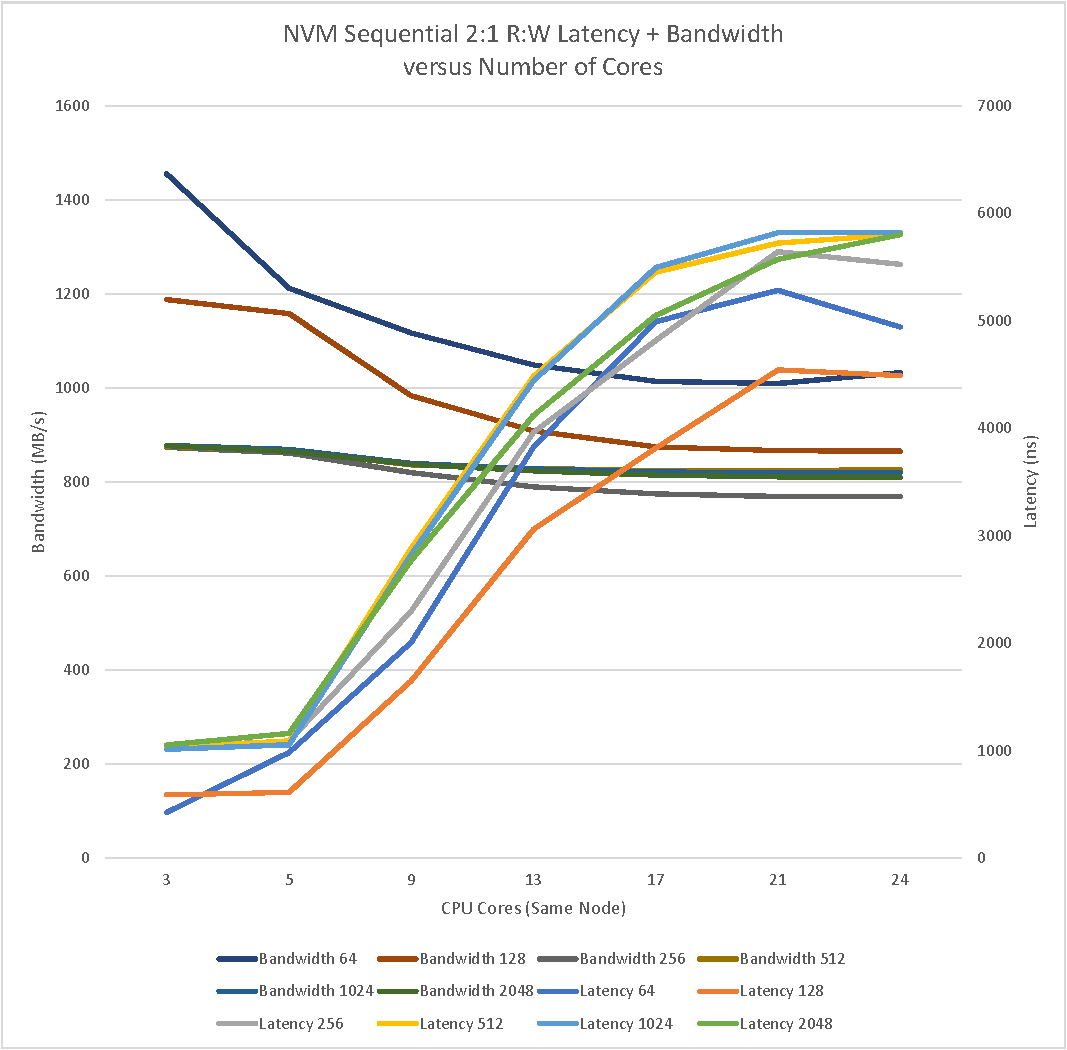
\includegraphics[scale=0.5]{charts/sequential-w2-crop.pdf}
\end{figure}

Sequential read testing was done using the switches:

\begin{verbatim}
    --loaded_latency -d0 -t10 -W2 -l64 \
    -odata/bw_ctl_pmem0p1_seq_W2-0_20_400000_pmem.dat
\end{verbatim}

Note that the \verb+-l+ parameter was varied for different
stride sizes, and the configuration file was varied to control
the number of cores being used in the test.

The file \verb+data/bw_ctl_pmem0p1_seq_W2-0_20_400000_pmem.dat+ contained the confirmation information
for the specific test layout:

\begin{verbatim}
0	W2 seq 400000 pmem /mnt/pmem0p1
1-20	W2 seq 400000 pmem /mnt/pmem0p1
\end{verbatim}

Figure \ref{chart:sequential:W2} shows the results from this test.

Bandwidth results are more consistent for this workload.

\subsection{Mixed Sequential Read/Write 3:1}

\begin{figure}
    {\centering
    \caption{Sequential 3:1 Read/Write (W3)}\label{chart:sequential:w3}
    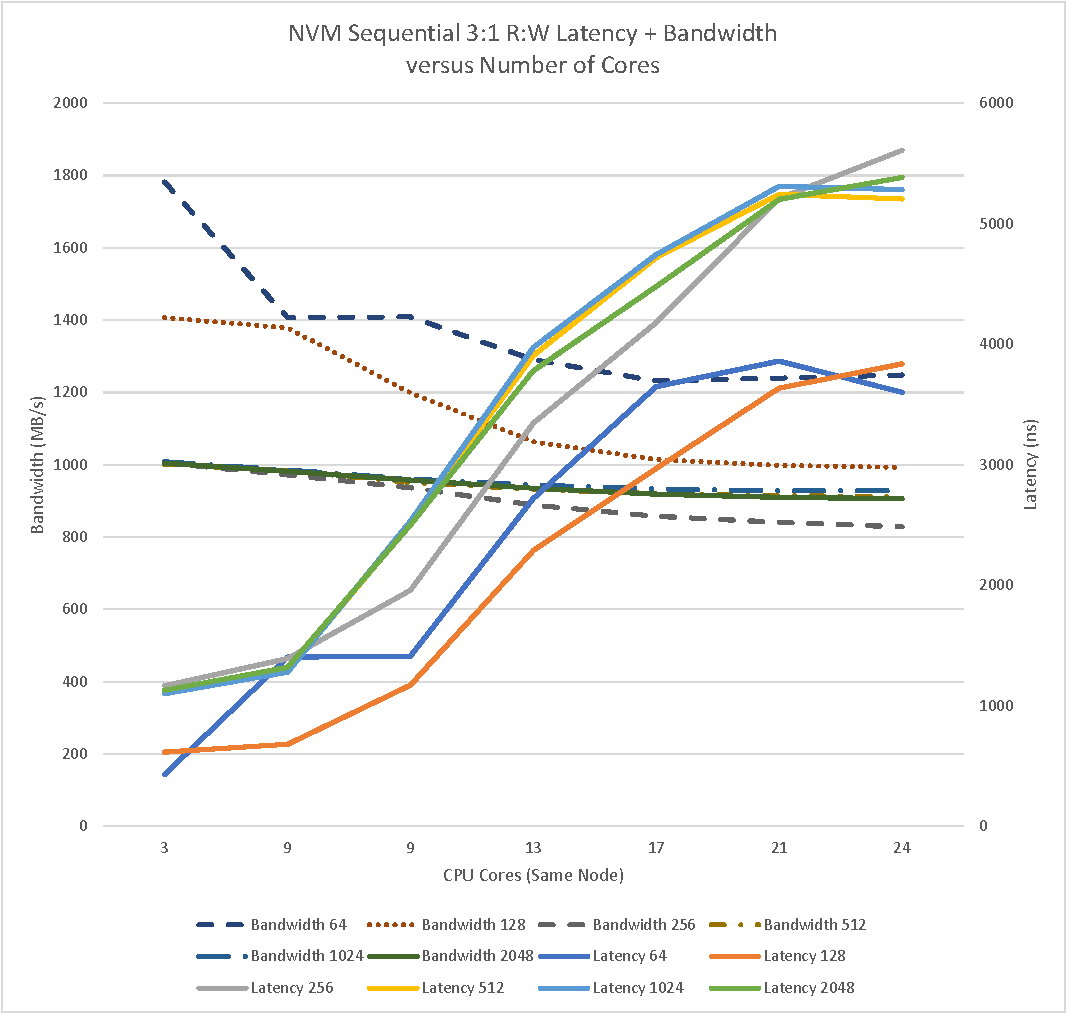
\includegraphics[scale=0.5]{charts/sequential-w3-crop.pdf}
    }
\end{figure}

Sequential read/write testing using a three-to-one read-to-write ratio was 
done using the switches:

\begin{verbatim}
    --loaded_latency -d0 -t10 -W3 -l64 \
    -odata/bw_ctl_pmem0p1_seq_W3-0_20_400000_pmem.dat
\end{verbatim}

Note that the \verb+-l+ parameter was varied for different
stride sizes, and the configuration file was varied to control
the number of cores being used in the test.

The file \verb+data/bw_ctl_pmem0p1_seq_W3-0_20_400000_pmem.dat+ contained the confirmation information
for the specific test layout:

\begin{verbatim}
0	W3 seq 400000 pmem /mnt/pmem0p1
1-20	W3 seq 400000 pmem /mnt/pmem0p1
\end{verbatim}

Figure \ref{chart:sequential:w3} shows the results from this test.

These results show a much larger lack of divergence than seen with
prior workloads.  Cache line impact seems to be fairly
substantial with the 64 byte stride size showing markedly better
performance than other stride sizes, while 128 and 256 byte stride
sizes showing better latency than other stride values. 

\subsection{Mixed Read/Write 1:1}

In this test, a one-to-one read-to-write workload is used with
a random read/write access pattern; caching is eanbled.
Results are provided for both random and sequential access
patterns.

\subsubsection{Random}

\begin{figure}
    \centering
    \caption{Random 1:1 Read/Write (W5)}\label{chart:random:W5}
    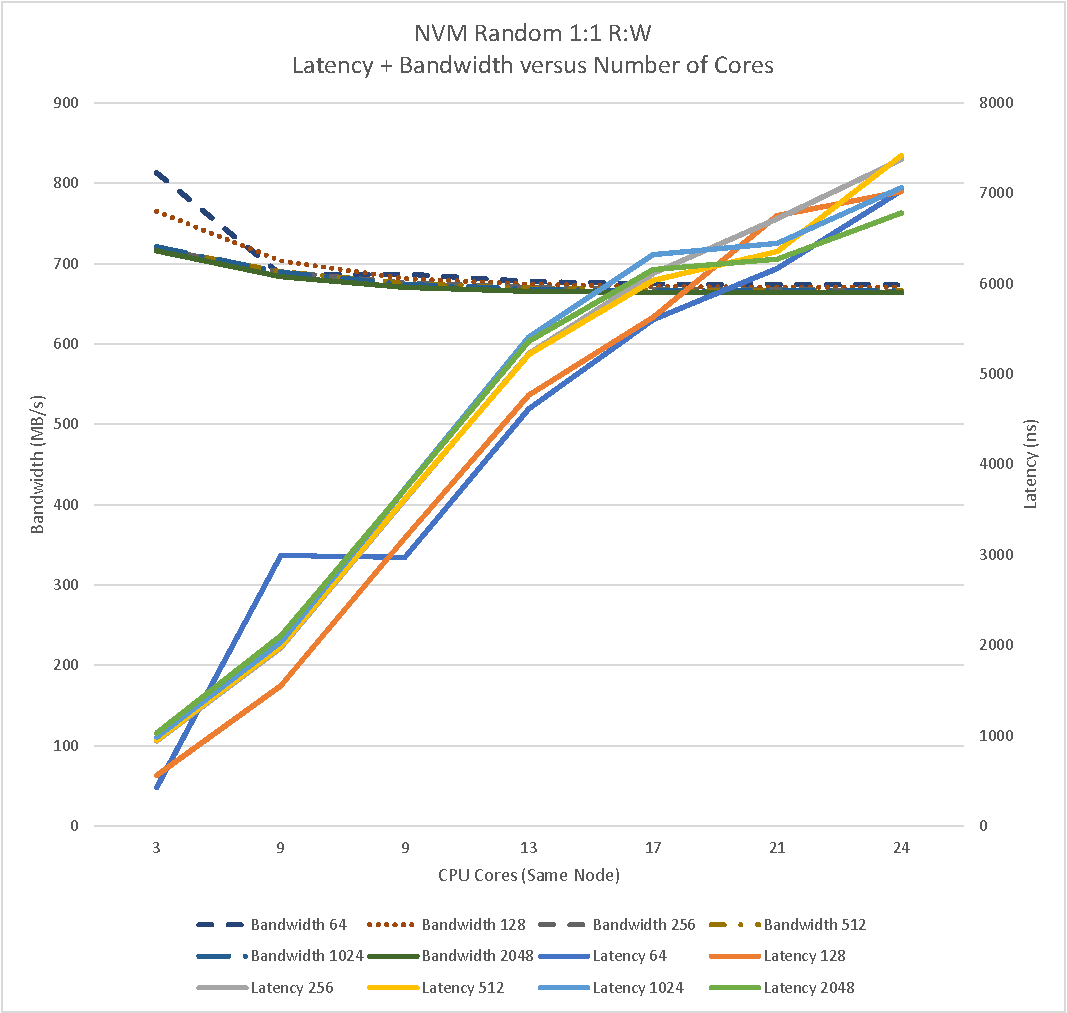
\includegraphics[scale=0.5]{charts/random-w5-crop.pdf}
\end{figure}

The following switches were used:

\begin{verbatim}
    --loaded_latency -d0 -t10 -W5 -l64 \
    -odata/bw_ctl_pmem0p1_rand_W5-0_20_400000_pmem.dat
\end{verbatim}

Note that the \verb+-l+ parameter was varied for different
stride sizes, and the configuration file was varied to control
the number of cores being used in the test.

The file \verb+data/bw_ctl_pmem0p1_rand_W5-0_20_400000_pmem.dat+ contained the confirmation information
for the specific test layout:

\begin{verbatim}
0	W5 rand 400000 pmem /mnt/pmem0p1
1-20	W5 rand 400000 pmem /mnt/pmem0p1
\end{verbatim}

Figure \ref{chart:random:W5} shows the results from this test.

Interestingly, performance here is remarkably uniform regardless
of stride size.

\subsubsection{Sequential}

\begin{figure}
    \centering
    \caption{Sequential 1:1 Read to Write (W5)}\label{chart:sequential:W5}
    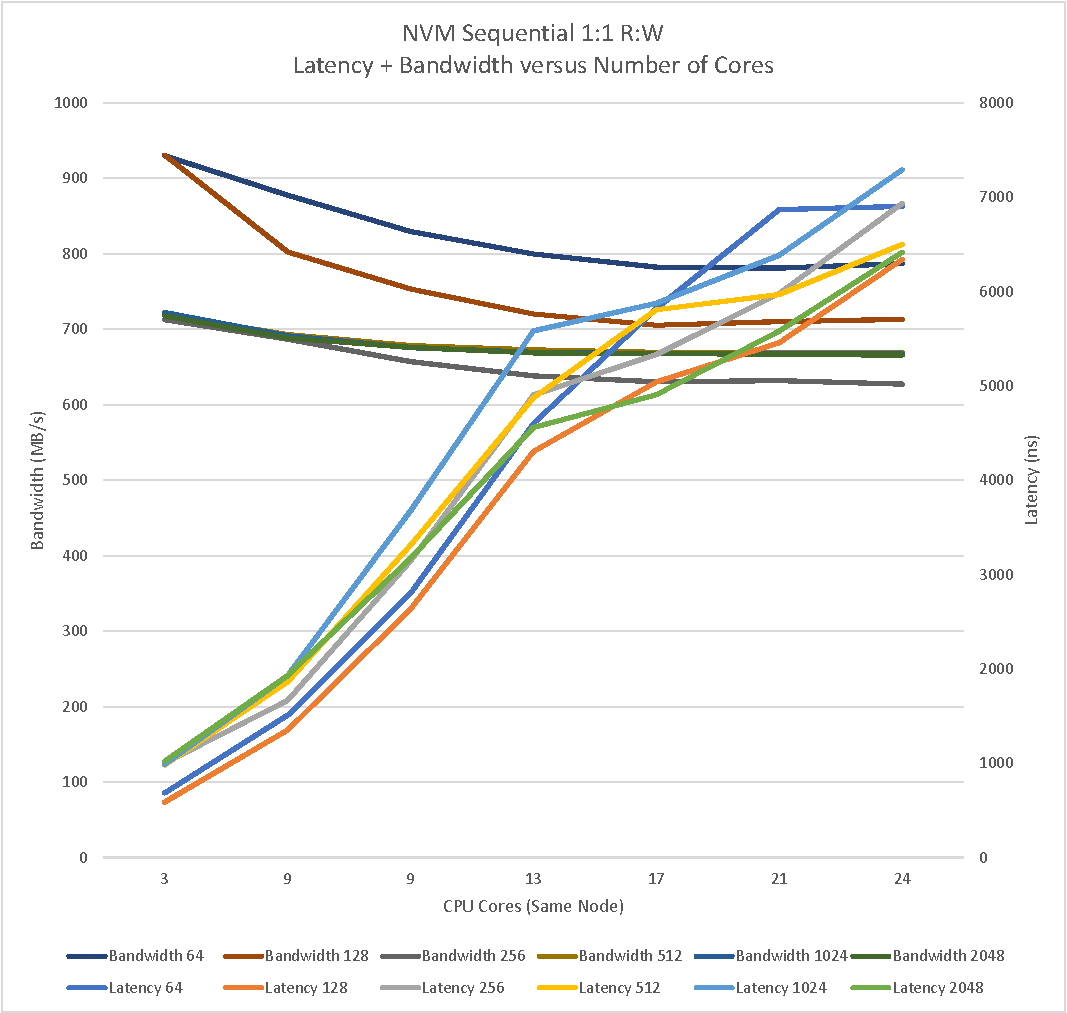
\includegraphics[scale=0.5]{charts/sequential-w5-crop.pdf}
\end{figure}


The testing was done using the switches:

\begin{verbatim}
    --loaded_latency -d0 -t10 -W5 -l64 \
    -odata/bw_ctl_pmem0p1_seq_W5-0_20_400000_pmem.dat
\end{verbatim}

Note that the \verb+-l+ parameter was varied for different
stride sizes, and the configuration file was varied to control
the number of cores being used in the test.

The file \verb+data/bw_ctl_pmem0p1_seq_W5-0_20_400000_pmem.dat+ contained the confirmation information
for the specific test layout:

\begin{verbatim}
0	W5 seq 400000 pmem /mnt/pmem0p1
1-20	W5 seq 400000 pmem /mnt/pmem0p1
\end{verbatim}

Figure \ref{chart:sequential:W5} shows the results from this test.


\subsection{Non-Temporal Write}

The non-temporal tests explictly avoid the processor cache;
as such they provide a better measure of pure performance for
the underlying non-volatile memory.  The tests in this case
work for both random and sequential access patterns.

The workload used for these tests is a pure \textbf{write}
workload.  This is useful when considering predominately write
usage patterns, such as for logs.

\subsubsection{Random}

\begin{figure}
    \centering
    \caption{Random Non-Temporal Write (W6)}\label{chart:random:W6}
    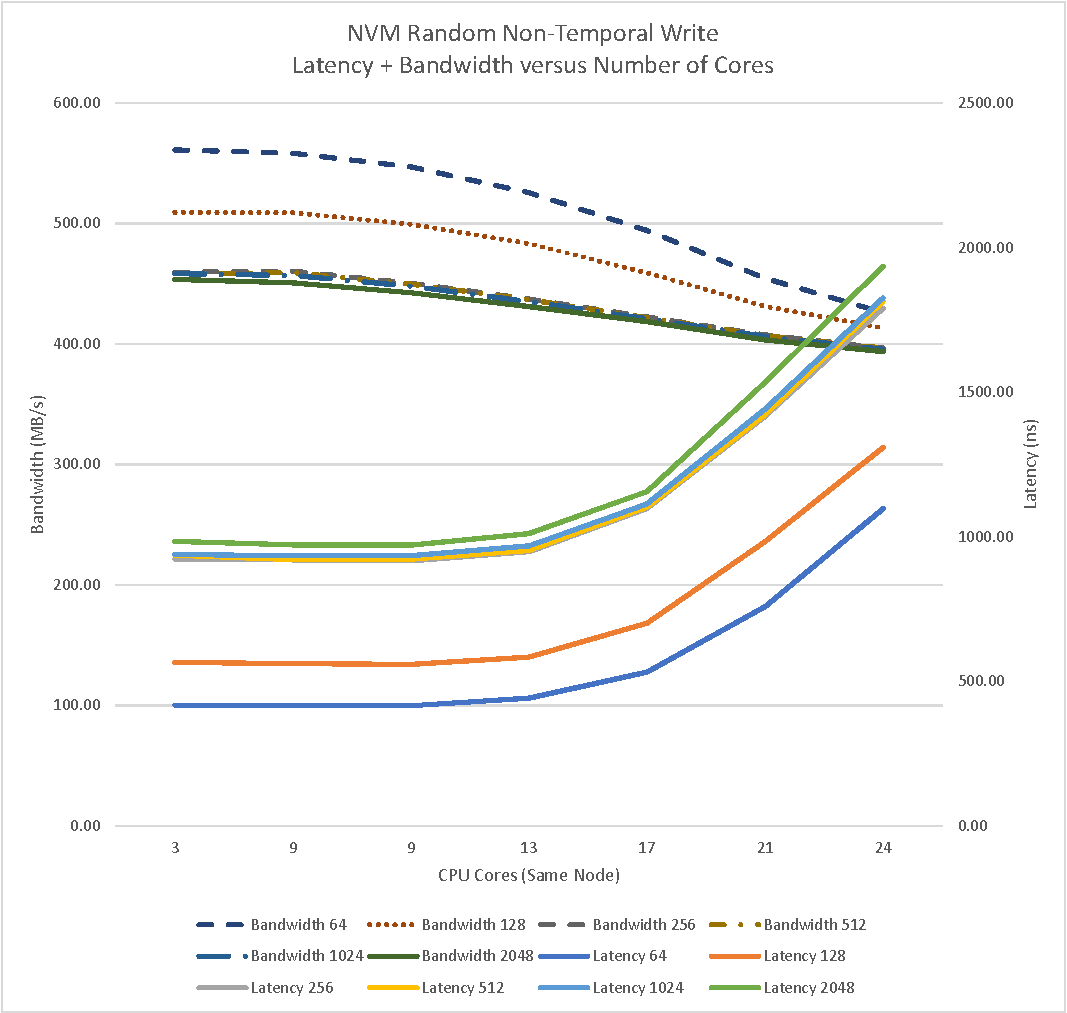
\includegraphics[scale=0.5]{charts/random-w6-crop.pdf}
\end{figure}

In this test, a one-to-one read-to-write workload is used with
a random read/write access pattern; caching is eanbled.  The
following switches were used:

\begin{verbatim}
    --loaded_latency -d0 -t10 -W6 -l64 \
    -odata/bw_ctl_pmem0p1_rand_W6-0_20_400000_pmem.dat
\end{verbatim}

Note that the \verb+-l+ parameter was varied for different
stride sizes, and the configuration file was varied to control
the number of cores being used in the test.

The file \verb+data/bw_ctl_pmem0p1_rand_W6-0_20_400000_pmem.dat+ contained the confirmation information
for the specific test layout:

\begin{verbatim}
0	W6 rand 400000 pmem /mnt/pmem0p1
1-20	W6 rand 400000 pmem /mnt/pmem0p1
\end{verbatim}

Figure \ref{chart:random:W6} shows the results from this test.

Interestingly, performance here is remarkably uniform regardless
of stride size.  Performance generally seems best with 64 byte
strides, with corresponding lower latency as well.


\subsubsection{Sequential}

\begin{figure}
    \centering
    \caption{Sequential Non-Temporal Write (W6)}\label{chart:sequential:W6}
    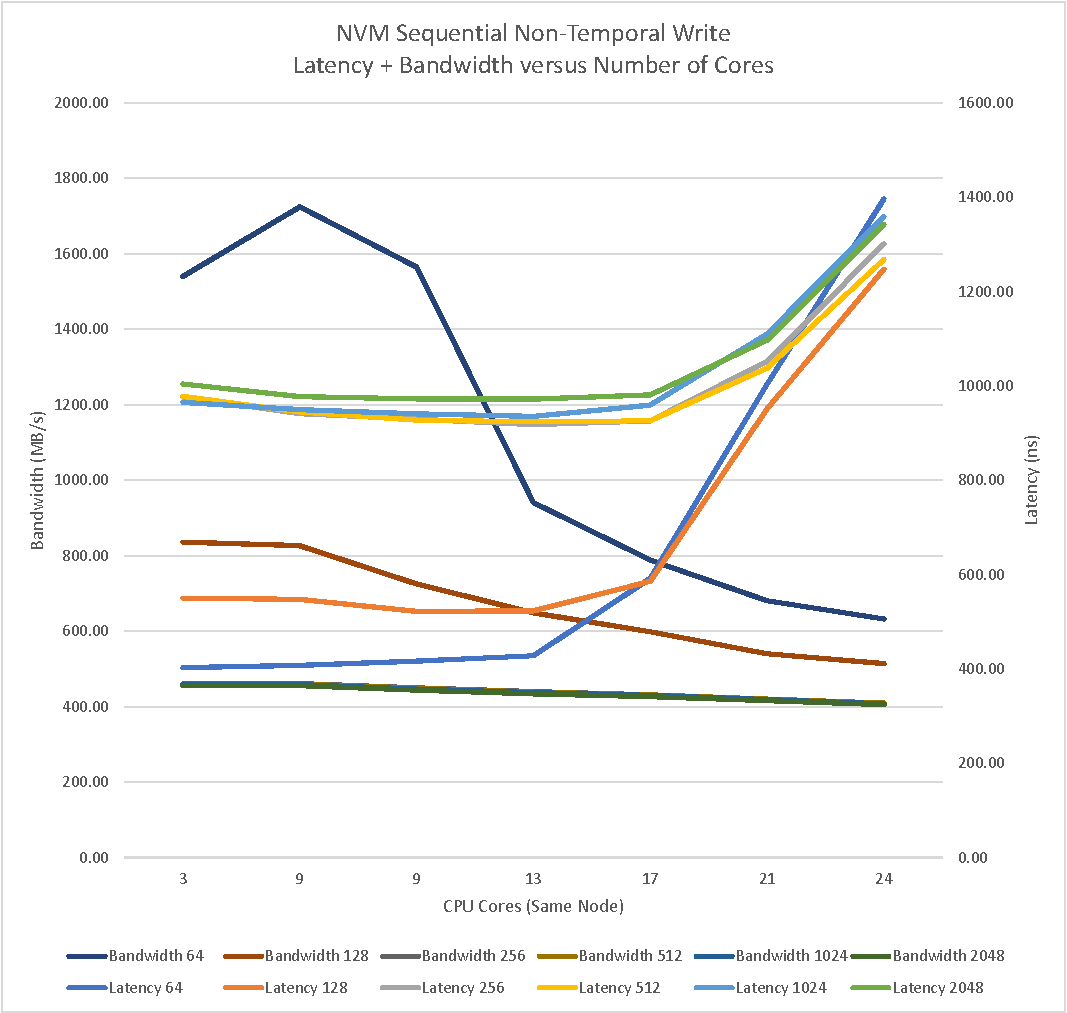
\includegraphics[scale=0.5]{charts/sequential-w6-crop.pdf}
\end{figure}

Sequential read/write testing using a three-to-one read-to-write ratio was 
done using the switches:

\begin{verbatim}
    --loaded_latency -d0 -t10 -W6 -l64 \
    -odata/bw_ctl_pmem0p1_seq_W6-0_20_400000_pmem.dat
\end{verbatim}

Note that the \verb+-l+ parameter was varied for different
stride sizes, and the configuration file was varied to control
the number of cores being used in the test.

The file \verb+data/bw_ctl_pmem0p1_seq_W6-0_20_400000_pmem.dat+ contained the confirmation information
for the specific test layout:

\begin{verbatim}
0	W6 seq 400000 pmem /mnt/pmem0p1
1-20	W6 seq 400000 pmem /mnt/pmem0p1
\end{verbatim}

Figure \ref{chart:sequential:W6} shows the results from this test.

The results here do quite well with 64 byte strides both in
terms of latency and bandwidth.  The performance drops with
increased processor contention above 8 cores, with latency
increasing substantially above 12 cores.

\subsection{Non-Temporal Read/Write 2:1}

This workload is in fact a \textbf{cached} read with 
\textbf{non-cached} workload mix.  Writes are done using
non-temporal instructions, while reads are done using CPU
caching.

It uses a two-to-one read-to-write workload pattern. Non-temporal
writes will perform cache invalidation, so a subsequent read of
the memory region would force a reload from memory.

\subsubsection{Random}

\begin{figure}
    \centering
    \caption{Random 2:1 Read to Non-Temporal Write (W7)}\label{chart:random:W7}
    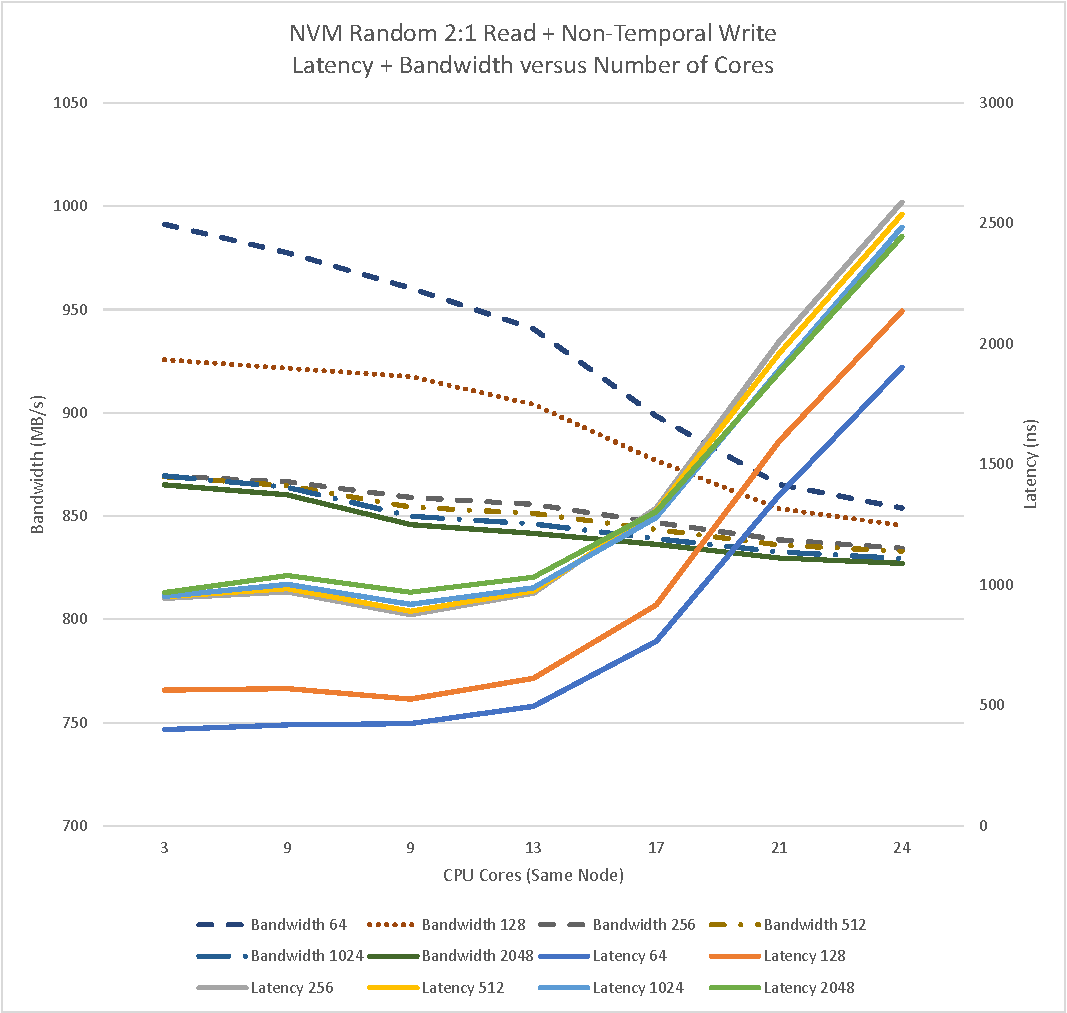
\includegraphics[scale=0.5]{charts/random-w7-crop.pdf}
\end{figure}

The following switches were used:

\begin{verbatim}
    --loaded_latency -d0 -t10 -W7 -l64 \
    -odata/bw_ctl_pmem0p1_rand_W7-0_20_400000_pmem.dat
\end{verbatim}

Note that the \verb+-l+ parameter was varied for different
stride sizes, and the configuration file was varied to control
the number of cores being used in the test.

The file \verb+data/bw_ctl_pmem0p1_rand_W7-0_20_400000_pmem.dat+ contained the confirmation information
for the specific test layout:

\begin{verbatim}
0	W7 rand 400000 pmem /mnt/pmem0p1
1-20	W7 rand 400000 pmem /mnt/pmem0p1
\end{verbatim}

Figure \ref{chart:random:W7} shows the results from this test.

The best bandwidth here is using 64 byte strides, with the
lowest latency for any stride size.  Bandwidth declines
and latency increases with increased core contention.

\subsubsection{Sequential}

\begin{figure}
    \centering
    \caption{Sequential 2:1 Read to Non-Temporal Write (W7)}\label{chart:sequential:W7}
    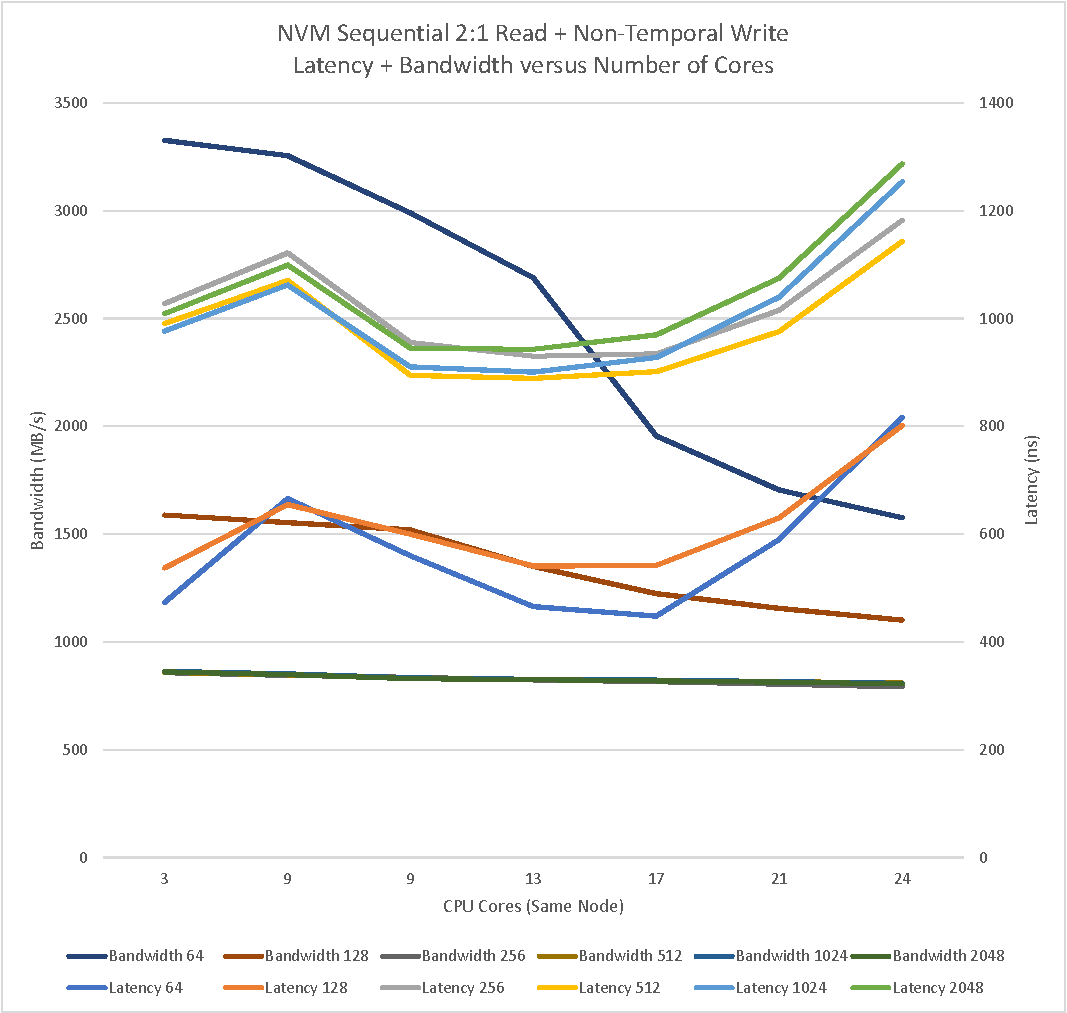
\includegraphics[scale=0.5]{charts/sequential-w7-crop.pdf}
\end{figure}

The testing was done using the switches:

\begin{verbatim}
    --loaded_latency -d0 -t10 -W7 -l64 \
    -odata/bw_ctl_pmem0p1_seq_W7-0_20_400000_pmem.dat
\end{verbatim}

Note that the \verb+-l+ parameter was varied for different
stride sizes, and the configuration file was varied to control
the number of cores being used in the test.

The file \verb+data/bw_ctl_pmem0p1_seq_W7-0_20_400000_pmem.dat+ contained the confirmation information
for the specific test layout:

\begin{verbatim}
0	W7 seq 400000 pmem /mnt/pmem0p1
1-20	W7 seq 400000 pmem /mnt/pmem0p1
\end{verbatim}

Figure \ref{chart:sequential:W7} shows the results from this test.

The best bandwidth is seen using a 64 byte stride; latency is
similar across the smaller stride sizes.  Bandwidth decreases
and latency increases with increased core contention for all
stride sizes, although there is a peculiar dip in latency when
half of the cores are active.

\subsection{Non-Temporal Read/Write 1:1}

This workload is a \textbf{cached} read with 
\textbf{non-cached} workload mix.  Writes are done using
non-temporal instructions, while reads are done using CPU
caching.

It uses a one-to-one read-to-write workload pattern. Non-temporal
writes will perform cache invalidation, so a subsequent read of
the memory region would force a reload from memory.

\subsubsection{Random}

\begin{figure}
    \centering
    \caption{Random 1:1 Read to Non-Temporal Write (W8)}\label{chart:random:W8}
    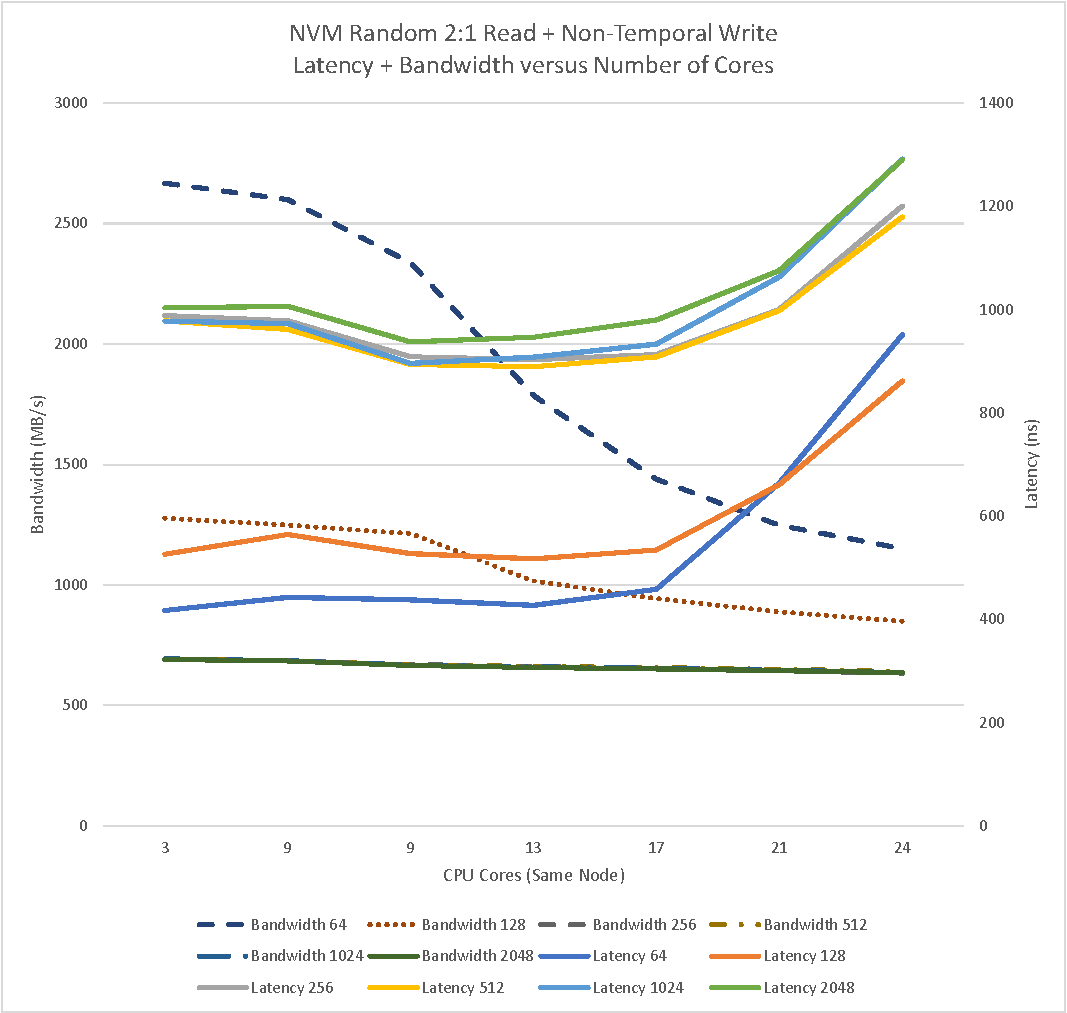
\includegraphics[scale=0.5]{charts/random-w8-crop.pdf}
\end{figure}

The following switches were used:

\begin{verbatim}
    --loaded_latency -d0 -t10 -W8 -l64 \
    -odata/bw_ctl_pmem0p1_rand_W8-0_20_400000_pmem.dat
\end{verbatim}

Note that the \verb+-l+ parameter was varied for different
stride sizes, and the configuration file was varied to control
the number of cores being used in the test.

The file \verb+data/bw_ctl_pmem0p1_rand_W8-0_20_400000_pmem.dat+ contained the confirmation information
for the specific test layout:

\begin{verbatim}
0	W8 rand 400000 pmem /mnt/pmem0p1
1-20	W8 rand 400000 pmem /mnt/pmem0p1
\end{verbatim}

Figure \ref{chart:random:W8} shows the results from this test.

The 64 byte stride shows the best bandwidth and lowest latency.
Bandwidth decreases and latency increases with increased core
contention.


\subsection{Sequential Streaming Triad Read/Non-Temporal Write 3:1}


\begin{figure}
    \centering
    \caption{Sequential 3:1 Read to Non-Temporal Write (streaming triad) (W10)}\label{chart:sequential:W10}
    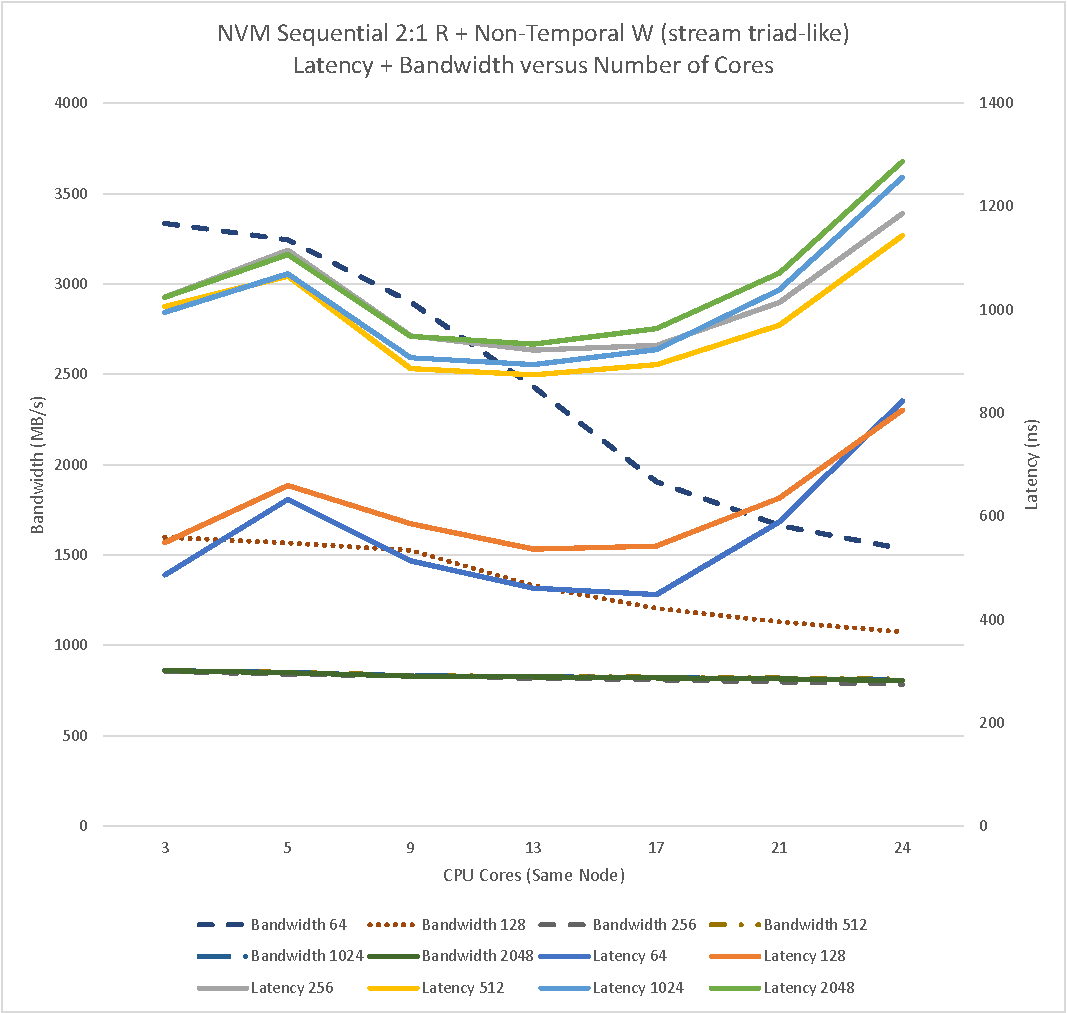
\includegraphics[scale=0.5]{charts/sequential-w10-crop.pdf}
\end{figure}

This workload is a streaming non-temporal write with
triad read operations.  There are three reads per write, with
the reads being triads (sequential reads).  This appears to
be a common high performance load for certain types of
video processing.

The testing was done using the switches:

\begin{verbatim}
    --loaded_latency -d0 -t10 -W10 -l64 \
    -odata/bw_ctl_pmem0p1_seq_W10-0_20_400000_pmem.dat
\end{verbatim}

Note that the \verb+-l+ parameter was varied for different
stride sizes, and the configuration file was varied to control
the number of cores being used in the test.

The file \verb+data/bw_ctl_pmem0p1_seq_W10-0_20_400000_pmem.dat+ contained the confirmation information
for the specific test layout:

\begin{verbatim}
0	W10 seq 400000 pmem /mnt/pmem0p1
1-20	W10 seq 400000 pmem /mnt/pmem0p1
\end{verbatim}

Figure \ref{chart:sequential:W10} shows the results from this test.

These results show best bandwidth for the 64 byte stride sizes.
Latency is lowest with minimal processor contention.  Other
stride sizes show substantially lower bandwidth results.

\section{Micro-Benchmark Results}\label{section:results:micro}

The micro-benchmark results are based upon custom tests that
I wrote as part of this investigation.  My focus in looking
at this performance was to better understand the interplay
between cache behavior and persistence operations.  By better
understanding the trade-offs involved, I can more easily reason
about constructing persistent data structures.

Throughout this section, I describe various flushing operation.
These are achieve by using specific instructions, including
the cache flush instructions: \texttt{clflush, clflushopt, clwb}
and the memory barrier instruction \texttt{sfence}, which
provides guarantees that all prior store instructions are now
visible to other processors.  \textbf{Note:} the \texttt{sfence}
instruction does not guarantee the data is in the memory. 
At the present time, this typically means that it is visible
to the \textit{memory controller}.  Current Intel platforms
guarantee that once presented to the memory controller it will
be persisted to main memory \textbf{even in the face of a power failure condition.}

\subsection{Cache Sets}\label{micro:sec:cachesets}

Many of the tests distinguish between the cache set that is
being evaluted.  The code does this by constructing linked
lists of entries. As the linked list is traversed, a counter
value is incremented --- this is the \textit{write} operation
that causes a dirtying of the cache line.

On most Intel CPUs (and certainly the ones I have tested) the
entries are scattered across cache sets.  However, Intel's
architecture guarantees that memory at the same offset ends up in the same associative cache set; my testing included data not reported here that confirms this is the case.

Many of the tests distinguish between testing linked lists allocated from the same or different cache sets.  I describe how this was implemented in the remainder of this subsection.

\subsubsection{Same Cache Set}

Placing the list entries into the \textbf{same} cache set
ensures that an $n^{th}$ write will cause one of the other cached
entries to be pushed back to memory (where n is the size of the 
associative cache set); I do not know \textit{which}
entry is written back. Note that when combined with fences, it does ensure that a consistent \textbf{set} has been written
back, since doing otherwise would violate the fence guarantees.

\begin{verbatim}
static void 
init_cache_test_memory_same_set(
    const unsigned pagecount, 
    void *memory)
{
    record_page_t *recpages = (record_page_t *)memory;

    memset(memory, 0, pagecount * PAGE_SIZE);
    for (unsigned index = 0; index < RECORDS_PER_PAGE; index++) {
        record_t *r = &recpages[0].records[index];

        for (unsigned index2 = 0; index2 < pagecount; index2++) {
            uintptr_t diff1, diff2;

            r->s.next = &recpages[(index2 + 1) % 
                        pagecount].records[index];
            r->s.counter = 0;
            diff1 = (uintptr_t)r - (uintptr_t)r->s.next;
            diff2 = (uintptr_t)r->s.next - (uintptr_t)r;
            r = r->s.next; 
        }
    }
    
    for (unsigned index = 0; index < RECORDS_PER_PAGE; index++) {
        record_t *r = &recpages[0].records[index];

        do {
            r = r->s.next;
            assert(NULL != r);
        } while (r != &recpages[0].records[index]);
    }
}  
\end{verbatim}

This generic code sets up the ``same cache set'' and is
used to test in the various configurations.

\subsubsection{Different Cache Set}

For these tests, cache memory is initialized to form a pattern
that will not place a list entry in the same processor cache
set. It creats a diagonal pattern through memory. The code for this is:

\begin{verbatim}
static void 
init_cache_test_memory_different_set(
    const unsigned pagecount, 
    void *memory)
{
    record_page_t *recpages = (record_page_t *)memory;

    memset(memory, 0, pagecount * PAGE_SIZE);
    for (unsigned index1 = 0; index1 < RECORDS_PER_PAGE; index1++) {
        record_t *r = &recpages[0].records[index1];
        for (unsigned index2 = 0; index2 < pagecount; index2++) {
            unsigned offset = (index2 + 1) % pagecount;
            r->s.next = &recpages[offset].records[(index1 + 
                        offset) % RECORDS_PER_PAGE];
            r->s.next);
            r = r->s.next;
        }
    }

    for (unsigned index = 0; index < RECORDS_PER_PAGE; index++) {
        record_t *r = &recpages[0].records[index];

        do {
            r = r->s.next;
            assert(NULL != r);
        } while (r != &recpages[0].records[index]);
    }
}
\end{verbatim}
    
This generic code sets up the ``different cache set'' and is
used to test in the various configurations described throughout this section.

\subsection{Cache Flush}\label{micro:sec:cacheflush}

\begin{figure}
    \centering
    \caption{NVM Cache Flush Measurements}\label{micro:cache-flush}
    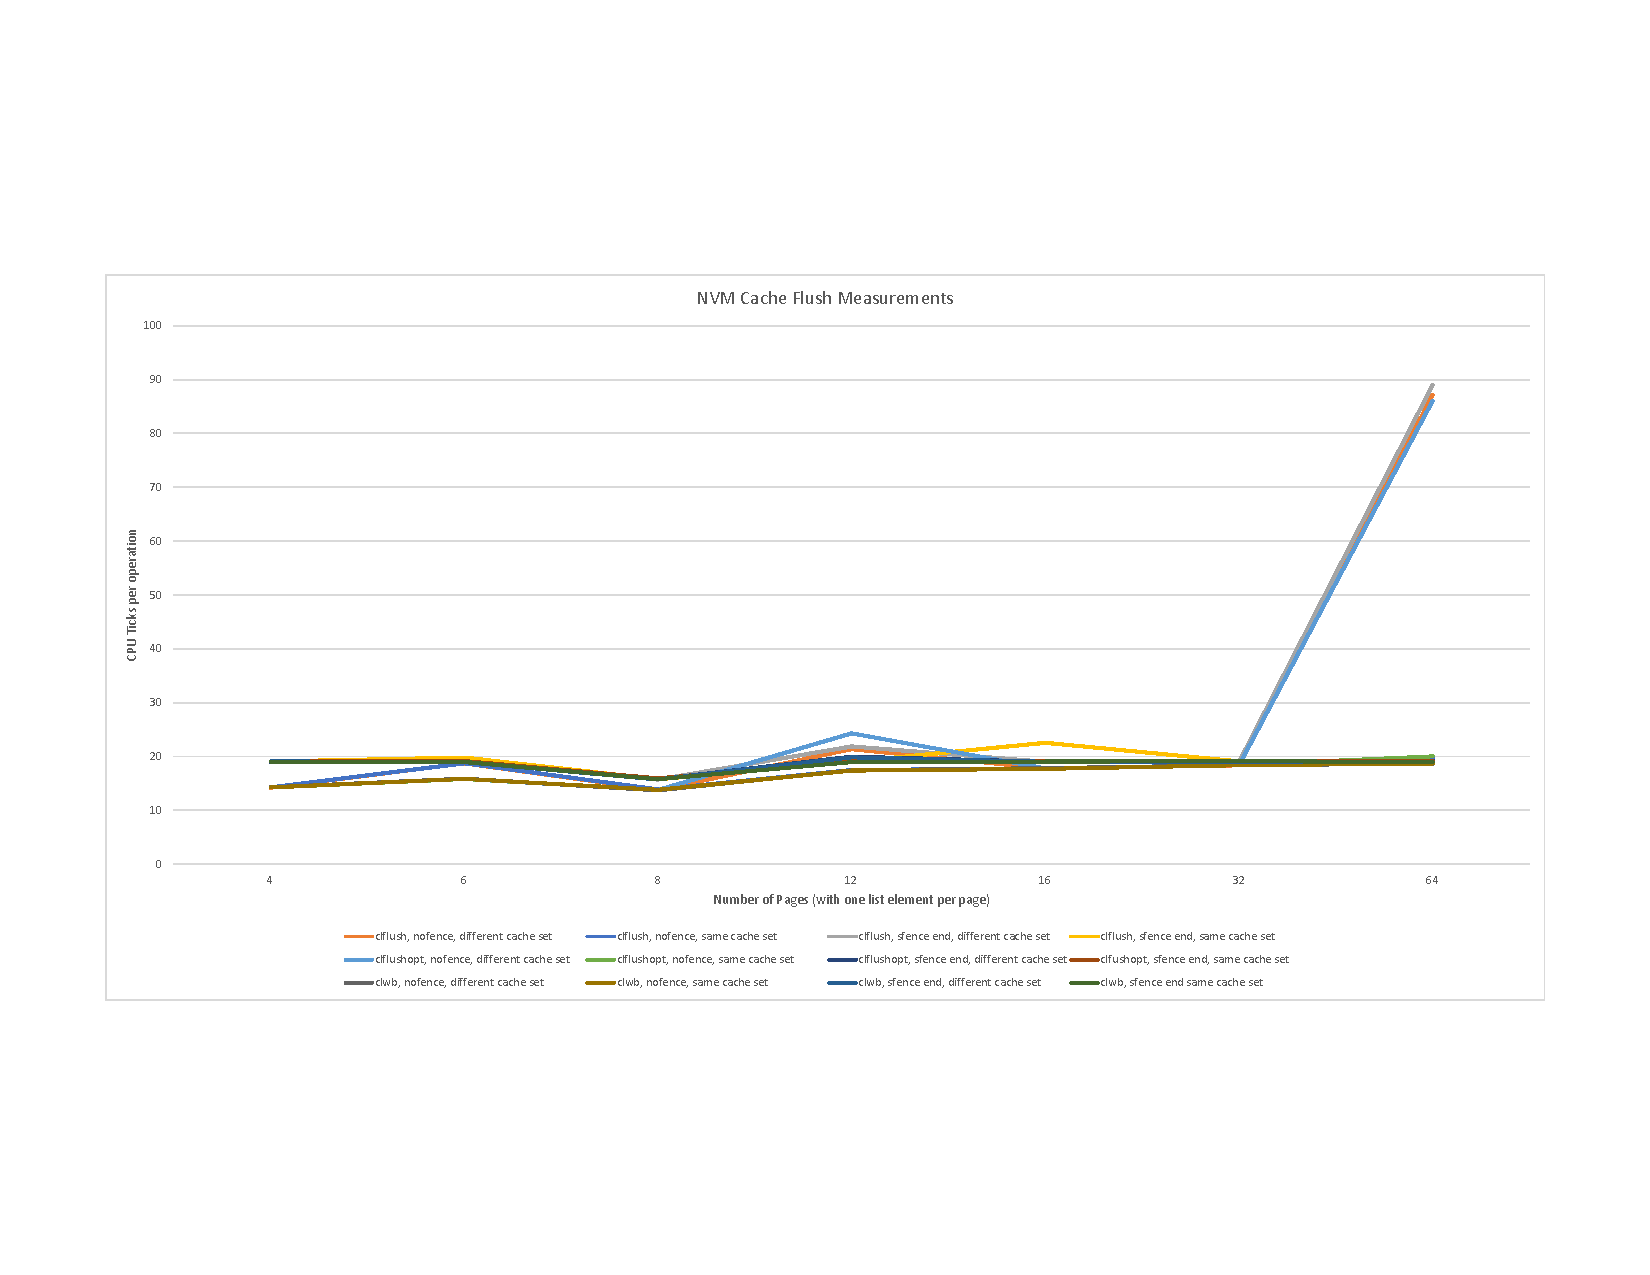
\includegraphics[scale=0.35]{micro/nvm-cache-flush-measurements.pdf}
\end{figure}

These tests work by creating linked list entries from a pool
of memory pages.  Each list entry is at the same offset within
the page, which causes them to be assigned to the same CPU
associative cache set. 

For example, the following code was used for testing clflush
without fencing (Figure \ref{micro:cache-flush}):

%\begin{minted}{c}
\begin{verbatim}
    
static unsigned long test_cache_clflush_nofence(record_page_t *rp)
{
    record_t *r = rp->records[0].s.next;
    unsigned long start, end, time;
    unsigned count = 0;

    time = 0;

    while (r != &rp->records[0]) {
        start = _rdtsc();
        r->s.counter++;
        _mm_clflush(r);
        r = r->s.next;
        end = _rdtsc();
        time += end - start;
        count++;
    }

    // report the amount of CPU time
    return time;

}
\end{verbatim}
%\end{minted}

The goal of this effort was to measure the specific overhead of
the given operation: incrementing the counter, flushing the update, and then advancing to the next record in the list.
Since the list is a circular doubly linked list, this will
access each of the list elements exactly once.  The use of
the pointers confounds the processor prefetch logic, since it
depends upon the value loaded from memory.

The processor tick counter is used for all measurements.  This
can be converted to time based upon the processor speed but I
chose to use ticks for this analysis (the two should be 
equivalent.)

All of the tests are modeled after similar behavior, where
timings are collected around specific operations and attempt
to ignore the overhead of the test harness.

The interesting insight in these results is that the \textbf{non-flushed} paths experience
a substantial penalty once the number of entries in a linked 
list reach 64 unique entries.  This is interesting because the
internal memory controller has 56 write back buffers (this is
for Skylake Xeon processors).


\subsection{CLFLUSHOPT}\label{micro:sec:clflushopt}

The \texttt{clflushopt} instruction was introduced by Intel to provide a mechanism for writing back a single cache line, unlike
the earlier \texttt{clflush} instruction. This instruction
invalidates the given cache line.  A subsequent \texttt{sfence}
guarantees that the cache line is persistent.

This instruction is present on current generation Intel CPUs,
but is not present on older CPUs.

Note that \texttt{clflushopt} may be executed in parallel with
other \texttt{clflushopt} instructions within the same
instruction stream (e.g., parallel execution is permissible).

\subsubsection{Different Cache Set}\label{impl:mb:clflushopt:diffset}
\begin{figure}
    \centering
    \caption{NVM CLFLUSHOPT (Different CPU Set)}\label{micro:clflushopt:different}
    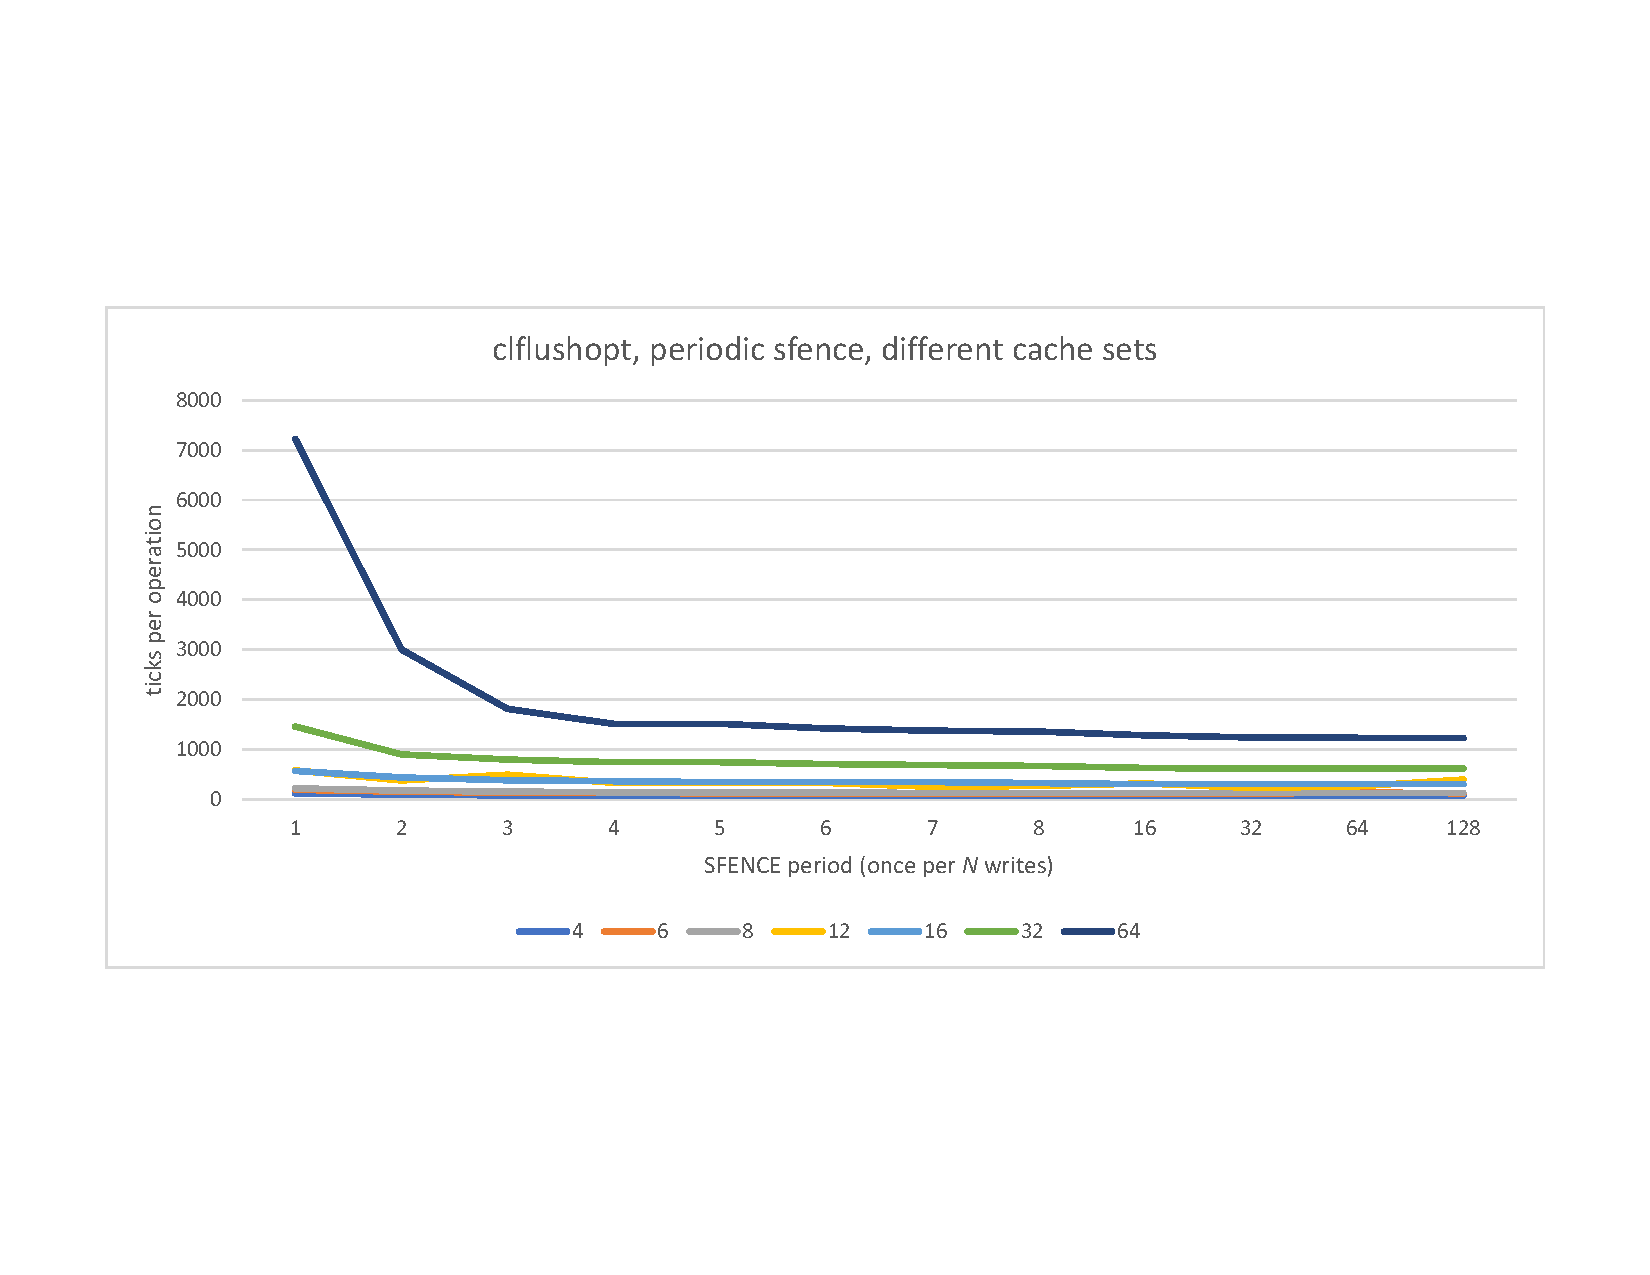
\includegraphics[scale=0.35]{micro/nvm-clflushopt-periodic-different.pdf}
\end{figure}

These results are shown in in Figure 
\ref{micro:clflushopt:different}.

There is a notable improvement in performance when the sfence operation period is decreased; for this test there is minimal improvement doing it less frequently than once per four write operations.

\subsubsection{Same Cache Set}\label{impl:mb:clflushopt:sameset}

\begin{figure}
    \centering
    \caption{NVM CLFLUSHOPT (Same CPU Set)}\label{micro:clflushopt:same}
    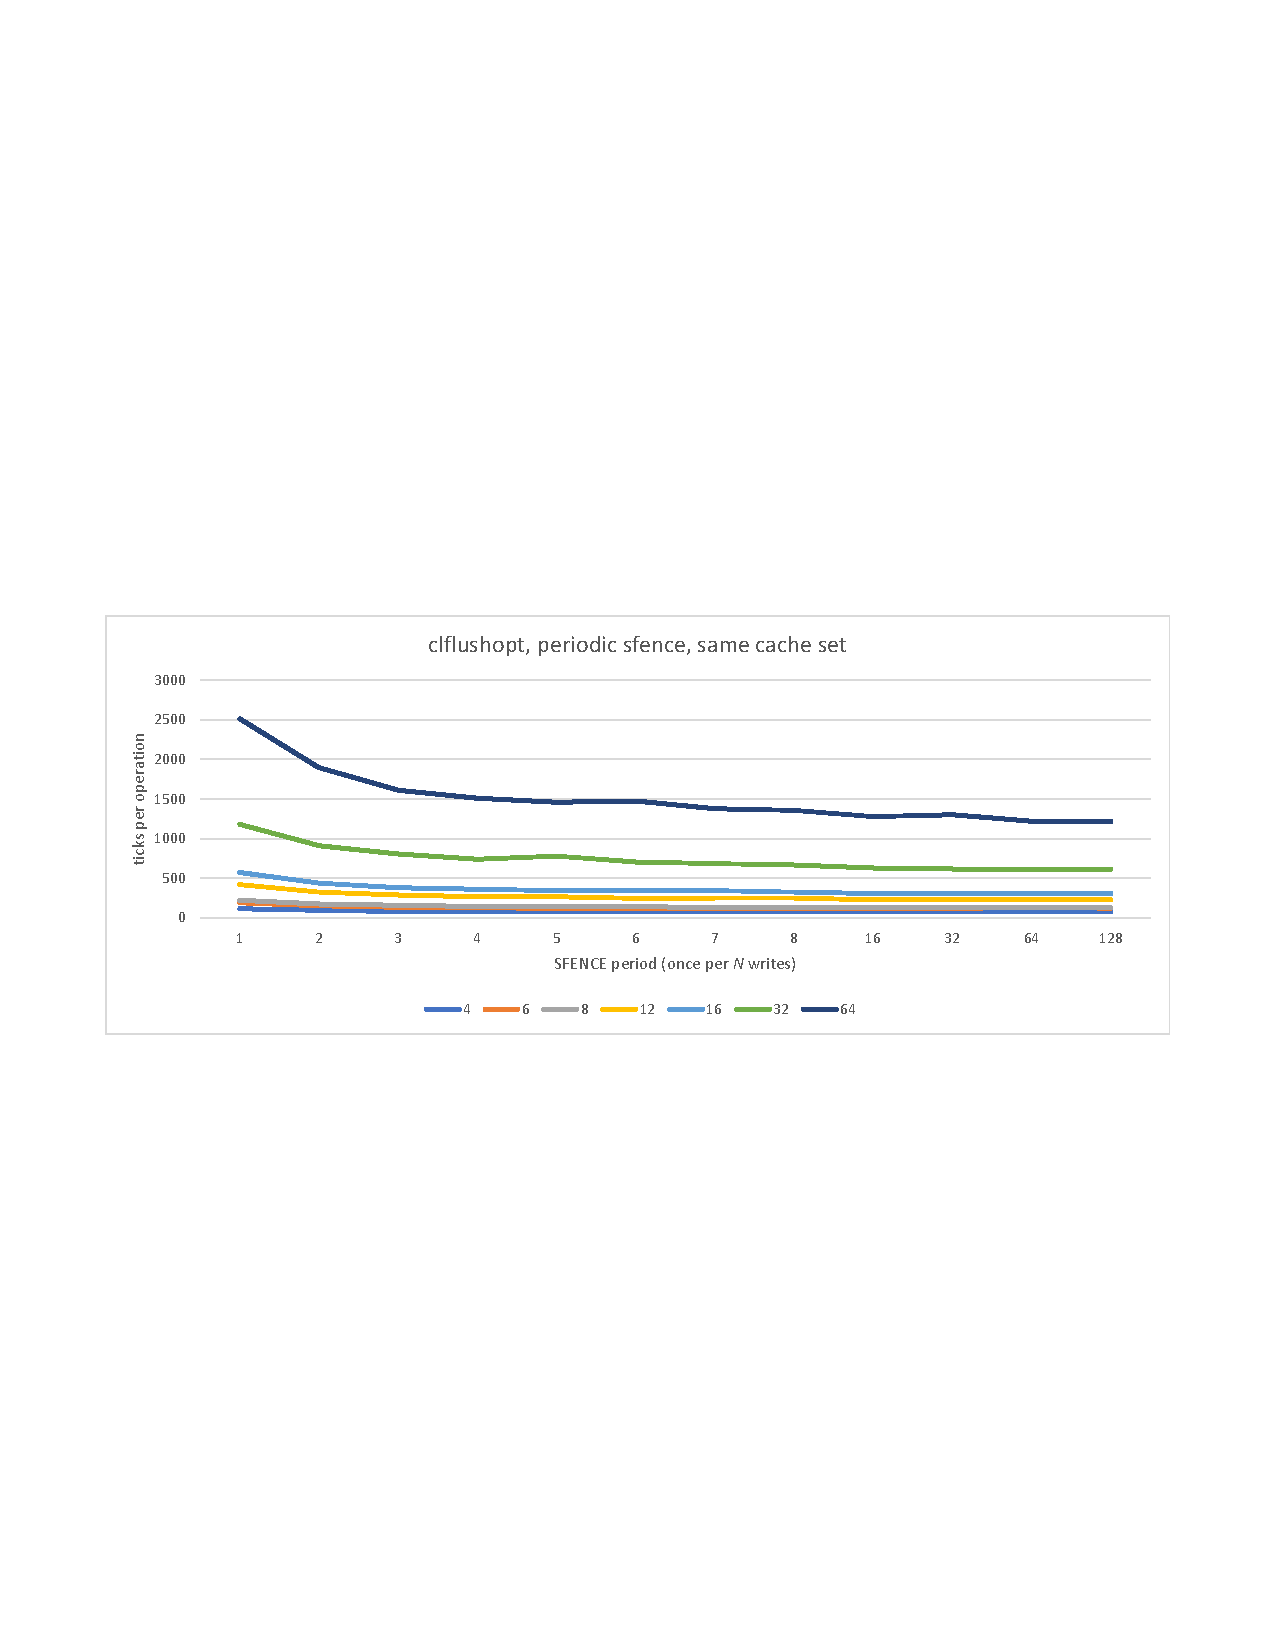
\includegraphics[scale=0.35]{micro/nvm-clflushopt-periodic-same.pdf}
\end{figure}

These results are shown in Figure \ref{micro:clflushopt:same}.

There is a notable improvement in performance when the sfence operation period is decreased; for this test there is minimal improvement doing it less frequently than once per four write operations.


\section{CLFUSH}\label{micro:sec:clflush}

The \texttt{clflush} processor instruction on Intel CPUs
causes a flush back of the specified cache line.  It is
distinct from \texttt{clflushopt} in that it is serialized
with respect to other \texttt{clflush} instructions on the same core.

There are suggestions from observed behavior that some
implementations of \texttt{clflush} may cause flushing of
other cache contents as well.

\subsection{Different Cache Set}
\begin{figure}
    \centering
    \caption{NVM CLFLUSH (Different CPU Set)}\label{micro:clflush:different}
    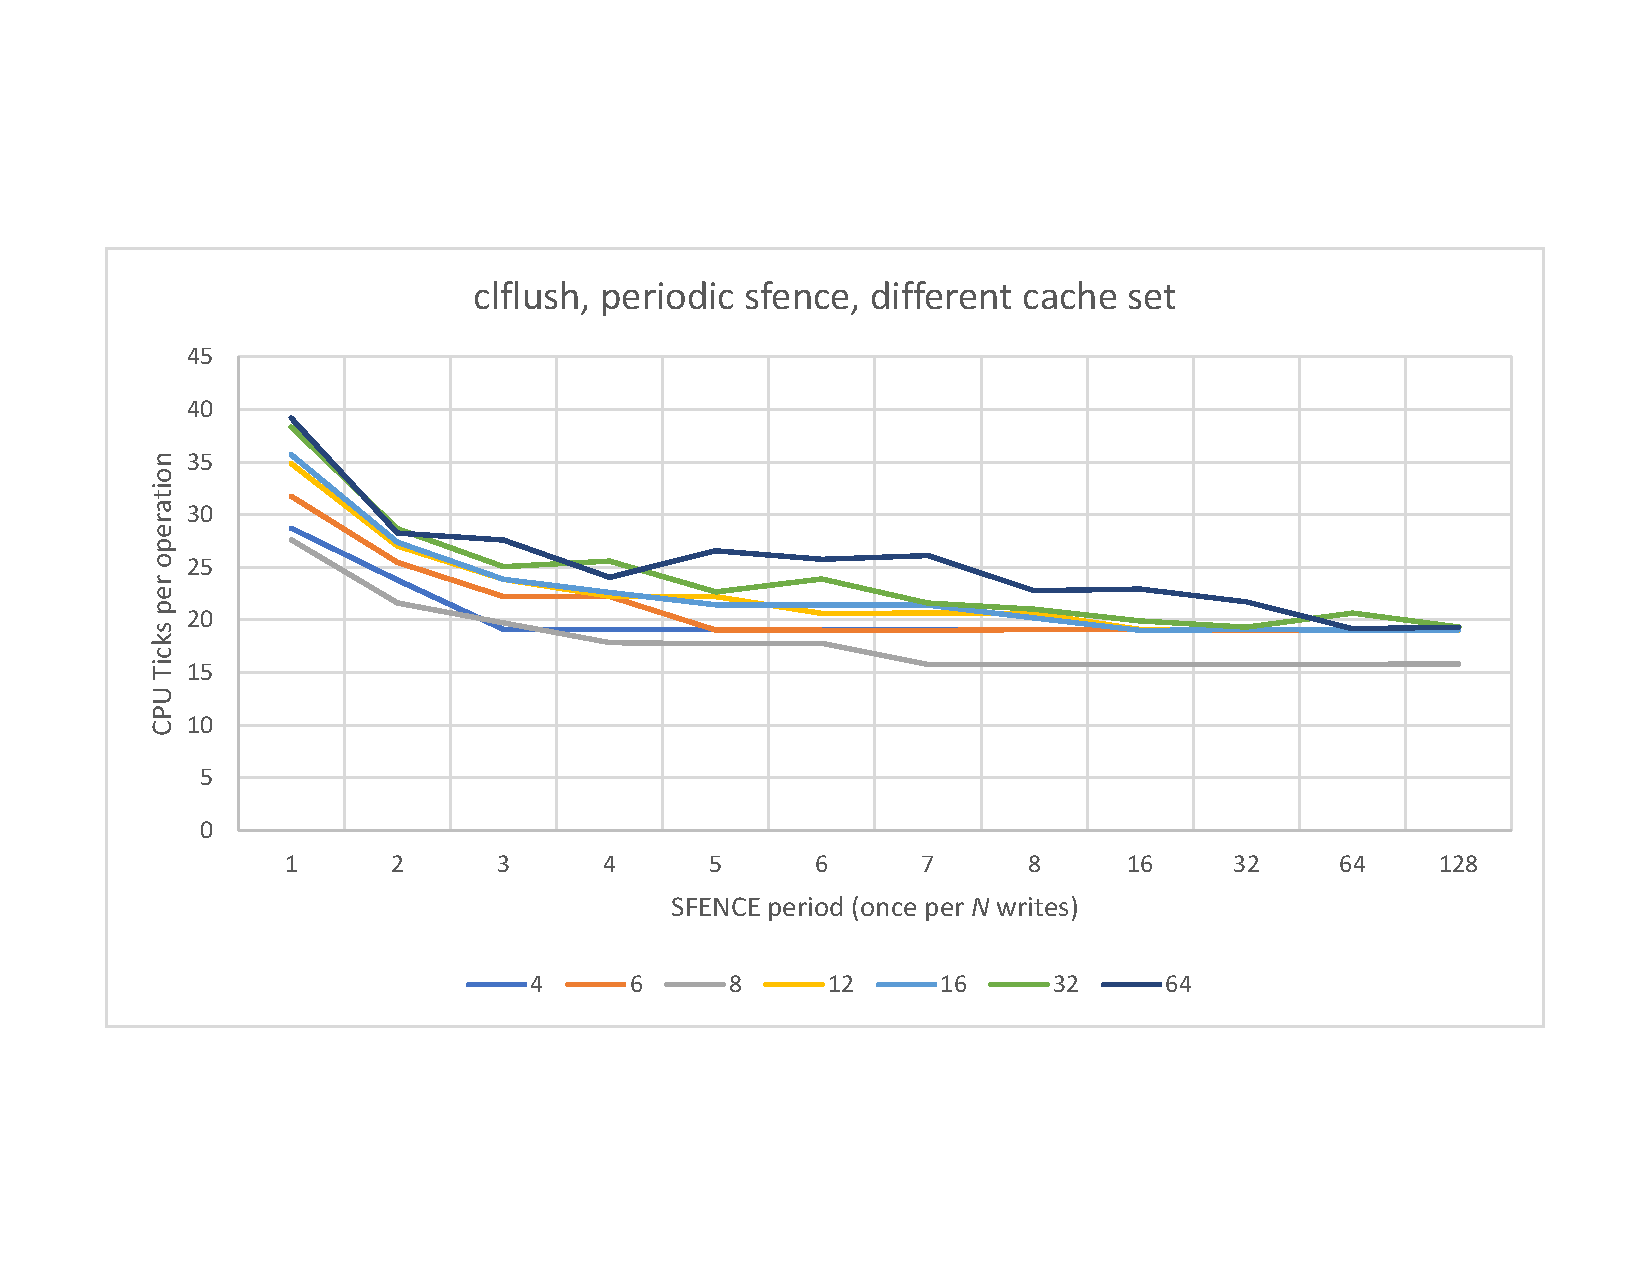
\includegraphics[scale=0.35]{micro/nvm-clflush-periodic-different.pdf}
\end{figure}

These results are shown in Figure \ref{micro:clflush:different}.

The behavior, shown in Figure \ref{micro:clflush:different},
is similar to the behavior observed previously with the
\texttt{clfushopt} instruction (\S \ref{micro:sec:clflushopt}).

The behavior is not entirely smooth, unlike what I observed
earlier with the \texttt{clflushopt} instruction (\S \ref{micro:sec:clflushopt}).

\subsection{Same Cache Set}

\begin{figure}
    \centering
    \caption{NVM CLFLUSH (Same CPU Set)}\label{micro:clflush:same}
    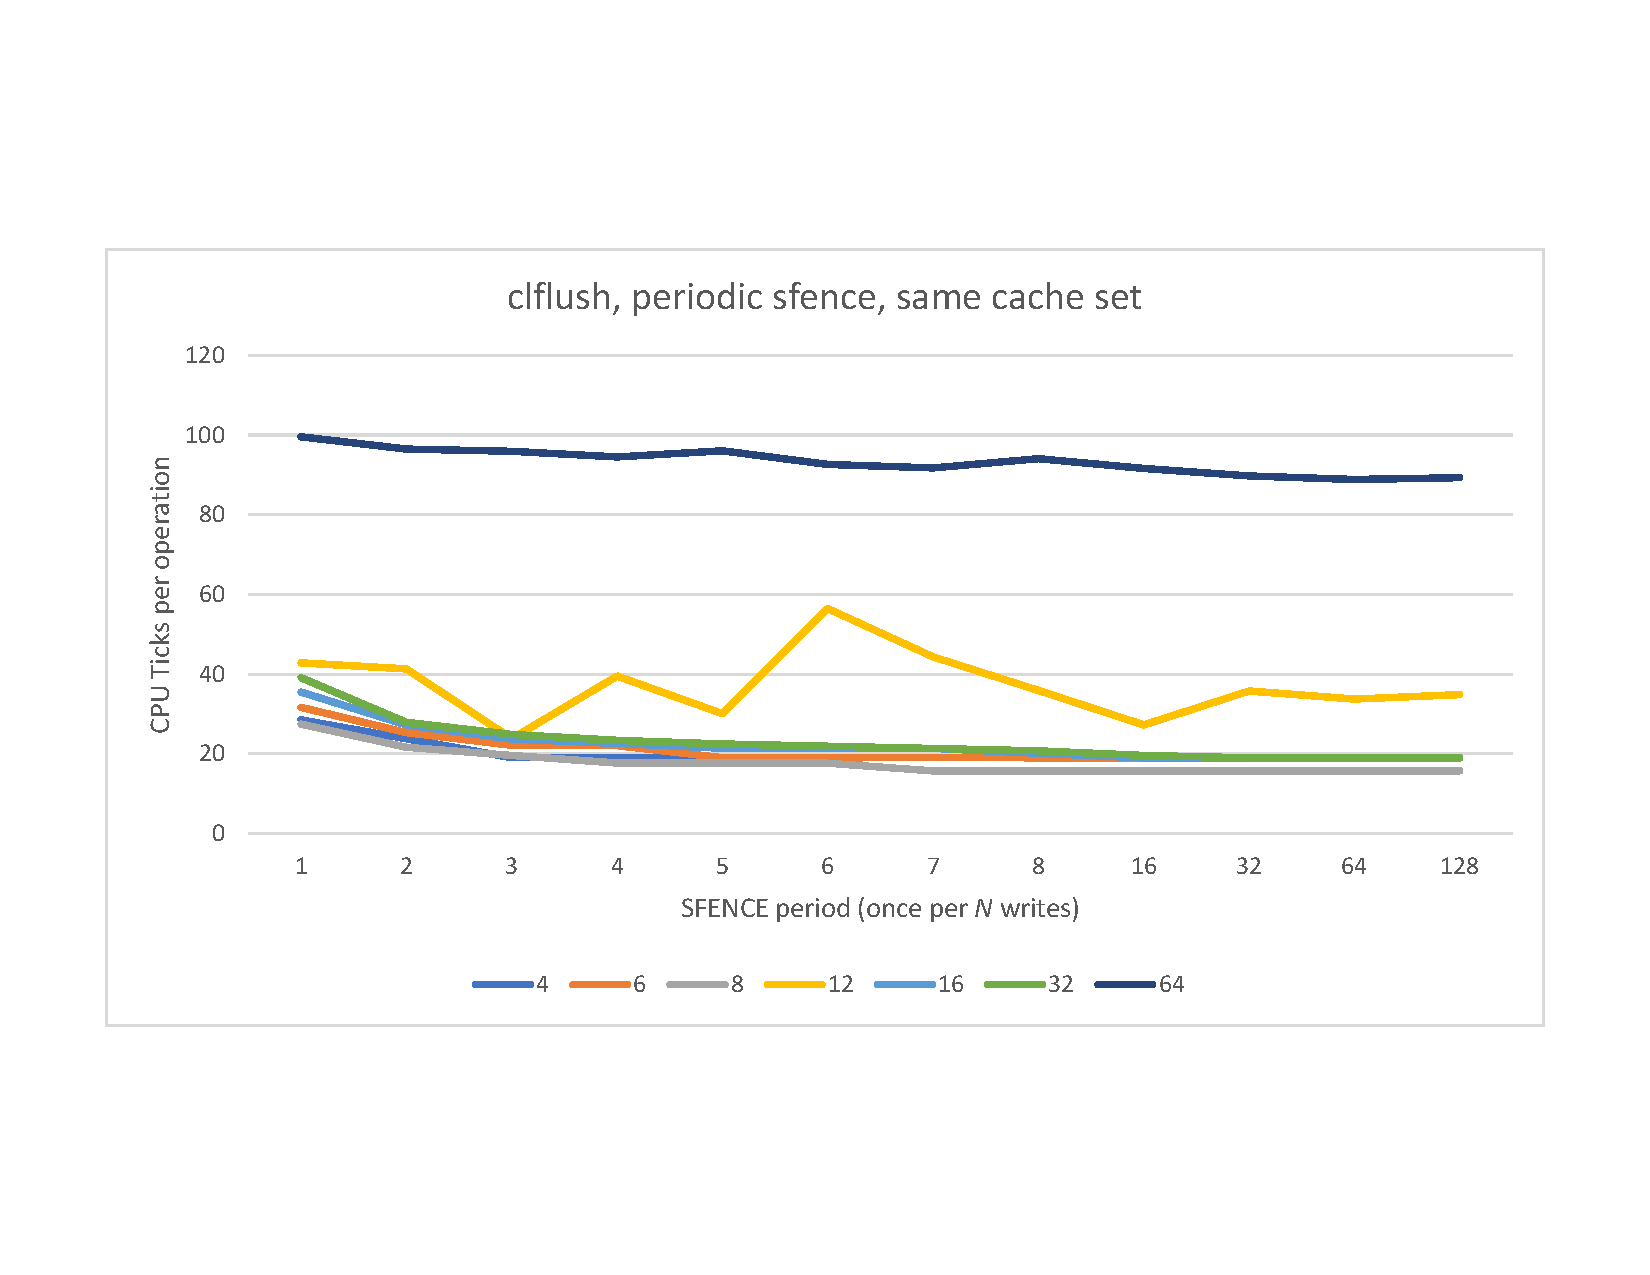
\includegraphics[scale=0.35]{micro/nvm-clflush-periodic-same.pdf}
\end{figure}

These results are shown in Figure \ref{micro:clflush:same}.

The interesting observation for this test is that it shows an improvement similar to what was seen with \texttt{clflushopt} (See \S \ref{micro:sec:clflushopt}).  However, unlike the
previous result, this one is not as smooth or consistent. This
may be a benefit of the parallel nature of the \texttt{clflushopt} instruction.

The other interesting departure from the earlier results is that
this shows a notable \textbf{penalty} for the large size set.
The reason for this is not clear from this data; further work
may be required.

Finally, when comparing the two different cache set patterns, I
observed that the best performance appears to be for the list
of size eight. It is not clear to me why this would be the case.

\section{CLWB}\label{micro:sec:clwb}

The \texttt{clwb} instruction has been recently added in the 
Intel Skylake Server class CPUs.  It enhances the behavior of
the previous \texttt{clflushopt} instruction by not
evicting the cache line from the set --- this \textit{writes}
data back but does not cause it to be evicted from the cache.

This instruction is useful for data structures that require
updating over time, such as counters or various kinds of
table structures.

This instruction is expected to be present in future Intel processors.

\subsection{Different Cache Set}

\begin{figure}
    \centering
    \caption{NVM CLWB (Different CPU Set)}\label{micro:clwb:different}
    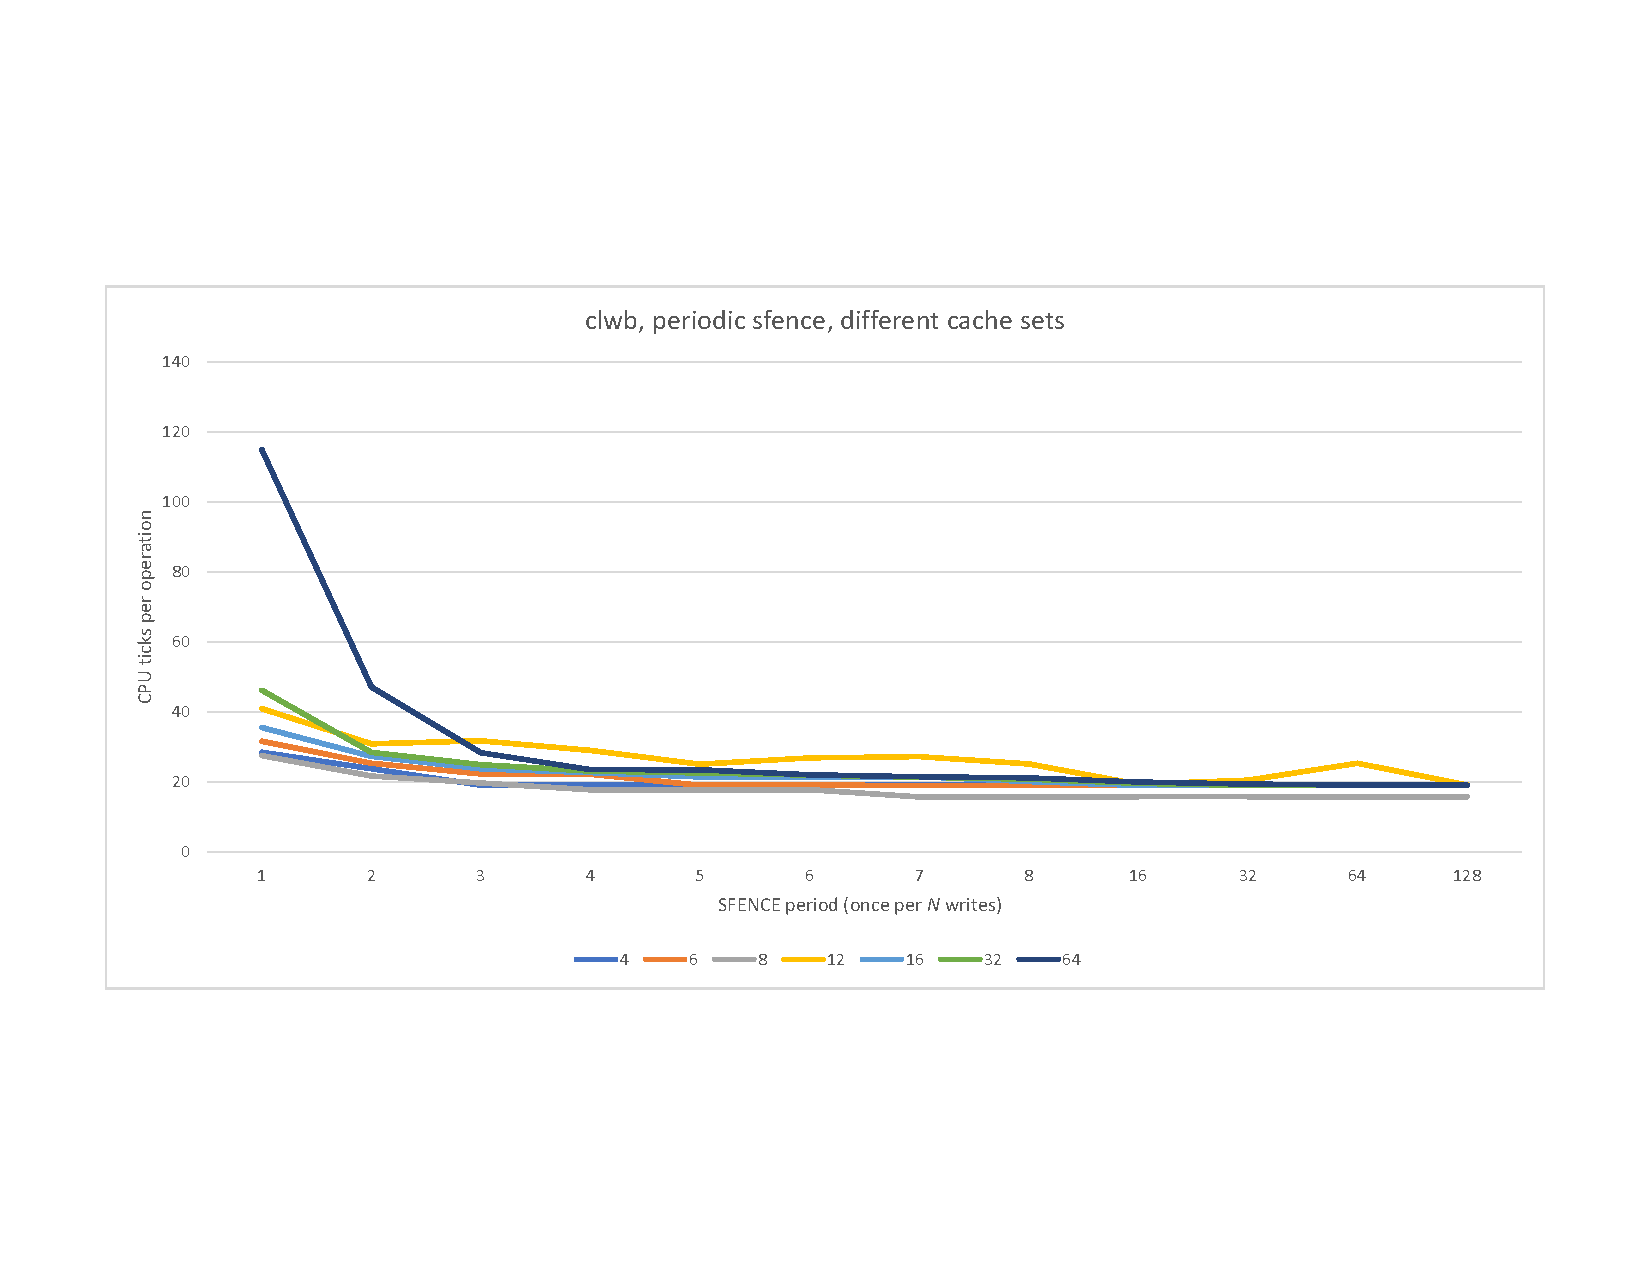
\includegraphics[scale=0.35]{micro/nvm-clwb-periodic-different.pdf}
\end{figure}

These results are shown in Figure \ref{micro:clwb:different}.

The performance here is similar to that which I observed
using the other flush operations --- \texttt{clflushopt} (\S \ref{micro:sec:clflushopt}) and \texttt{clflush} (\S \ref{micro:sec:clflush}).

There are some interesting observations from this data: the 64 entry long linked list set shows very poor performance when combined with aggressive fence operations, but converges towards the mean for less aggressive fence operations.

Much like I previously noted (\S \ref{micro:sec:clflush}),
it is interesting that the list of length 8 again has consistently better performance for most periodic fencing operation counts.

\subsection{Same Cache Set}

\begin{figure}
    \centering
    \caption{NVM CLWB (Same CPU Set)}\label{micro:clwb:same}
    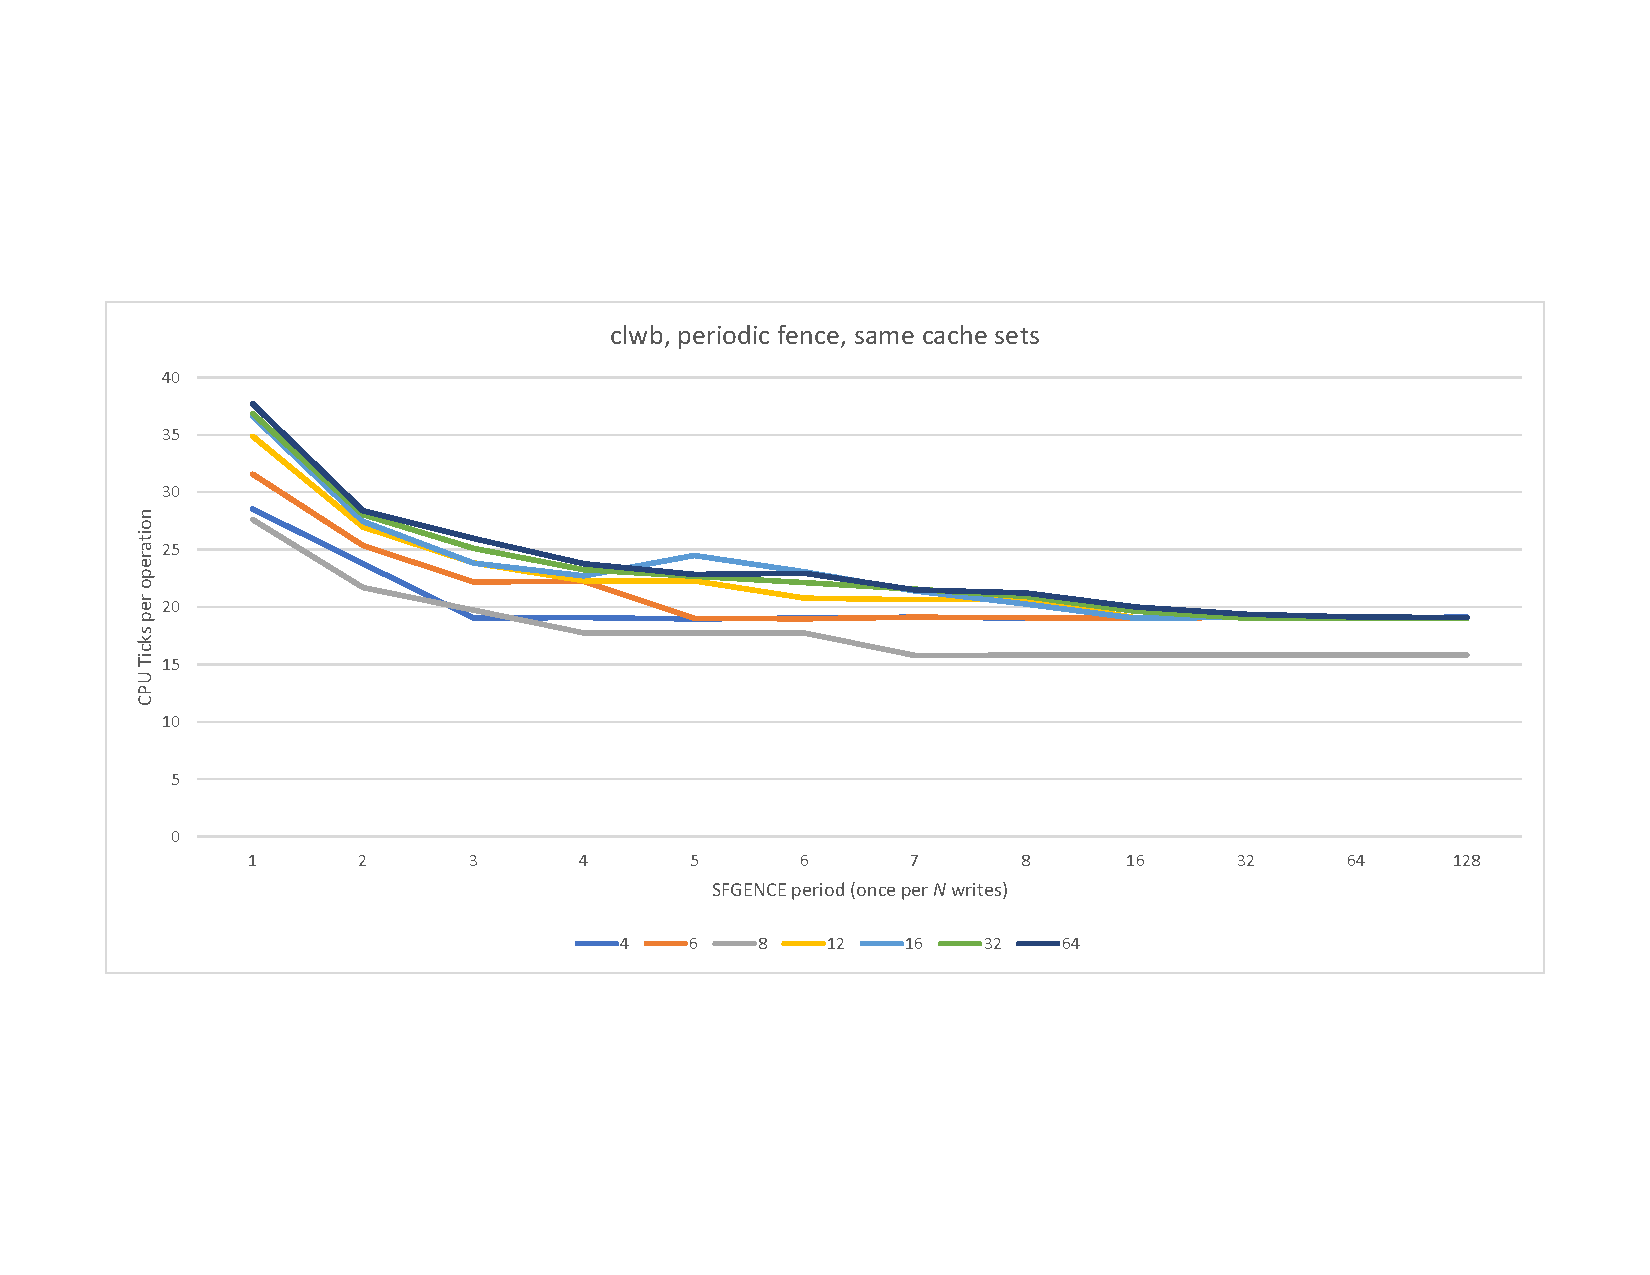
\includegraphics[scale=0.35]{micro/nvm-clwb-periodic-same.pdf}
\end{figure}

These results are shown in Figure \ref{micro:clwb:same}.

Two observations: every linked list set \textit{other than} the
eight entry list converges to the same performance (approximately 19 clock ticks).  The 8 entry list converges just under 16 ticks.  This 20\% difference (which I observed previously, see \S \ref{micro:sec:clflush} and \S \ref{micro:sec:clflushopt}) seems to
be fairly consistent throughout the various tests. 

\section{Linked List}

The basis for these micro-benchmarks is a circular doubly
linked list structure.  In this section I have evaluated the
performance of those without utilizing cache flushing primitives,
though I have incorporated fencing operations in these
measurements.

\subsection{No Flush}\label{ll:sec:noflush}

\begin{figure}
    \centering
    \caption{NVM Linked List Baseline (No Flush)}\label{micro:llbaseline:noflush}
    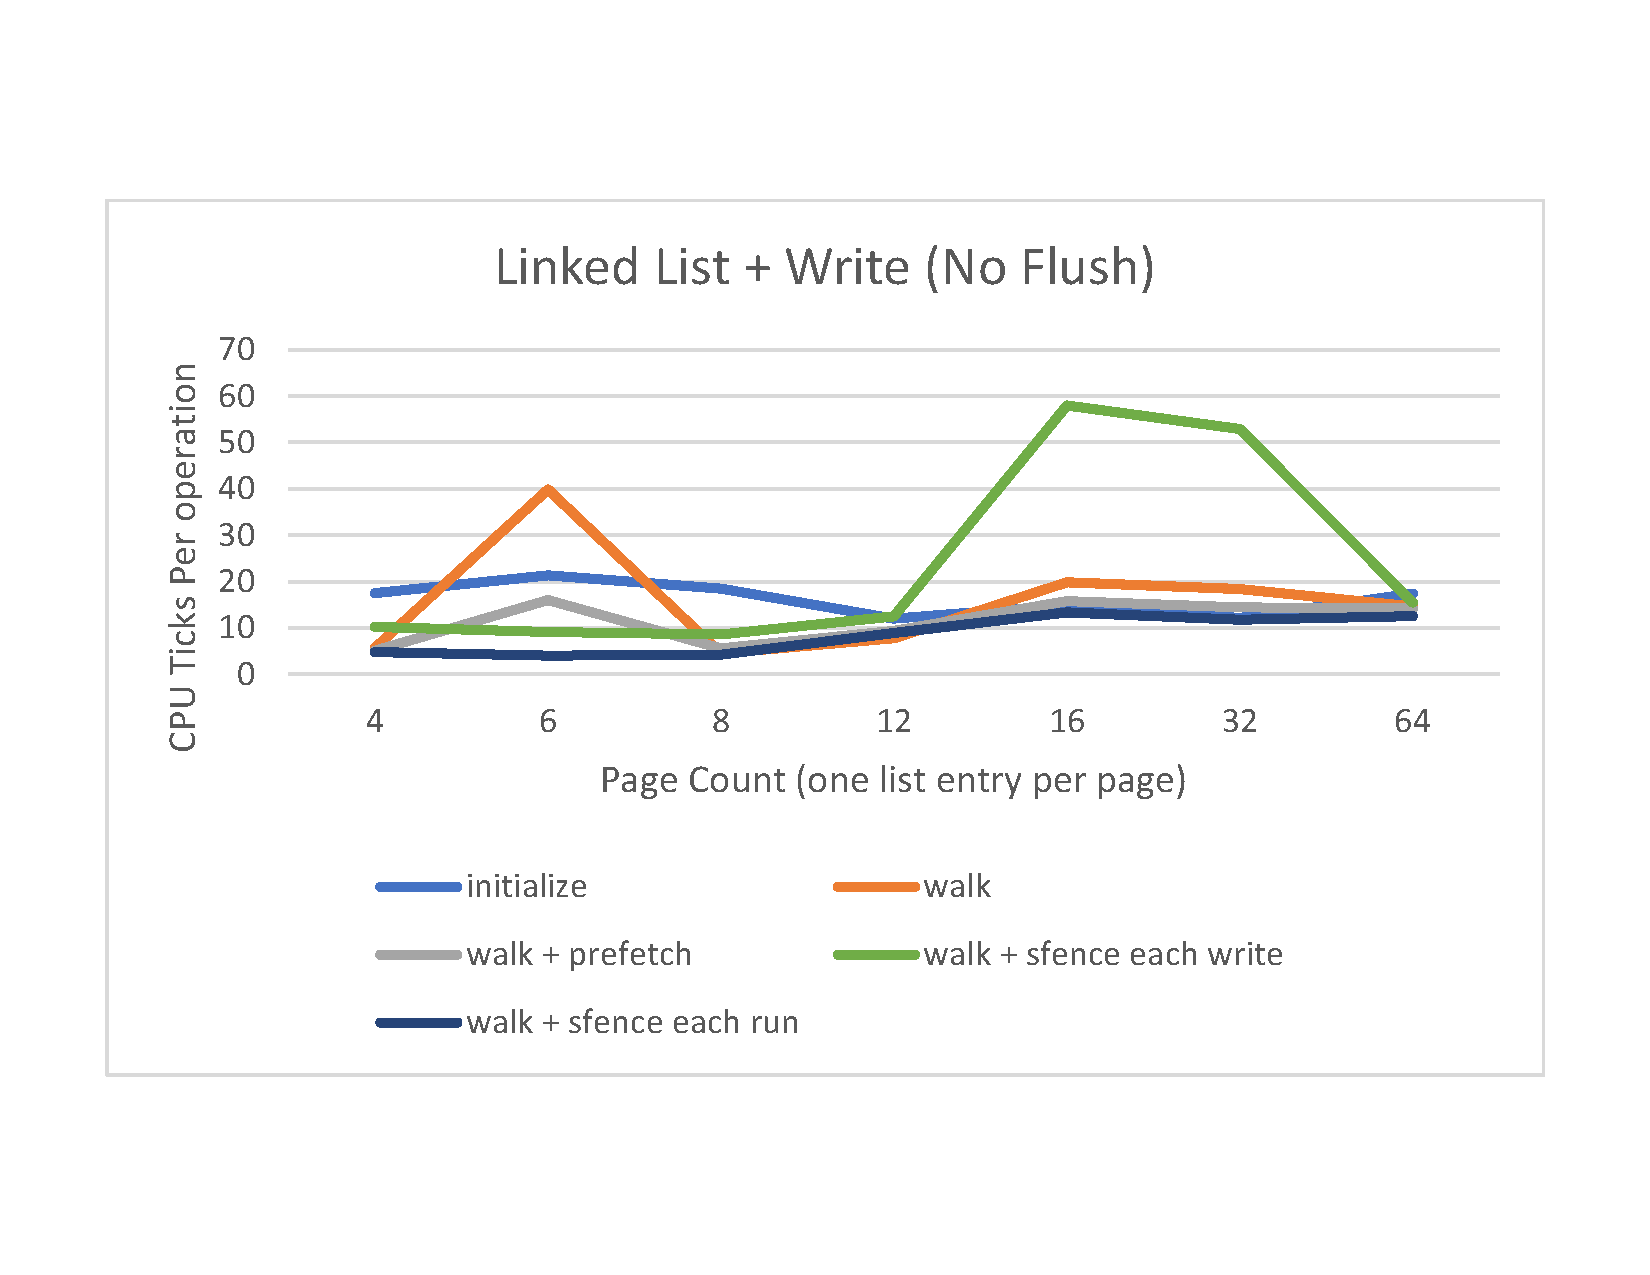
\includegraphics[scale=0.35]{micro/nvm-linked-list-baseline-no-flush.pdf}
\end{figure}

The results for the linked list test without flushing is
shown in Figure \ref{micro:llbaseline:noflush}.

Note that these tests are all from the same cache set.

The test looks at five different scenarios:

\begin{description}
    \item[initialize] --- this is the performance of the list initialization code.  It takes the first 64 byte block of each page given and initializes it to be in a linked list with a zero value for the counter.
    \item[walk] --- this is the cost of walking the list and incrementing the counter.
    \item[walk + prefetch] --- this is where the code prefetches the next pointer value, and walks the list.
    \item[walk + sfence write] --- the code in this case walks, but uses the \texttt{sfence} instruction after each write.
    \item[walk + sfence run] --- the code in this case walks and updates the counter, performing an \texttt{sfence} operation at the end of the entire run (so once per list traversal).
\end{description}

The best overall walk performance came from using an 
\texttt{sfence} operation at the end of each run.  The worst
walk performance was from using an \texttt{sfence} operation
after each write.

These were early results and encouraged me to look at further
cache/flush behaviors.

\subsection{Flush}

\begin{figure}
    \centering
    \caption{NVM Linked List Baseline (With Flush)}\label{micro:llbaseline:flush}
    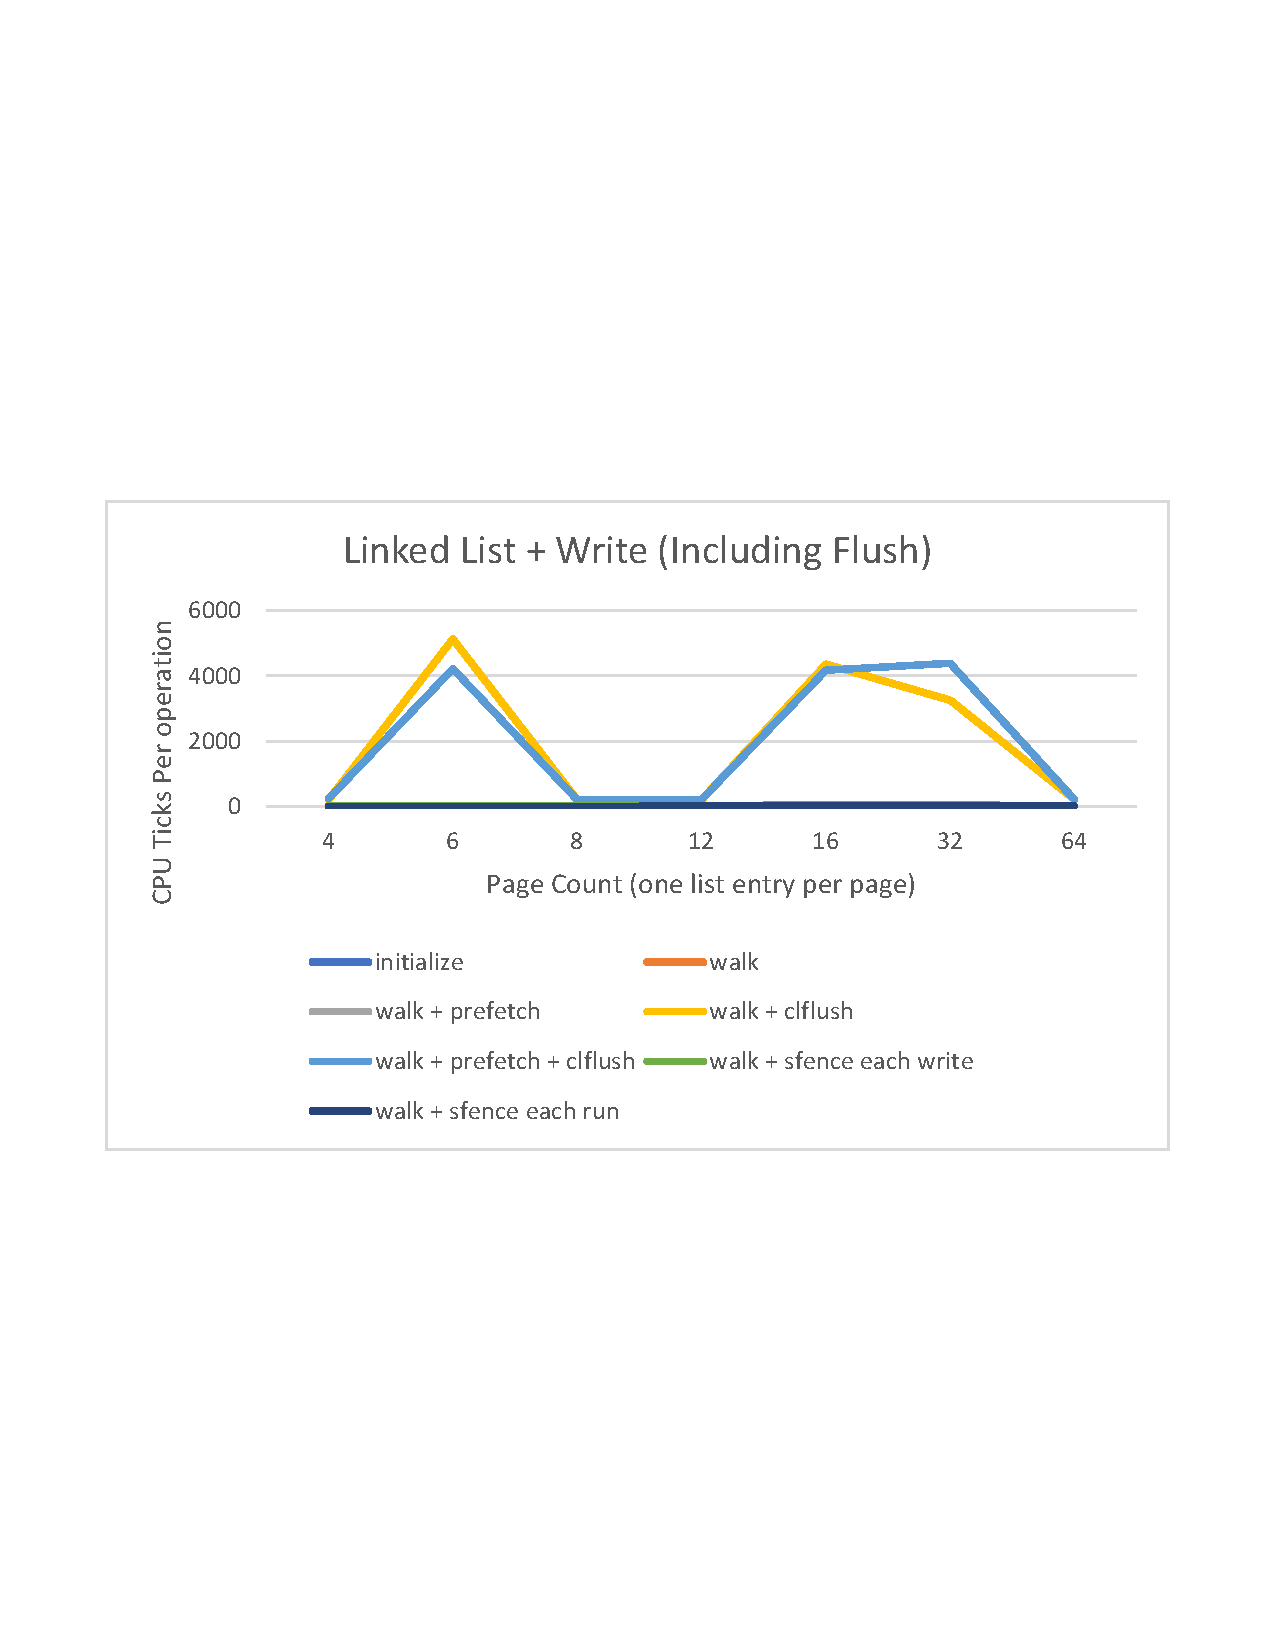
\includegraphics[scale=0.35]{micro/nvm-linked-list-baseline-with-flush.pdf}
\end{figure}

The results for the linked list test with flushing is
shown in Figure \ref{micro:llbaseline:noflush}.

Note that these tests are all from the same cache set.

In addition to the five scenarios described in \S 
\ref{ll:sec:noflush} I added two flushing scenarios.  The
results are shown in Figure \ref{micro:llbaseline:flush}.

The additional scenarios are:

\begin{description}
    \item[walk + clflush] --- the code walks the list and incrementing the counter, with a \texttt{clflush} after each write.
    \item[walk + prefetch + clflush] --- this is where the code prefetches the next pointer value, and walks the list, incrementing the counter, with a \texttt{clflush} after each write.
\end{description}

These results surprised me because the cost associated with
doing a cache flush seemed to be difficult to predict or control. While all seven tests are represented, the cost associated with the flushing operations causes them to be
lost.

\subsection{Periodic Fence}

Evolving from the simple fencing, I broadened my analysis to include periodic fencing.  This section describes those measurements.  In this case there is no flushing.  This helps understand the cost of fence operations. 



\subsubsection{Different Cache Set}

\begin{figure}
    \centering
    \caption{NVM Periodic Fence, No Flush, Different Cache Set}\label{micro:sfence:noflush:different}
    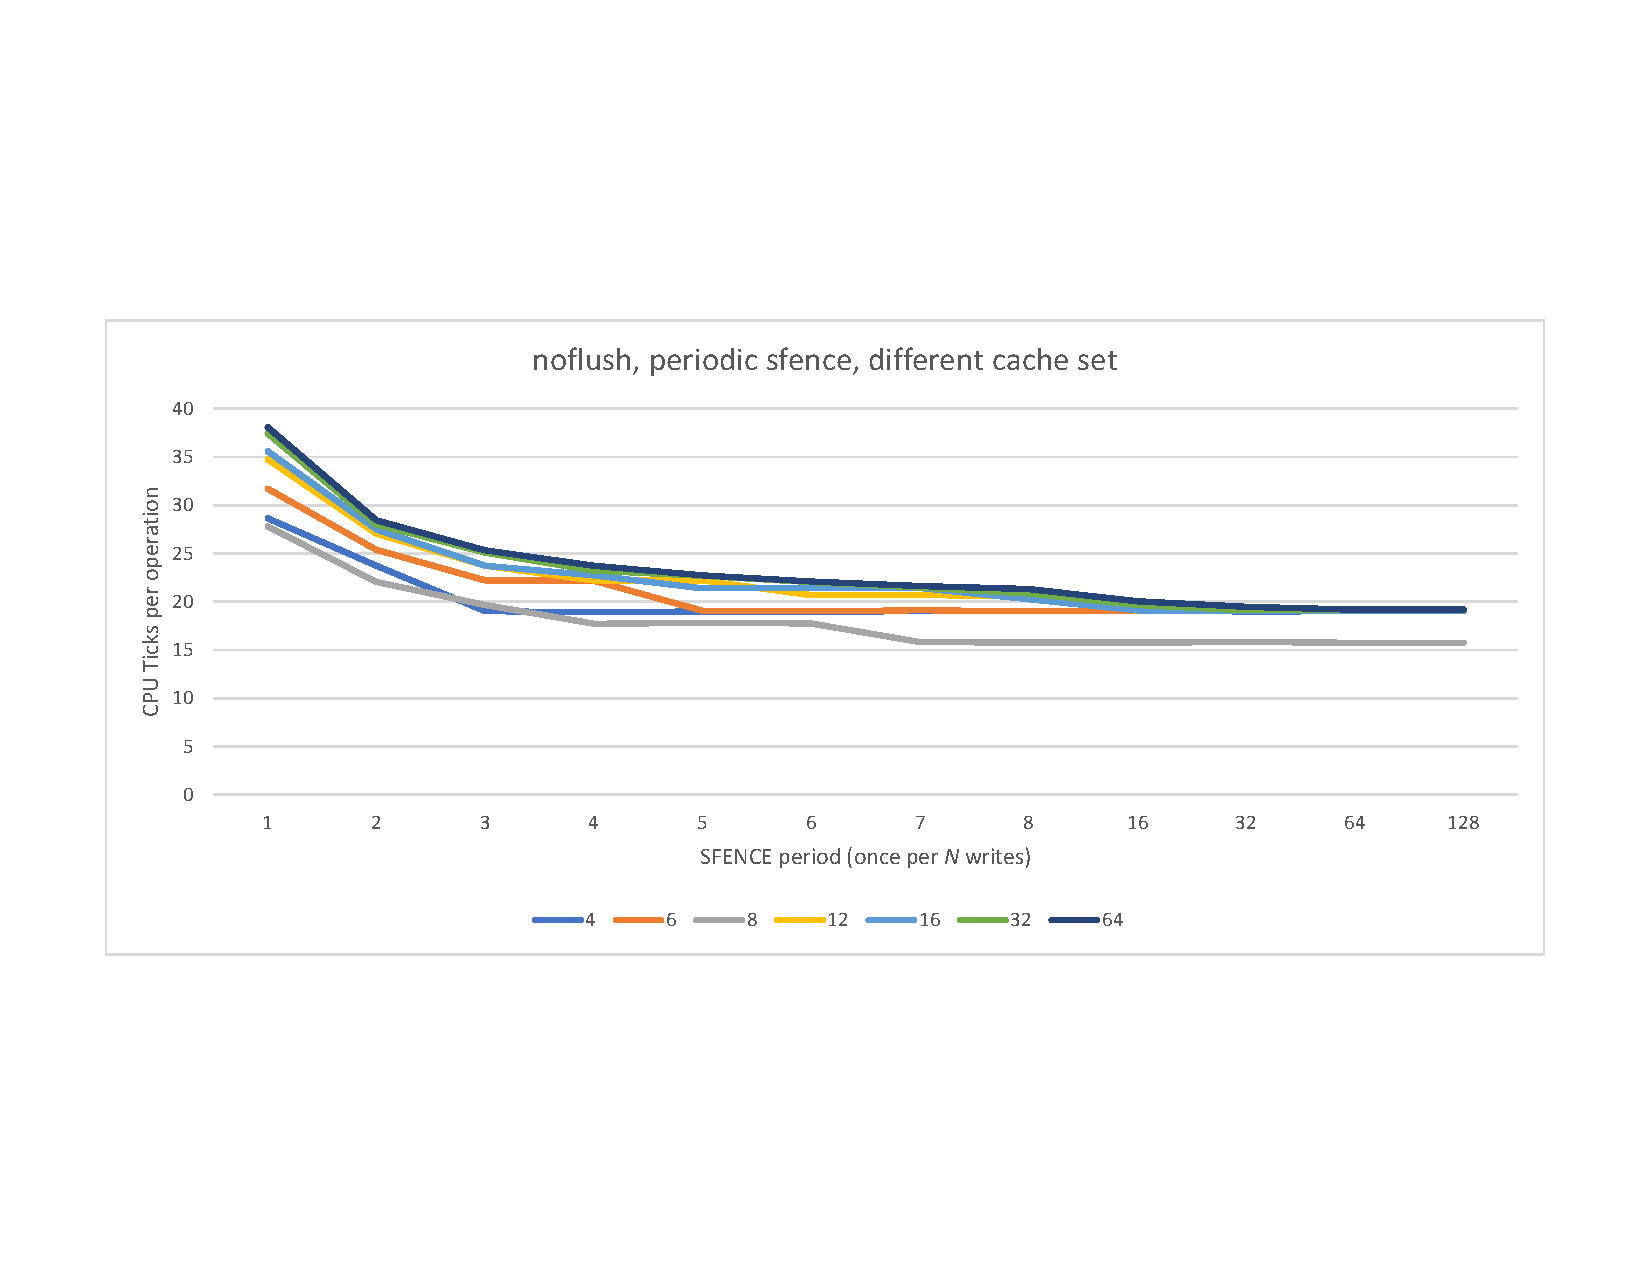
\includegraphics[scale=0.35]{micro/nvm-noflush-periodic-different.pdf}
\end{figure}


\subsubsection{Same Cache Set}

\begin{figure}
    \centering
    \caption{NVM Periodic Fence, No Flush, Same Cache Set}\label{micro:sfence:noflush:same}
    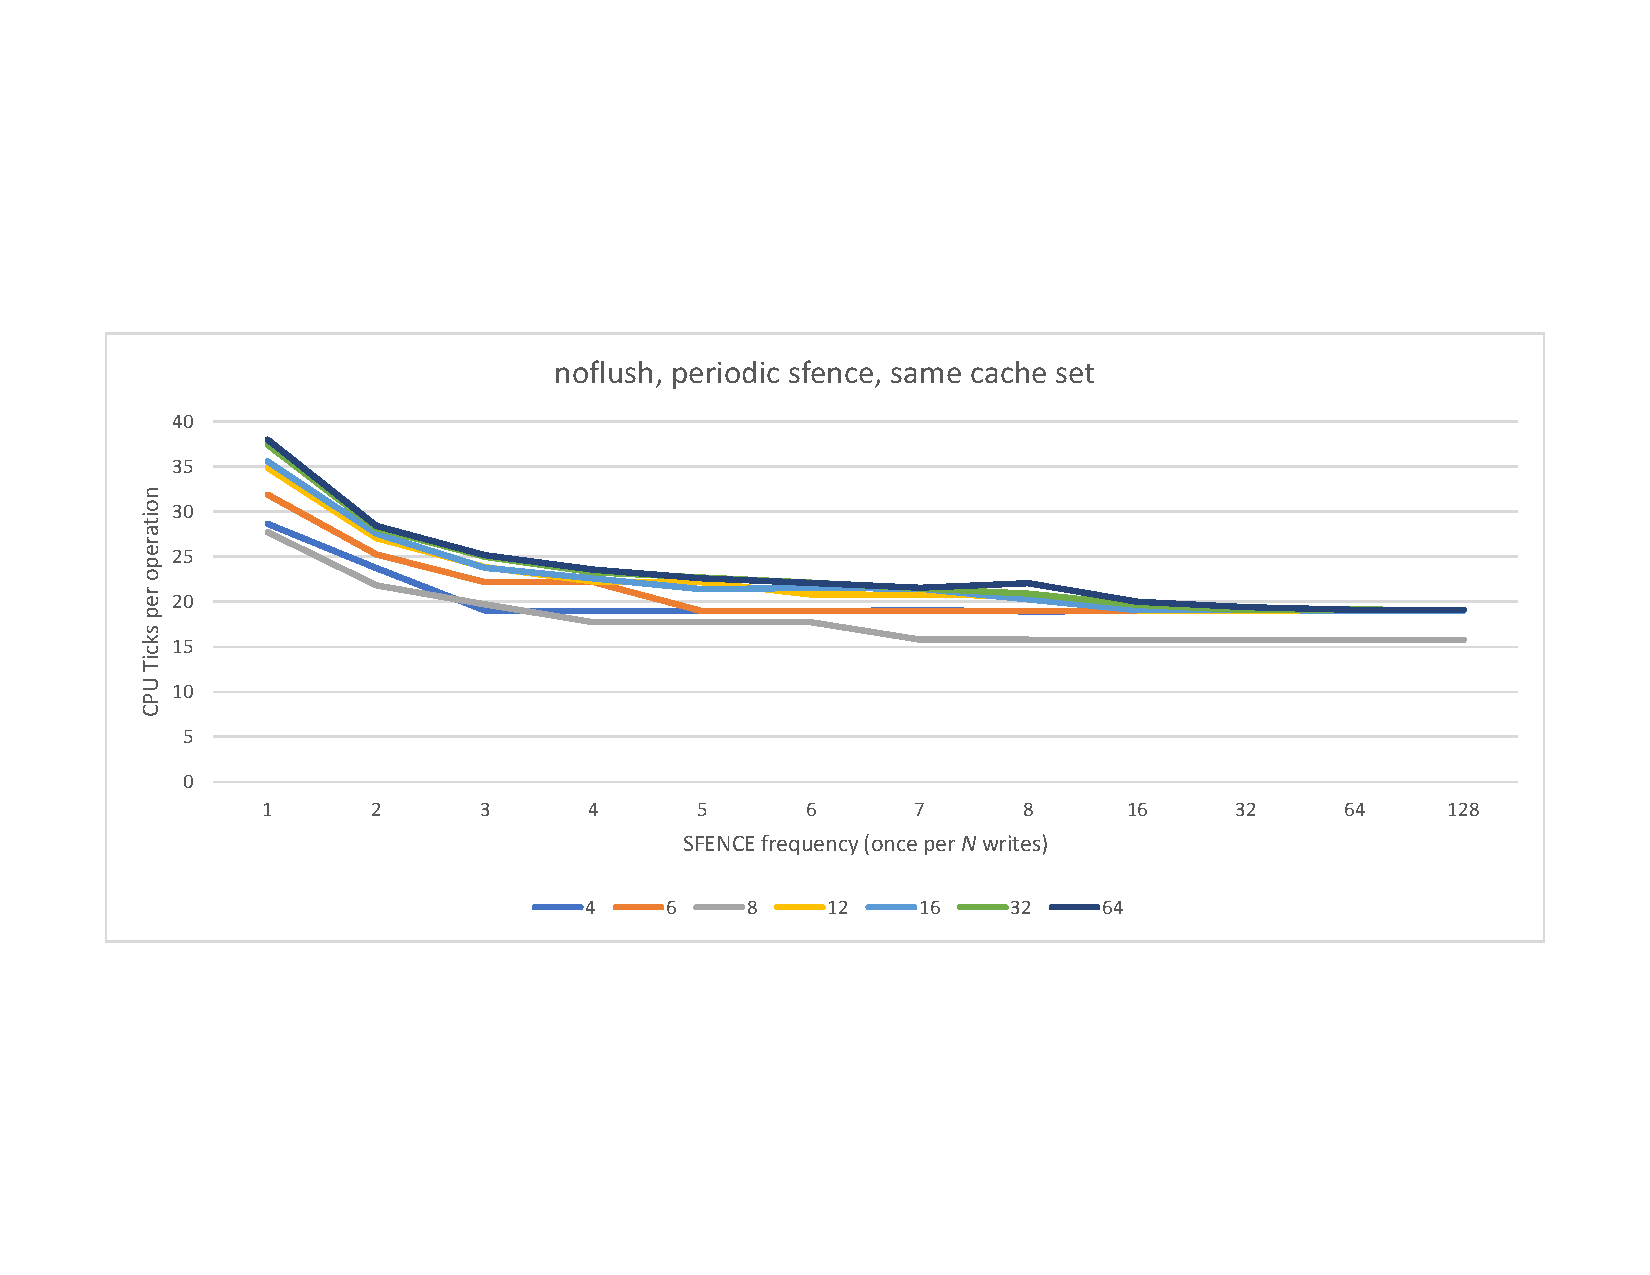
\includegraphics[scale=0.35]{micro/nvm-noflush-periodic-same.pdf}
\end{figure}

\section{Memory Allocator Results}\label{section:results:malloc}

\begin{figure}
    \centering
    \caption{Memory Allocation Tests (Alloc-Free-Alloc)}\label{plot:afa}
    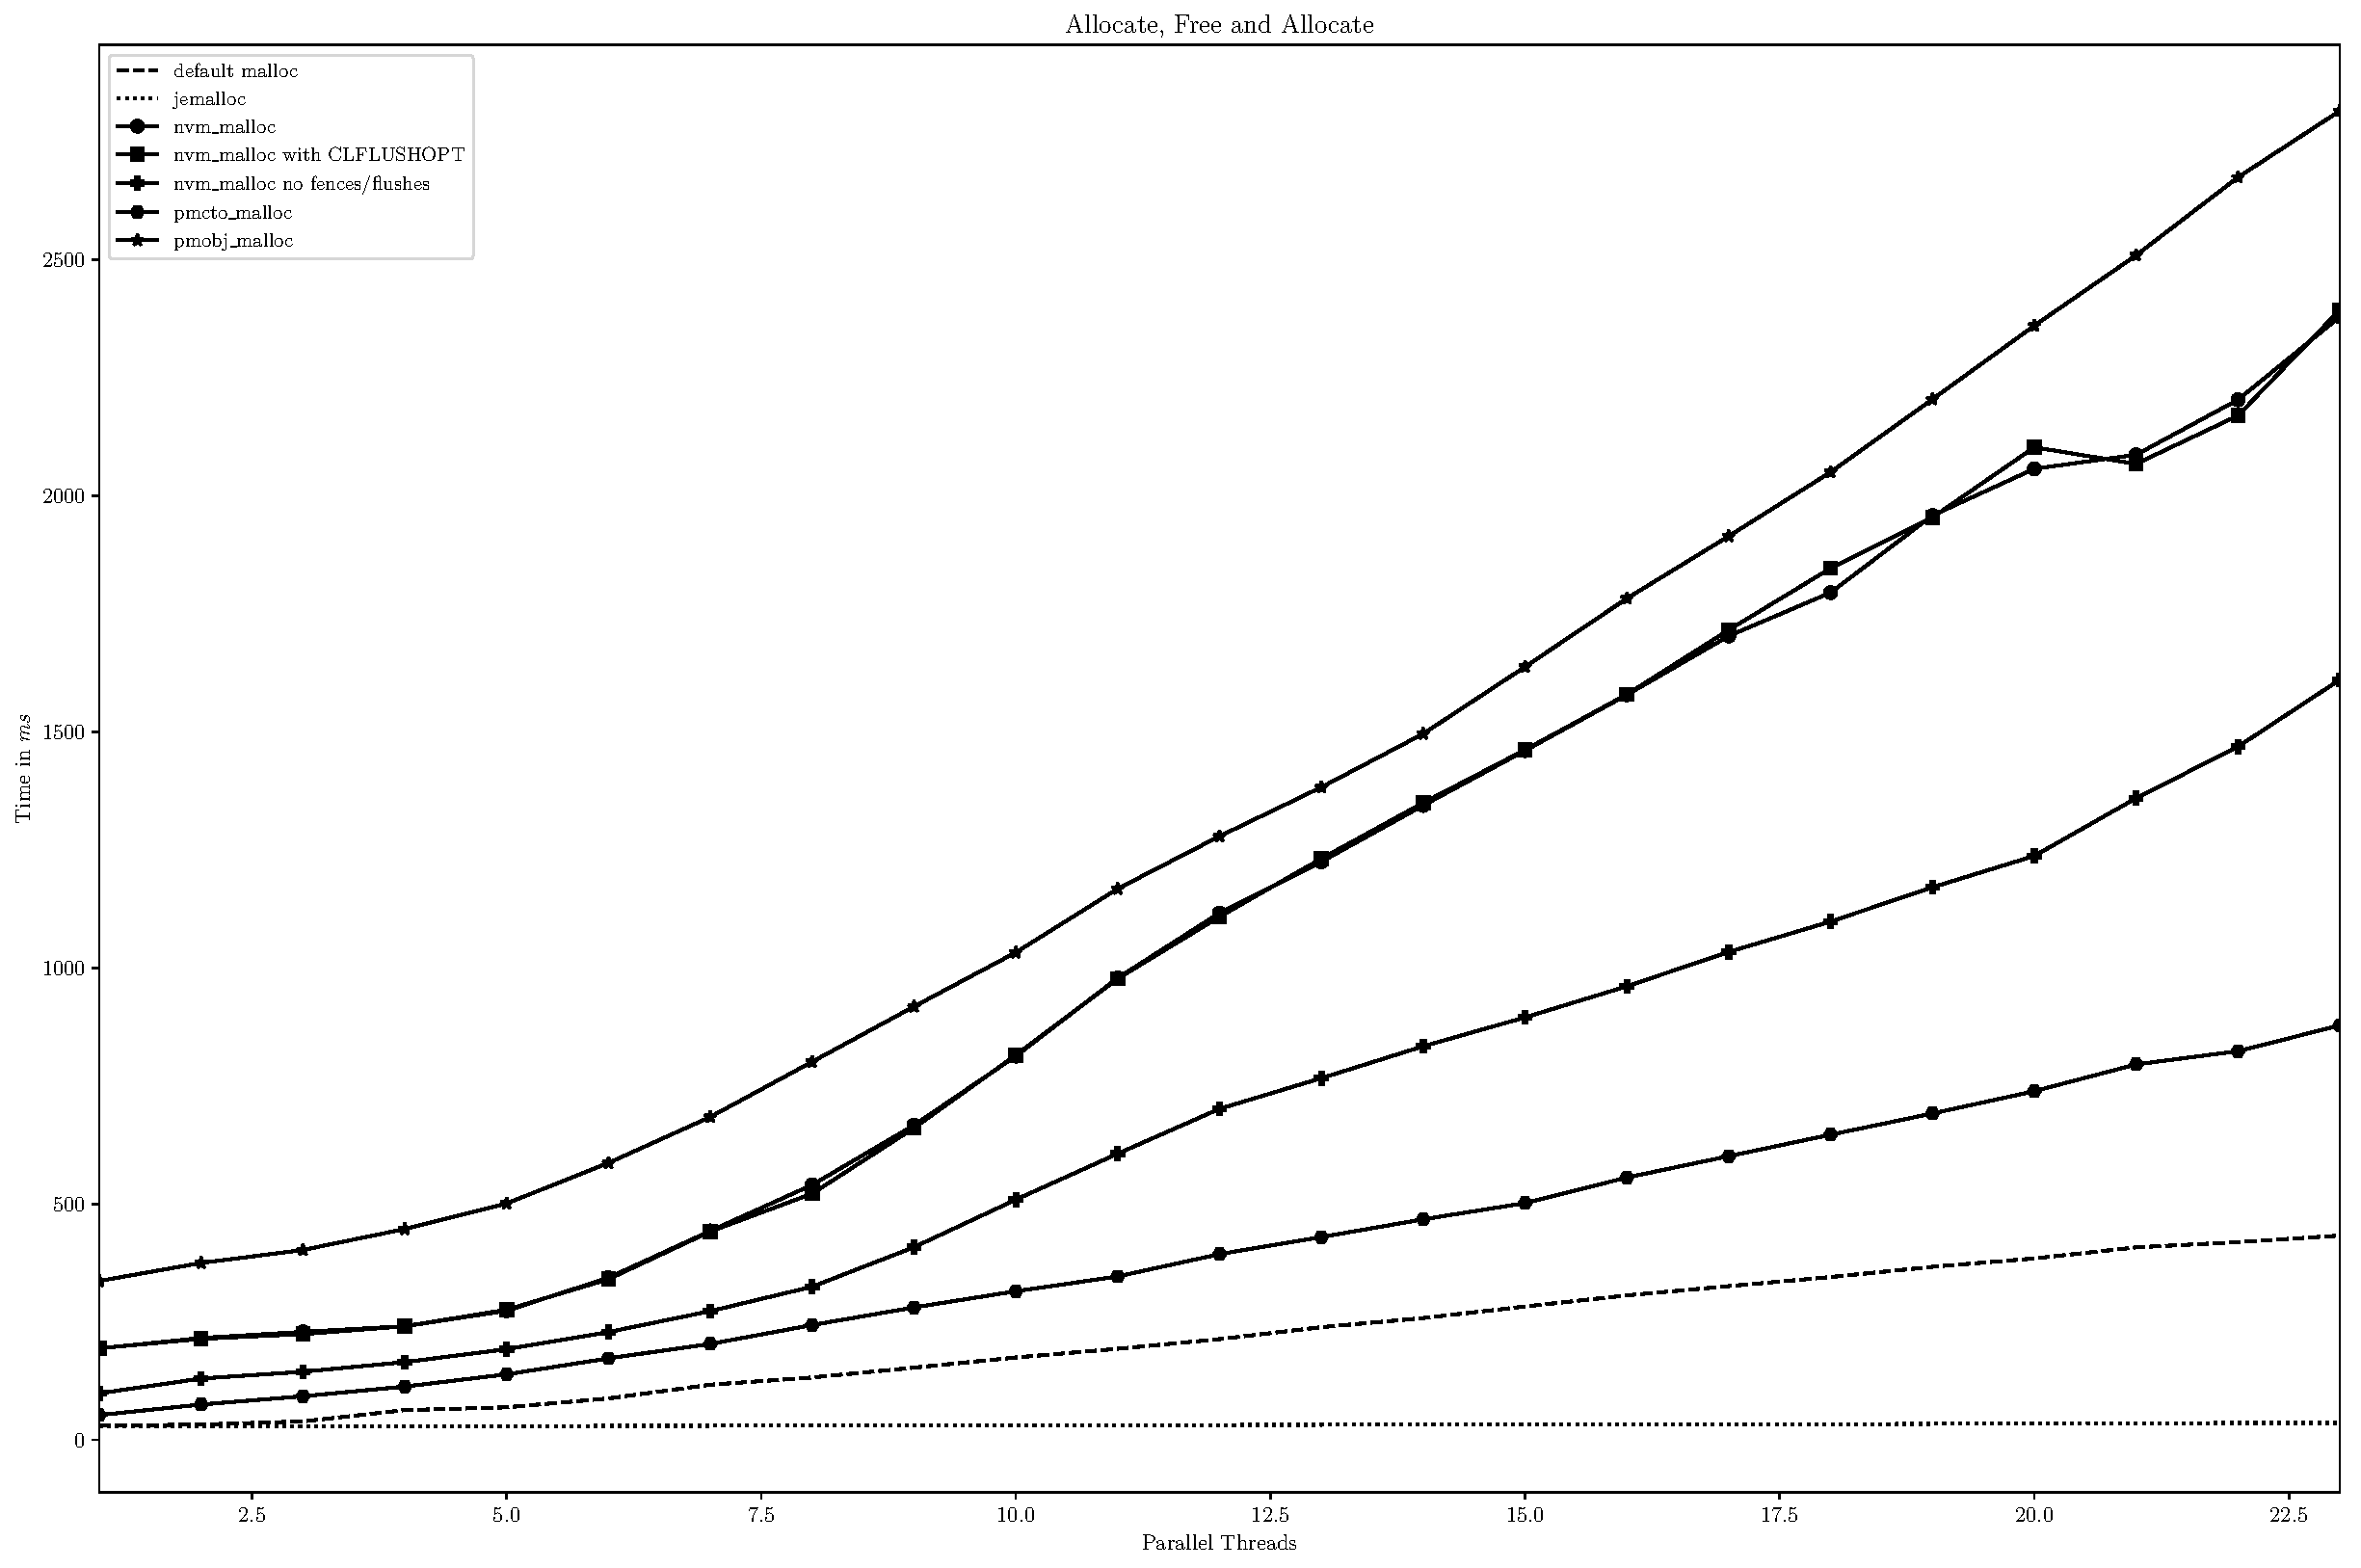
\includegraphics[scale=0.35]{malloc/alloc_free_alloc.pdf}
\end{figure}


\begin{figure}
    \centering
    \caption{Memory Allocation Tests (Alloc-Free)}\label{plot:af}
    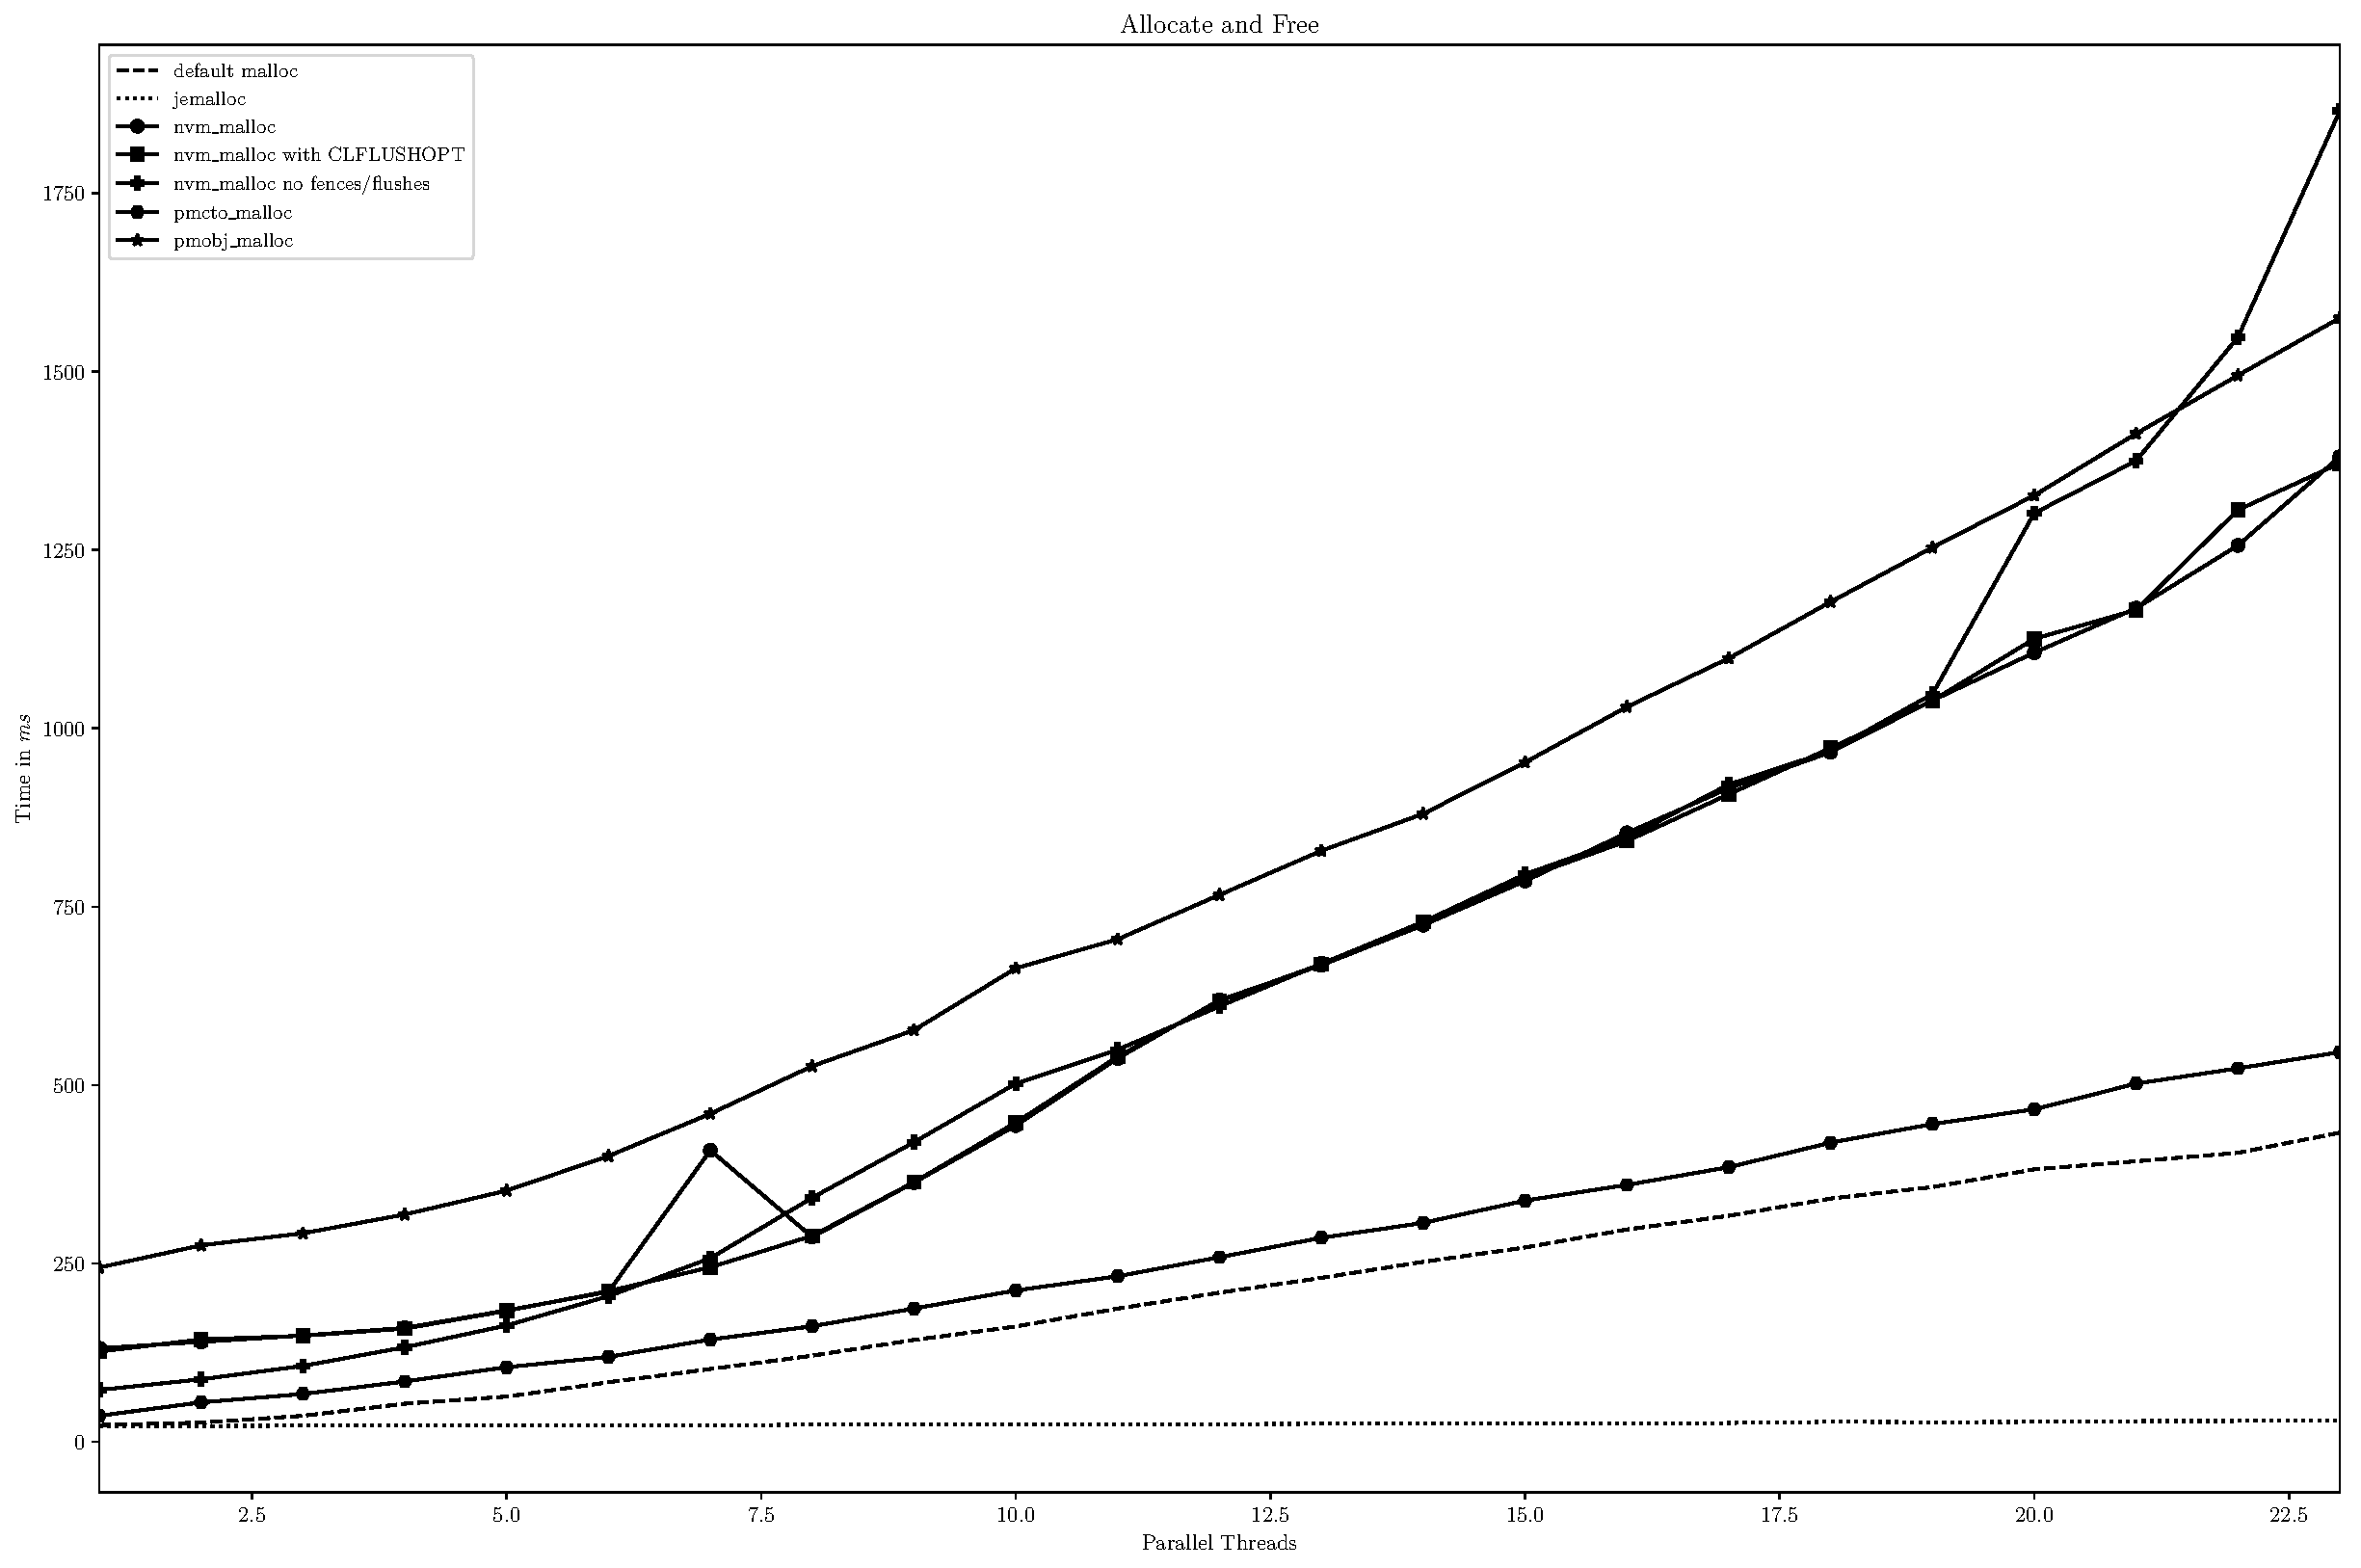
\includegraphics[scale=0.35]{malloc/alloc_free.pdf}
\end{figure}

\begin{figure}
    \centering
    \caption{Memory Allocation Tests (Fastalloc)}\label{plot:fastalloc}
    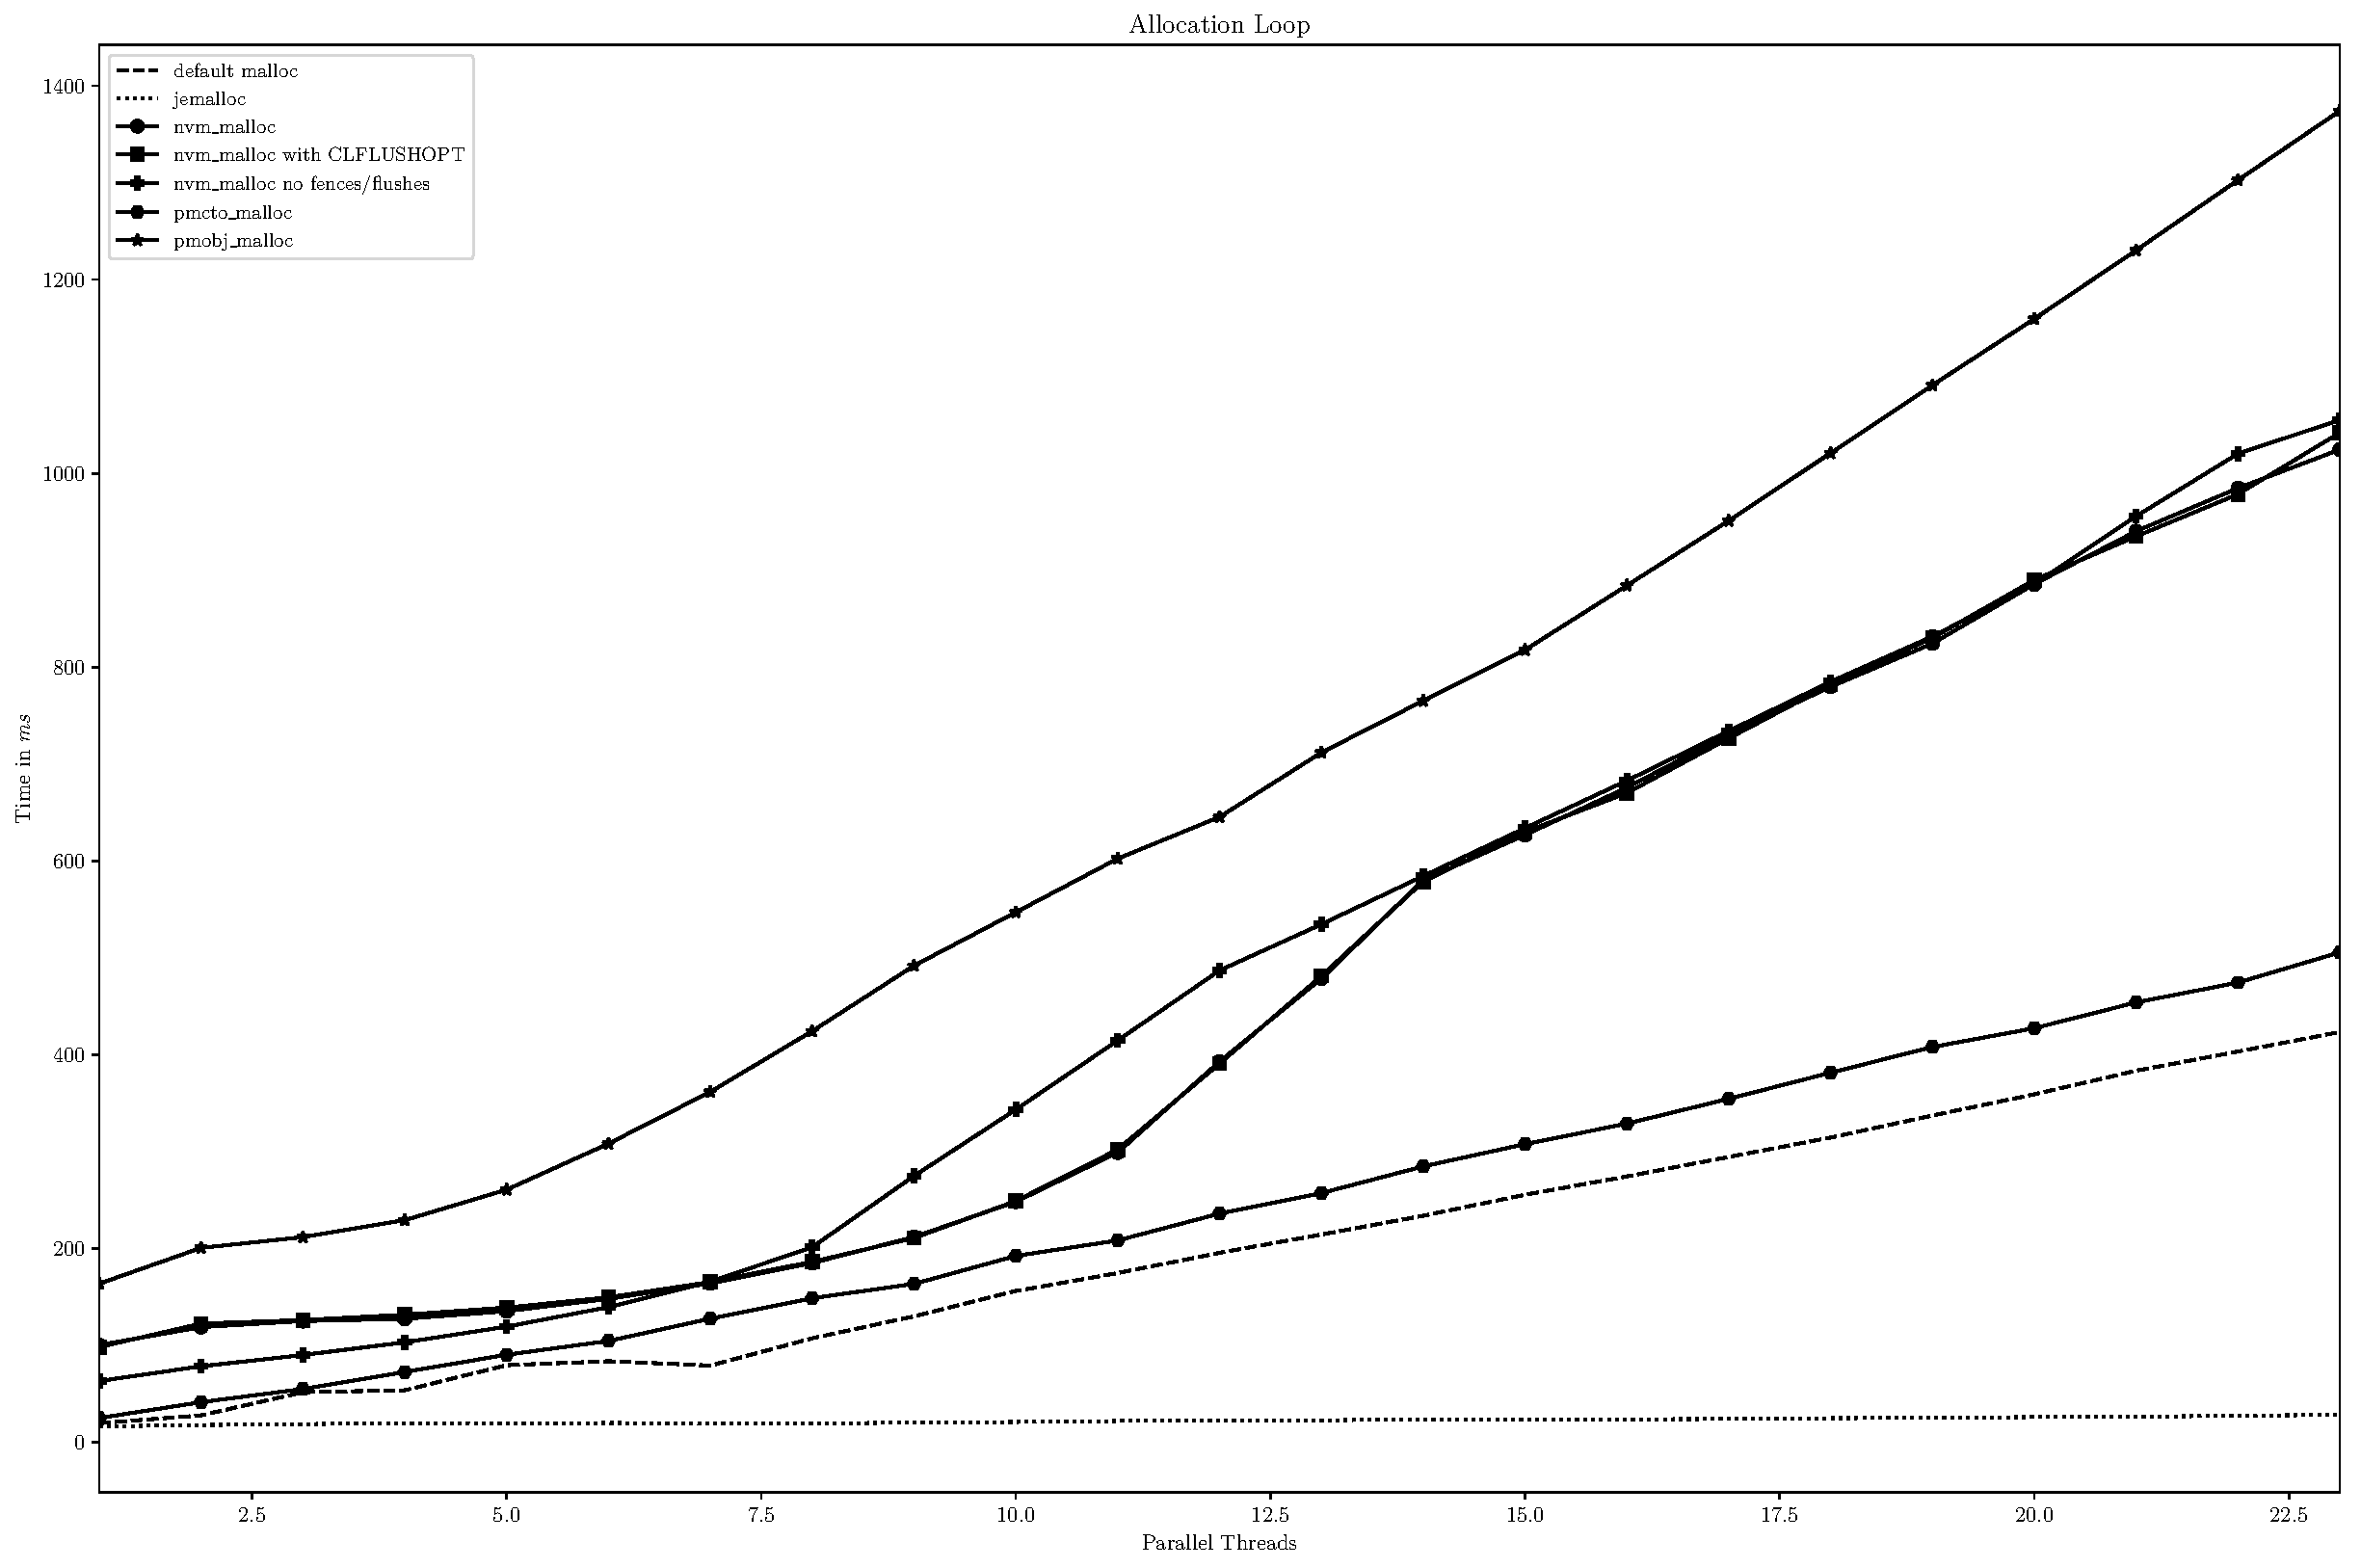
\includegraphics[scale=0.35]{malloc/fastalloc.pdf}
\end{figure}

\begin{figure}
    \centering
    \caption{Memory Allocation Tests (Linkedlist)}\label{plot:linkedlist}
    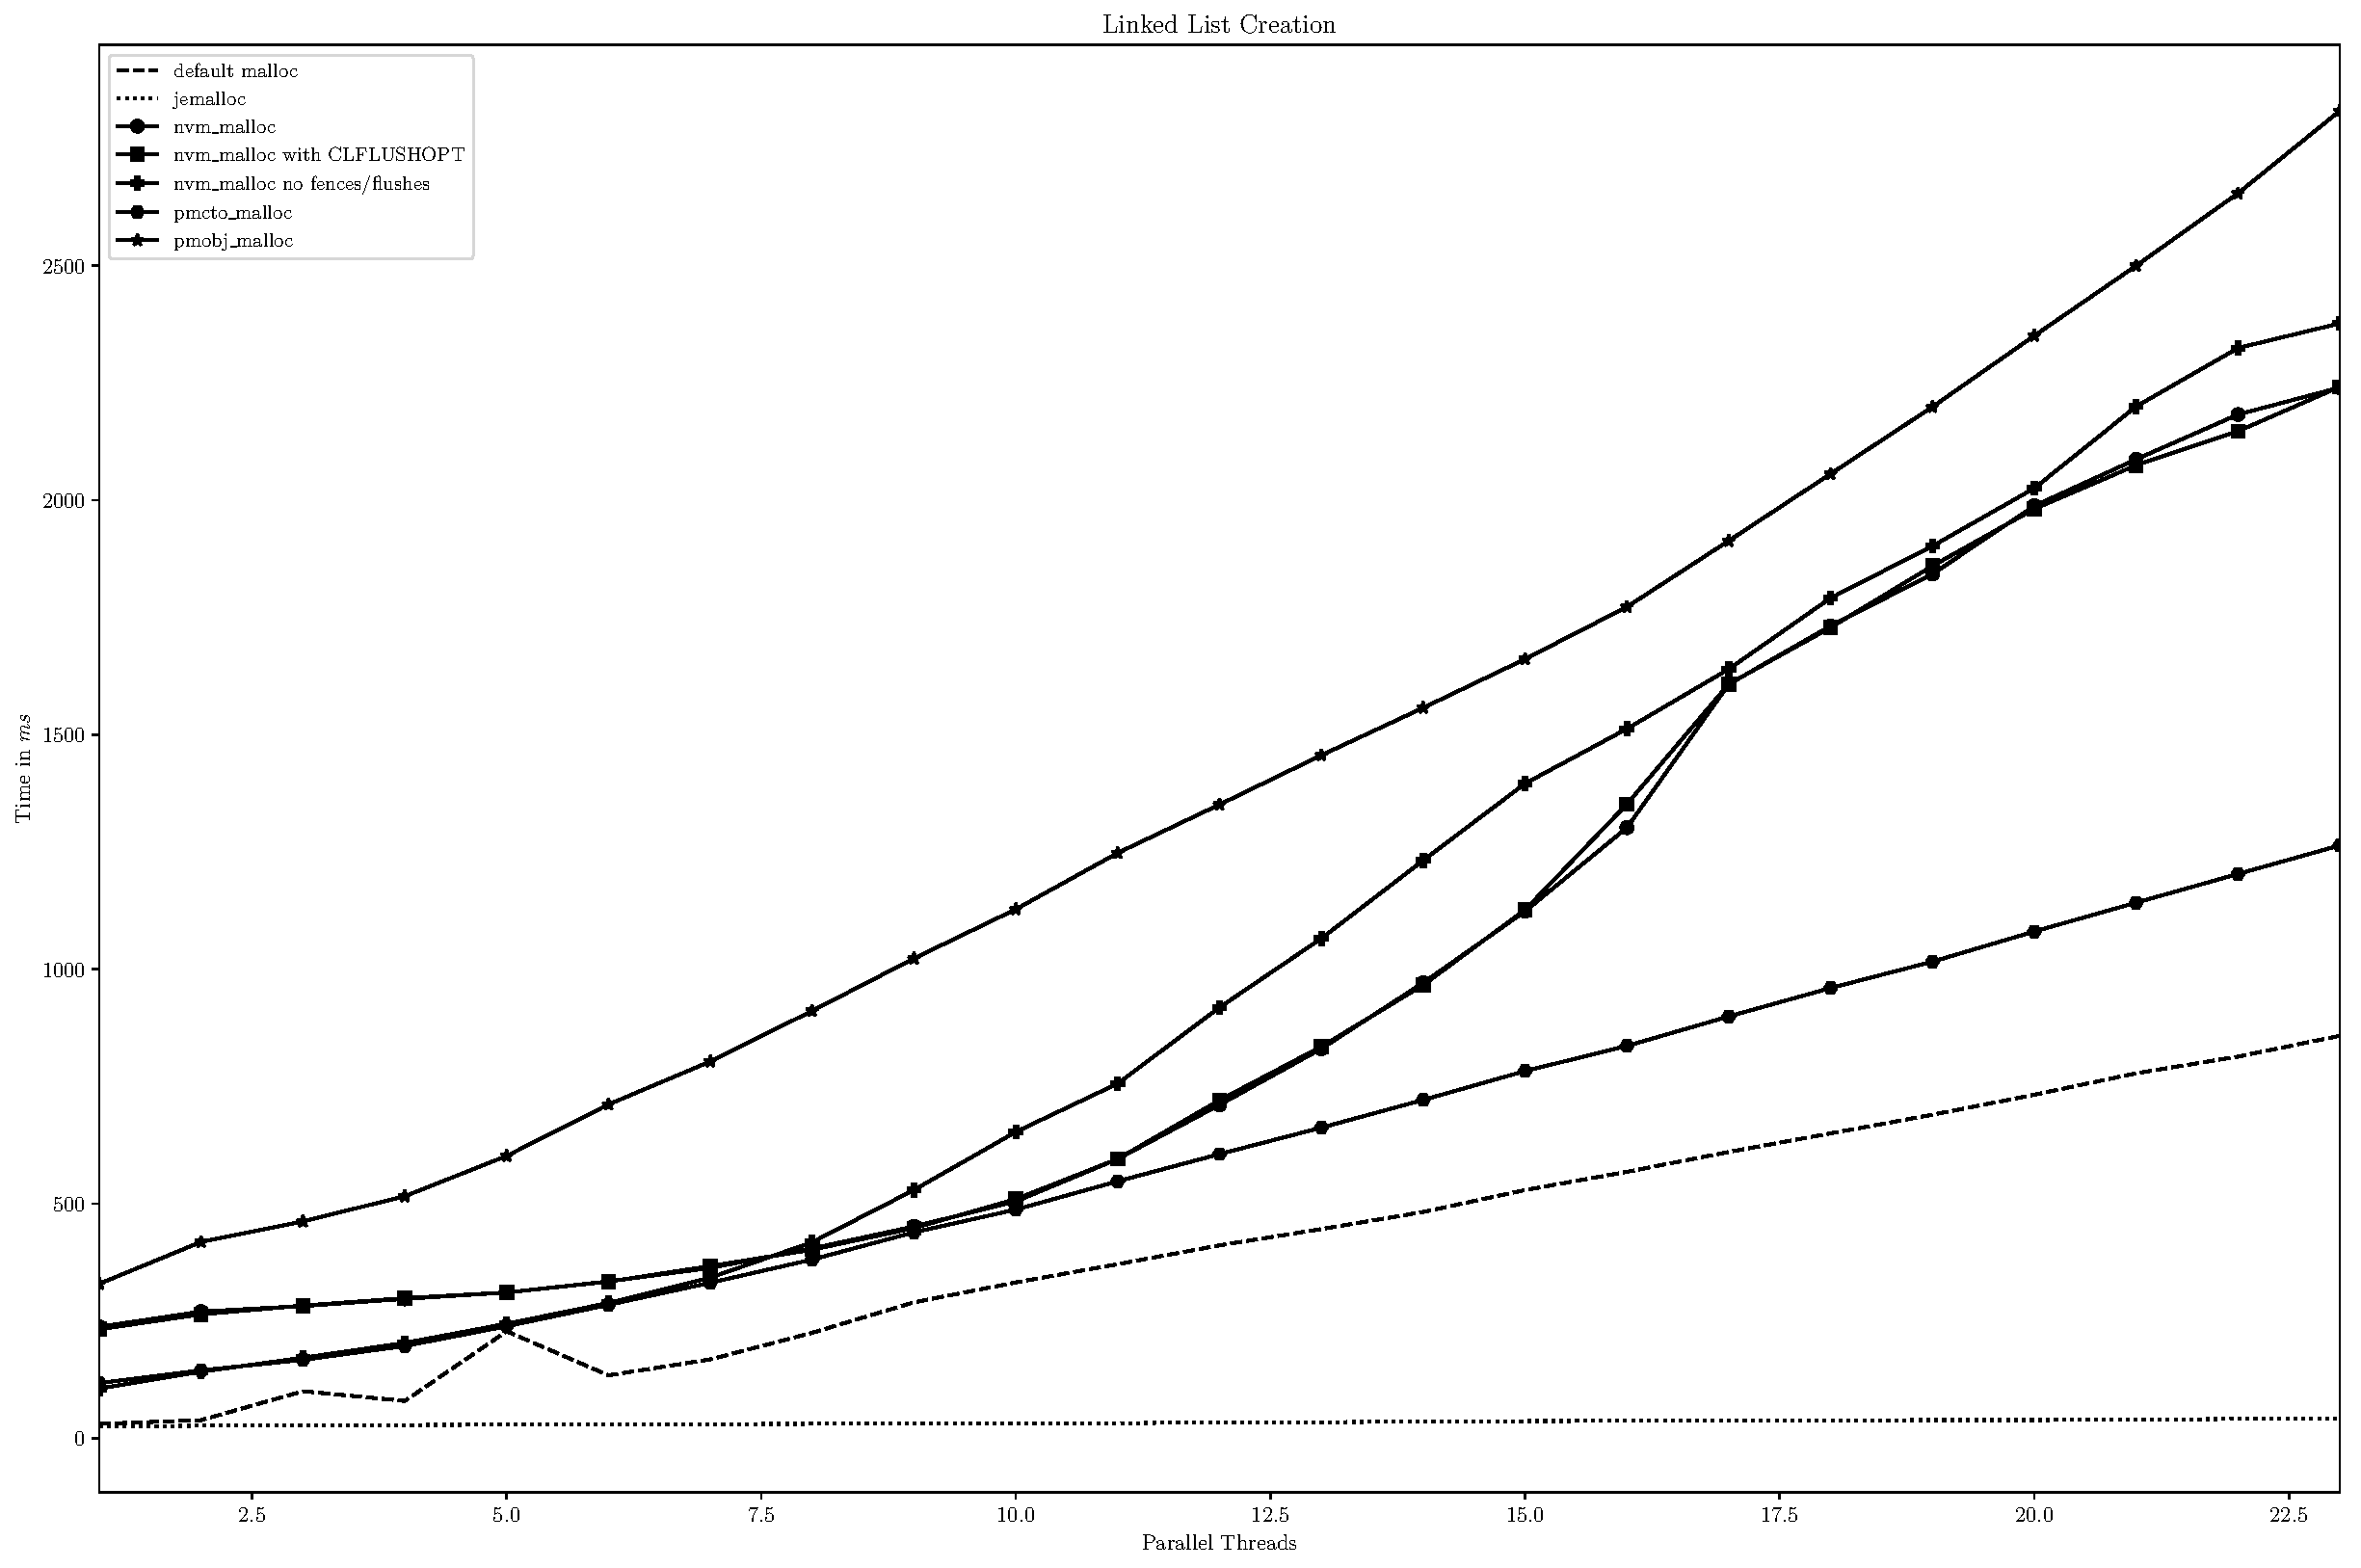
\includegraphics[scale=0.35]{malloc/linkedlist.pdf}
\end{figure}


\endinput



-R read-only load generated, if this is used, -W option should NOT be used 
-Wn where n means
  2  - 2:1 read-write ratio
  3  - 3:1 read-write ratio
  5  - 1:1 read-write ratio
  7  - 2:1 read-Non Temporal Write ratio
  8  - 1:1 read-Non Temporal Write ratio
  10 - 2:1 read-Non Temporal Write ratio (stream triad-like)


dram-baseline-nt-write-same-node.pdf
nt-write-both-nodes.pdf
random-r.pdf
random-W2.pdf
random-W5.pdf
random-w6.pdf
random-W7.pdf
random-W8.pdf
sequential-r.pdf
sequential-w10.pdf
sequential-W2.pdf
sequential-w3.pdf
sequential-W5.pdf
sequential-w6.pdf
sequential-W7.pdf

aep_eval_bandwidth-crop.pdf
aep_eval_idle_latency-crop.pdf
aep_eval_random_read_load_latency-crop.pdf
node-specific-latency-versus-delay-crop.pdf
node-specific-load-data-crop.pdf

